%% The "\appendix" call has already been made in the declaration
%% of the "appendices" environment (see thesis.tex).
\chapter{Search strategy/Appendices}
\label{app:analysis}

%\chapterquote{%
%Le savant n'\'etudie pas la nature parce que cela est utile; \\
%\indent il l'\'etudie parce qu'il y prend plaisir, \\
%\indent et il y prend plaisir parce qu'elle est belle.}%
%{Henri Poincar\'e, 1854--1912}

%Appendixes (or should that be ``appendices''?) make you look really clever, 
%%%'cos it's like you had more clever stuff to say than could be fitted into 
%%%the %%%%main bit of your thesis. Yeah. So everyone should have at least 
%%%%%%%three of %%%%%them\dots

%% Big appendixes should be split off into separate files, just like chapters
%\input{app-myreallybigappendix}

%Data/MC plots or 
plots showing the contributions of different backgrounds in 
the SR/CRs. And/or yields (section 4 in AN).

\section{Uncertainties on transfer factors derived from variations in 
simulation}
\label{app:tfvariations}
This appendix shows the changes of the transfer factors, which are used to 
assign systematic uncertainties to them, upon varying the various correction 
factors applied to the simulation (Sec.~\ref{sec:analysis-mccorrections}) by 
one standard deviation up and down according to their measured uncertainties.

\begin{figure}[h!]
	\subfloat{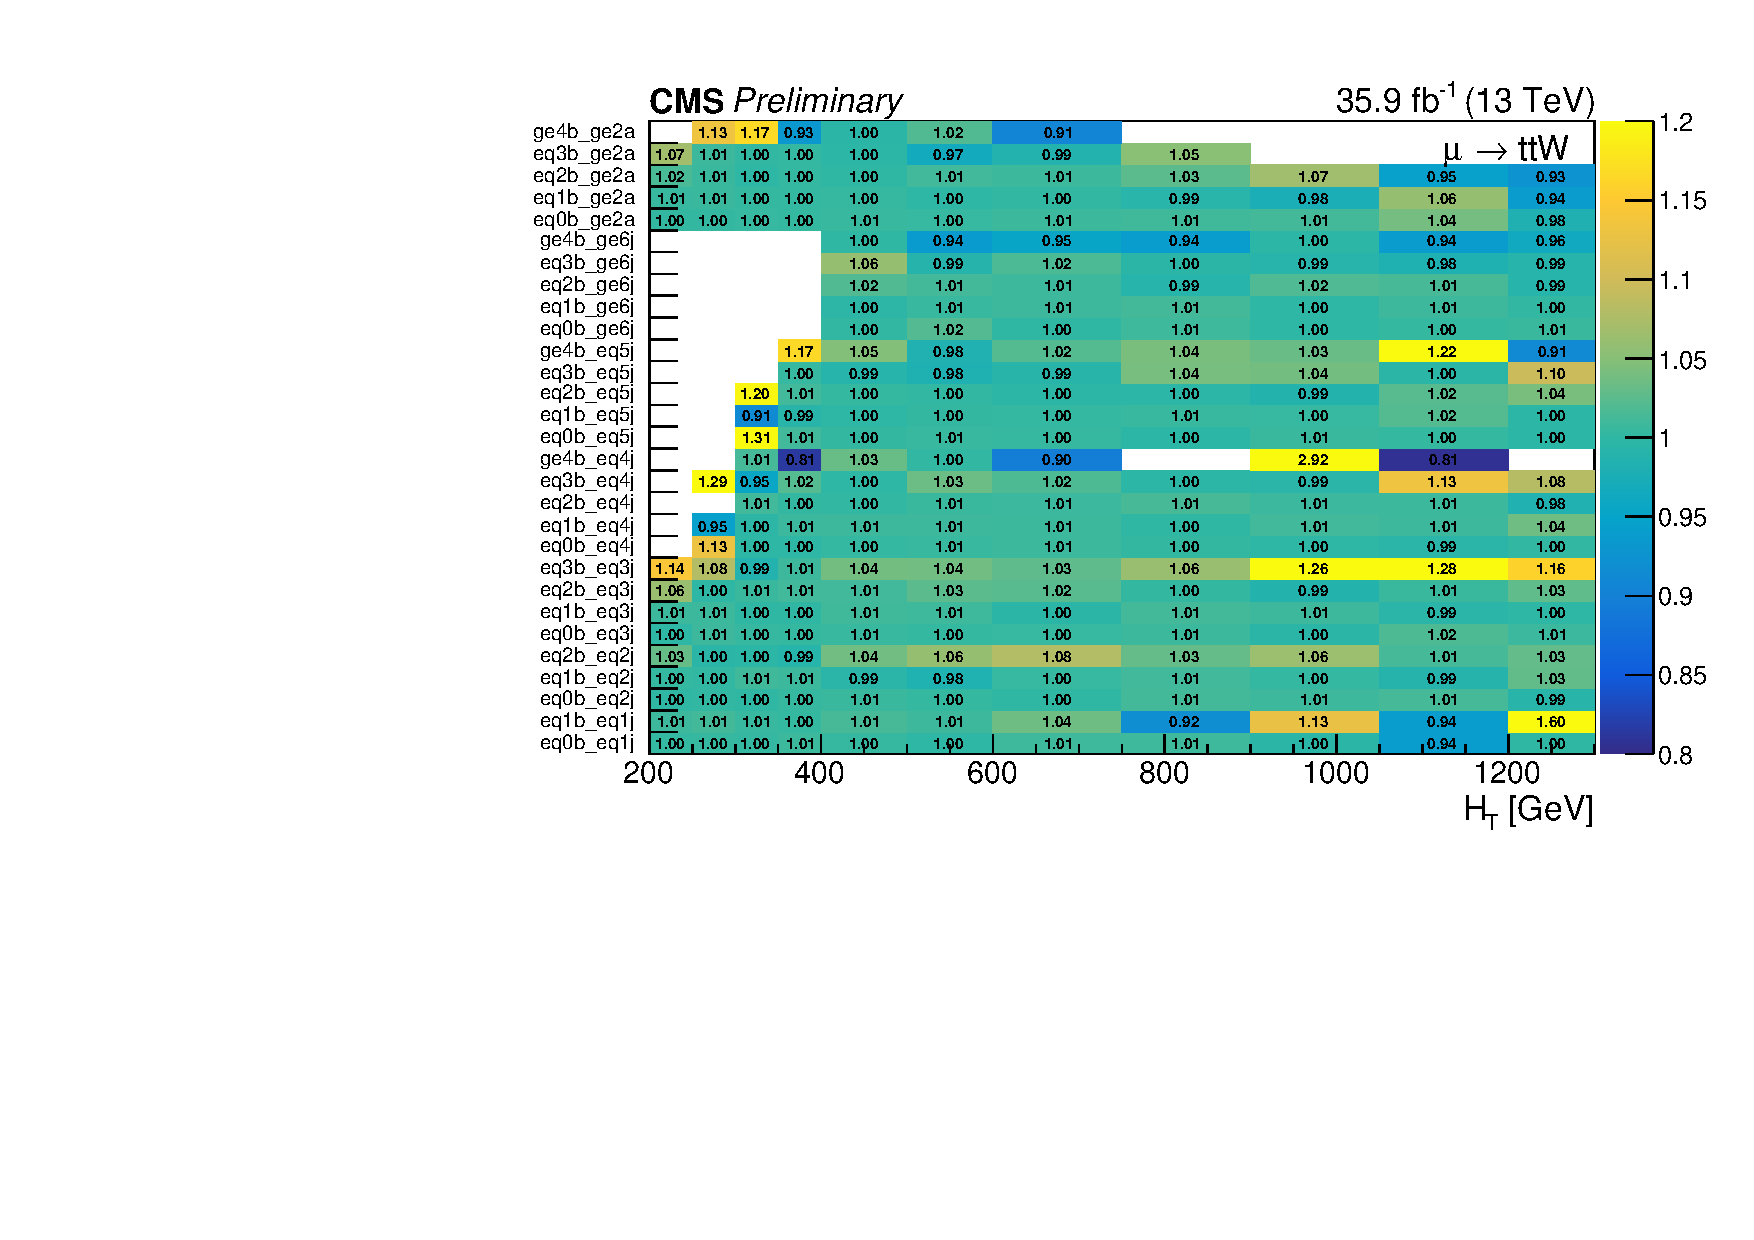
\includegraphics[width=0.5\textwidth]{figs/analysis/transferfactors/tfratio_mu_Ttw_2d_puWeightUp}}~
	\subfloat{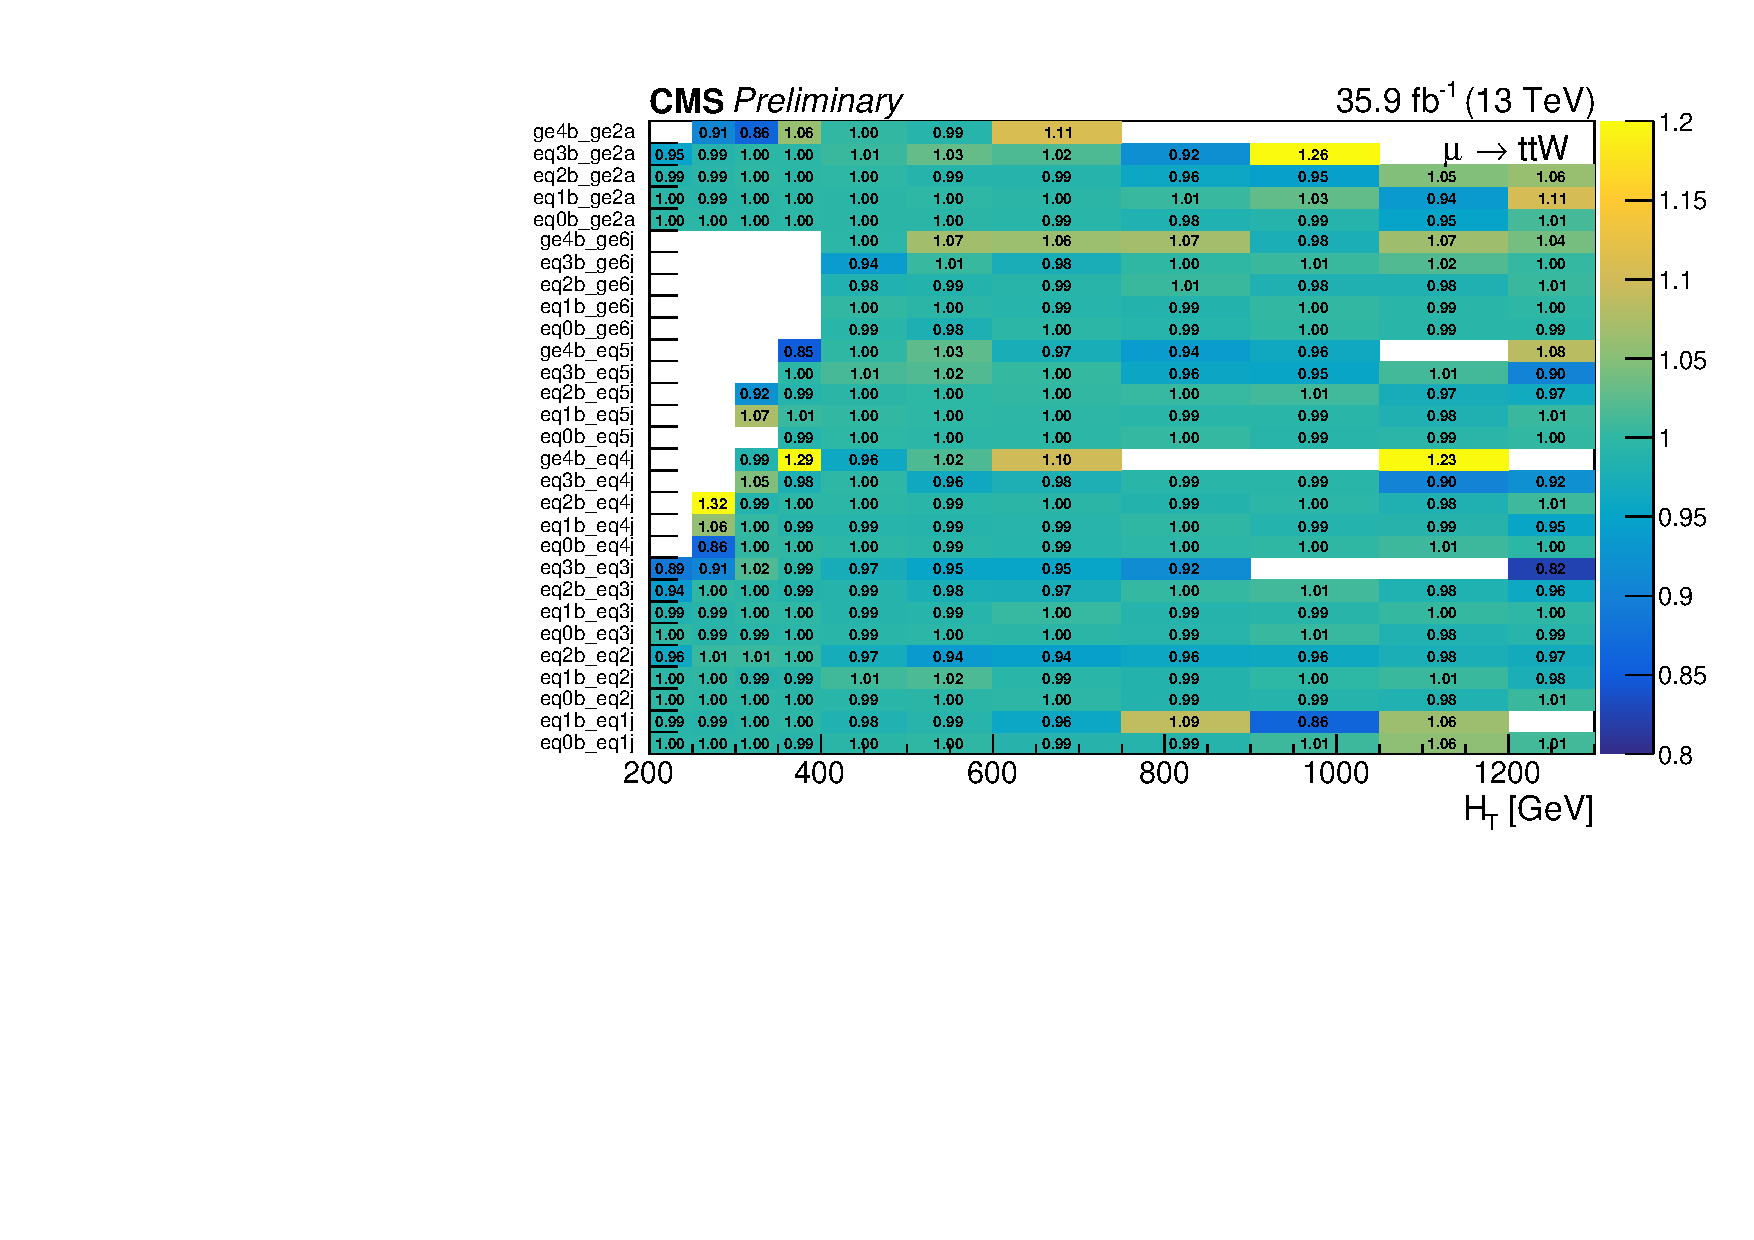
\includegraphics[width=0.5\textwidth]{figs/analysis/transferfactors/tfratio_mu_Ttw_2d_puWeightDown}}\\
	\subfloat{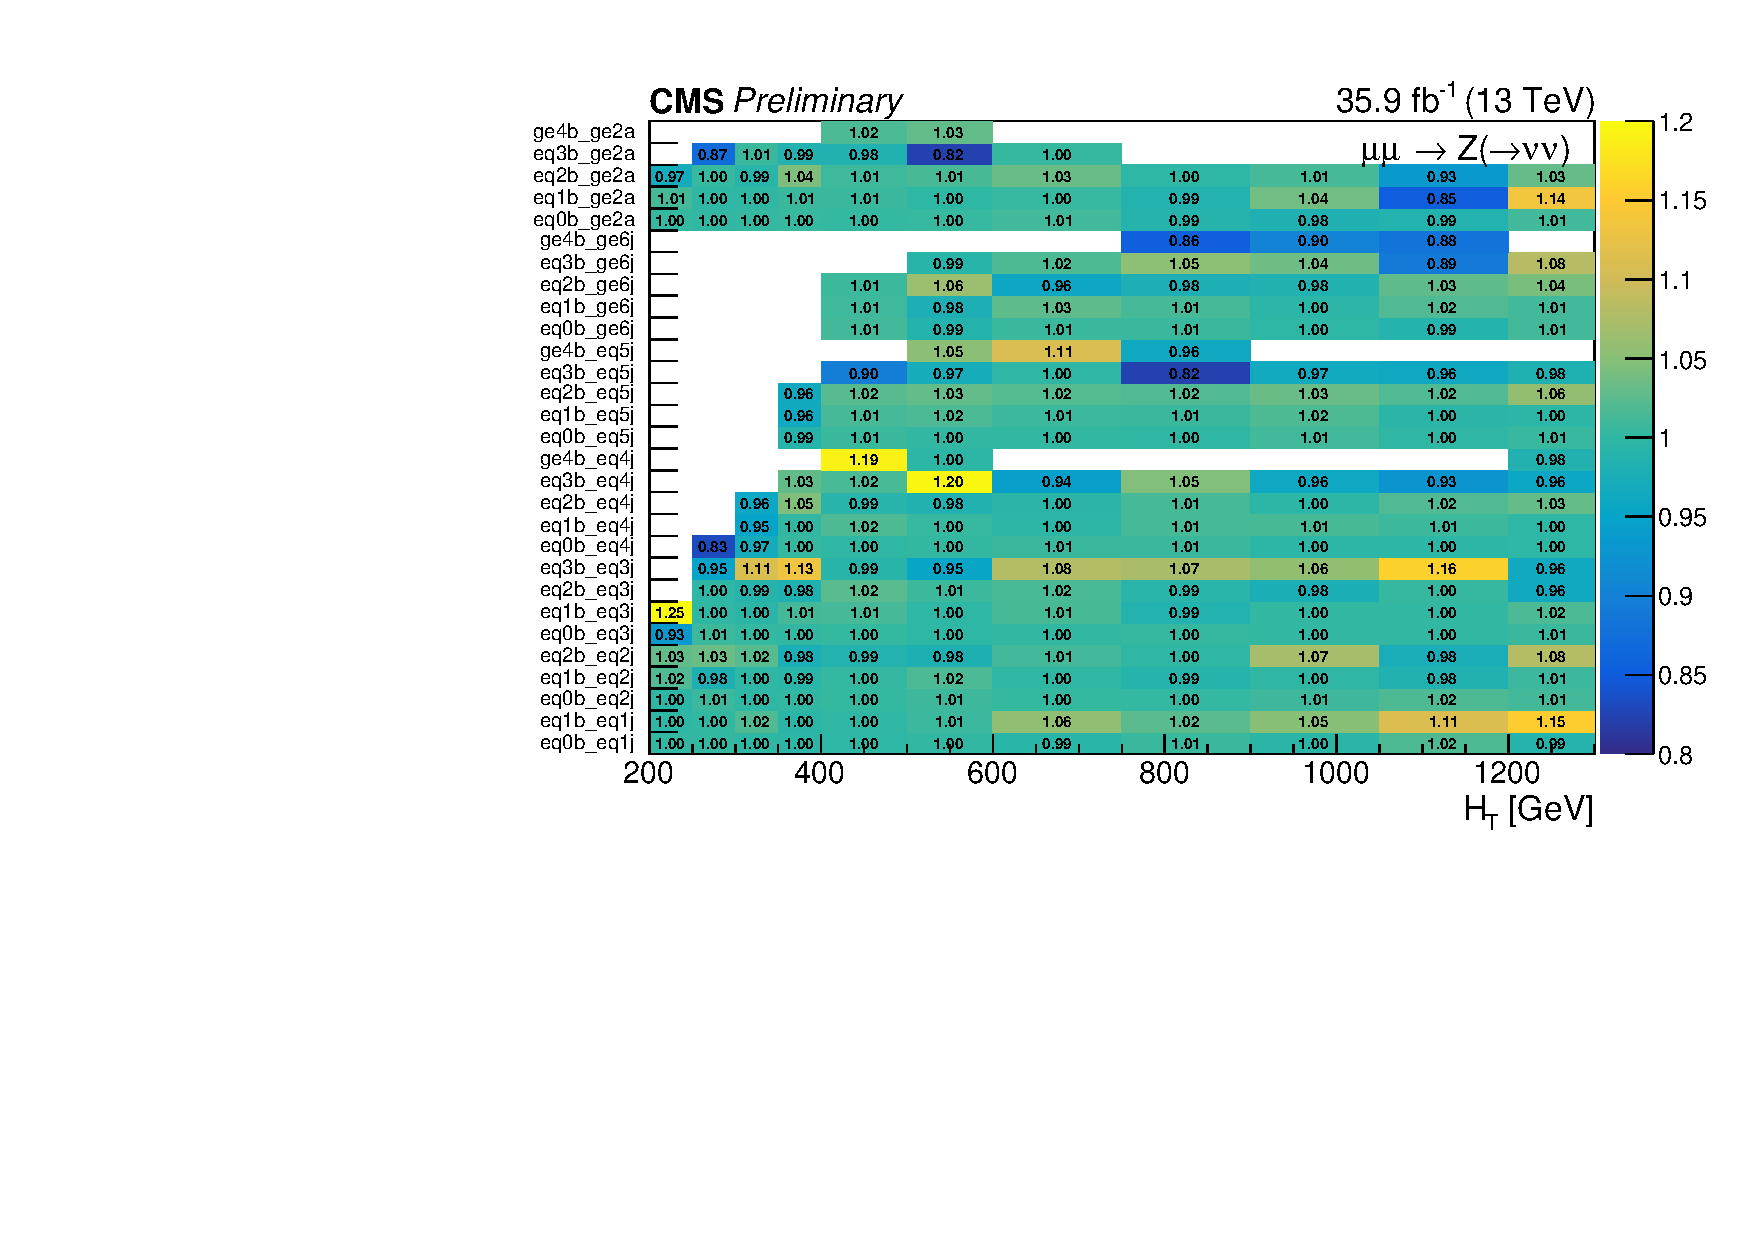
\includegraphics[width=0.5\textwidth]{figs/analysis/transferfactors/tfratio_mumu_Zinv_2d_puWeightUp}}~
	\subfloat{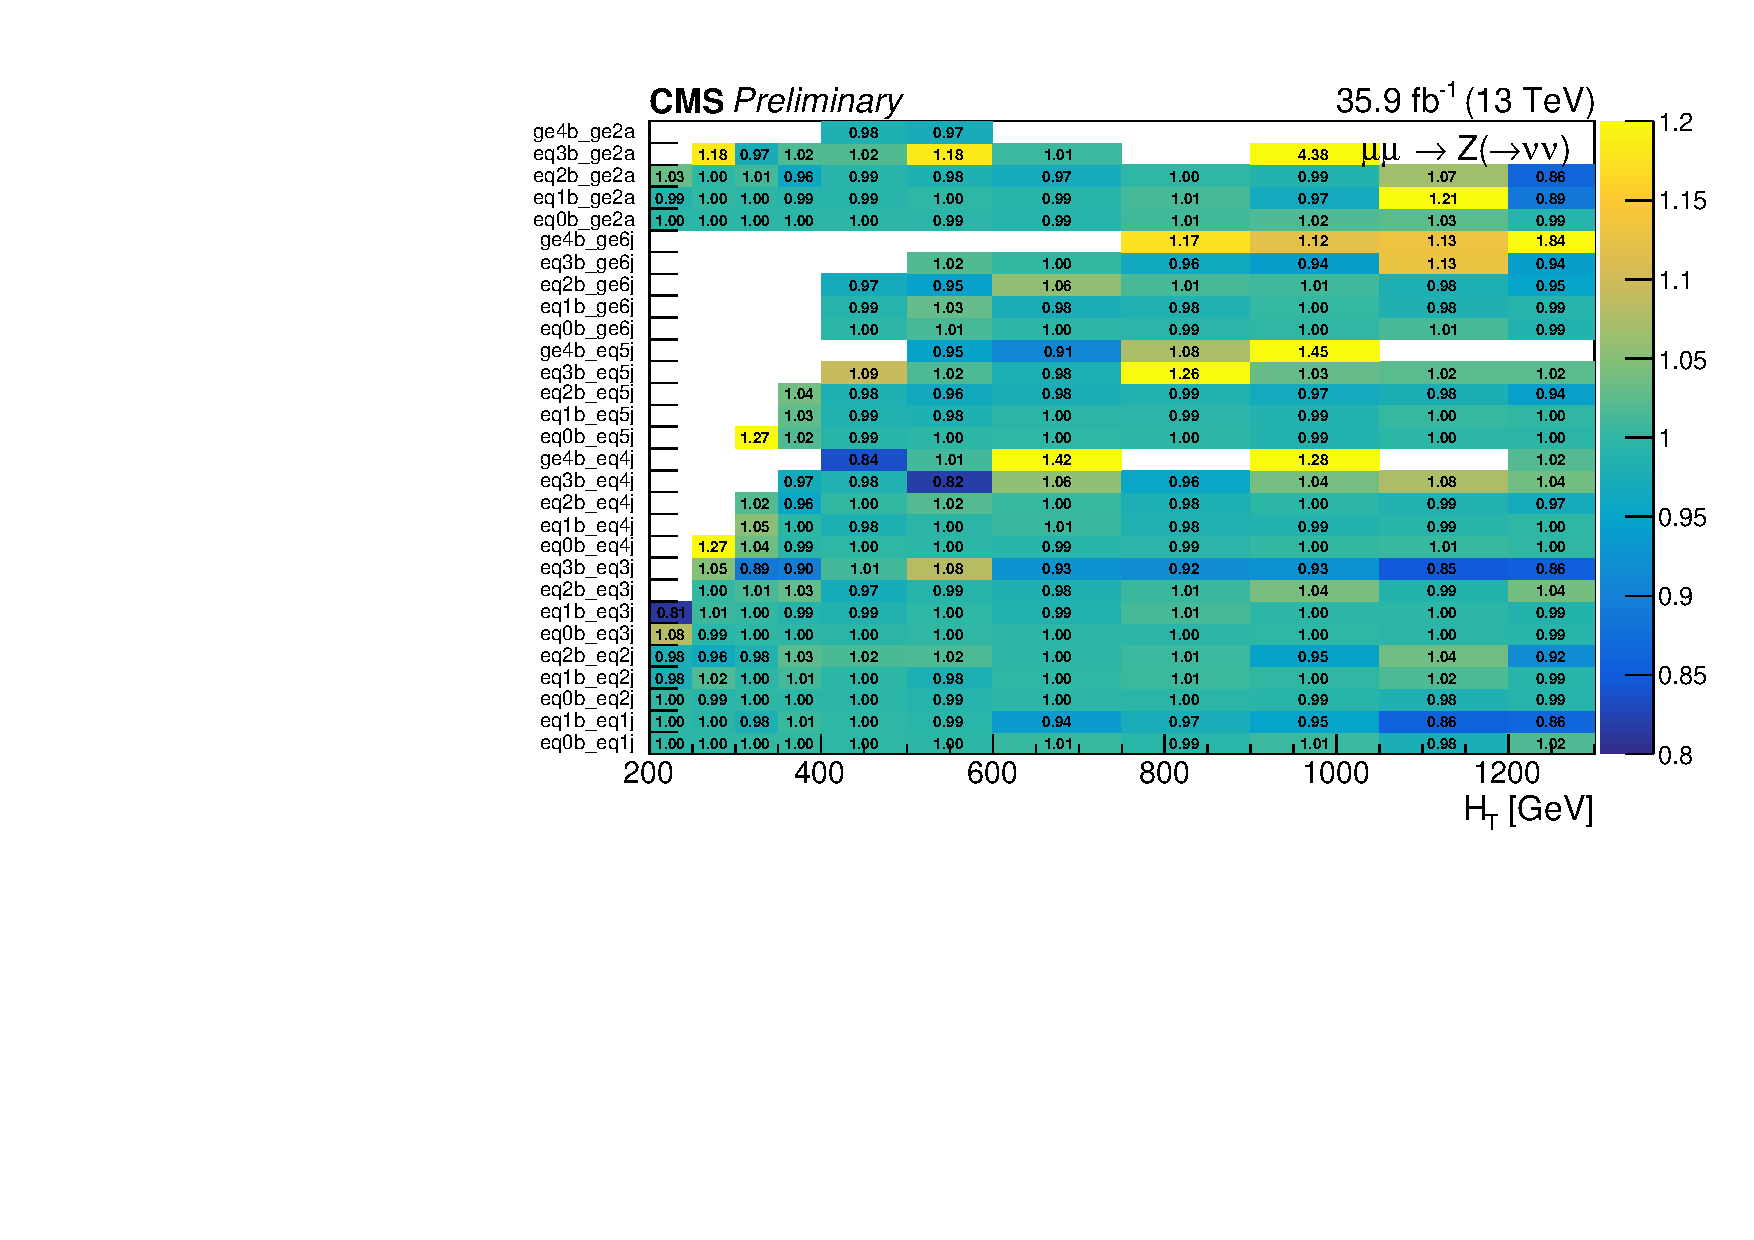
\includegraphics[width=0.5\textwidth]{figs/analysis/transferfactors/tfratio_mumu_Zinv_2d_puWeightDown}}\\
	\caption{The ratio of the \Tmutottw (top) and \Tmumutoz (bottom) transfer 
		factors in each \njnbht bin when varying the pileup correction factors 
		by $+1\sigma$ (left) and $-1\sigma$ (right) with respect to 
		their nominal values.}
	\label{fig:tfvariations-pileup}
\end{figure}

\begin{figure}[h!]
	\subfloat{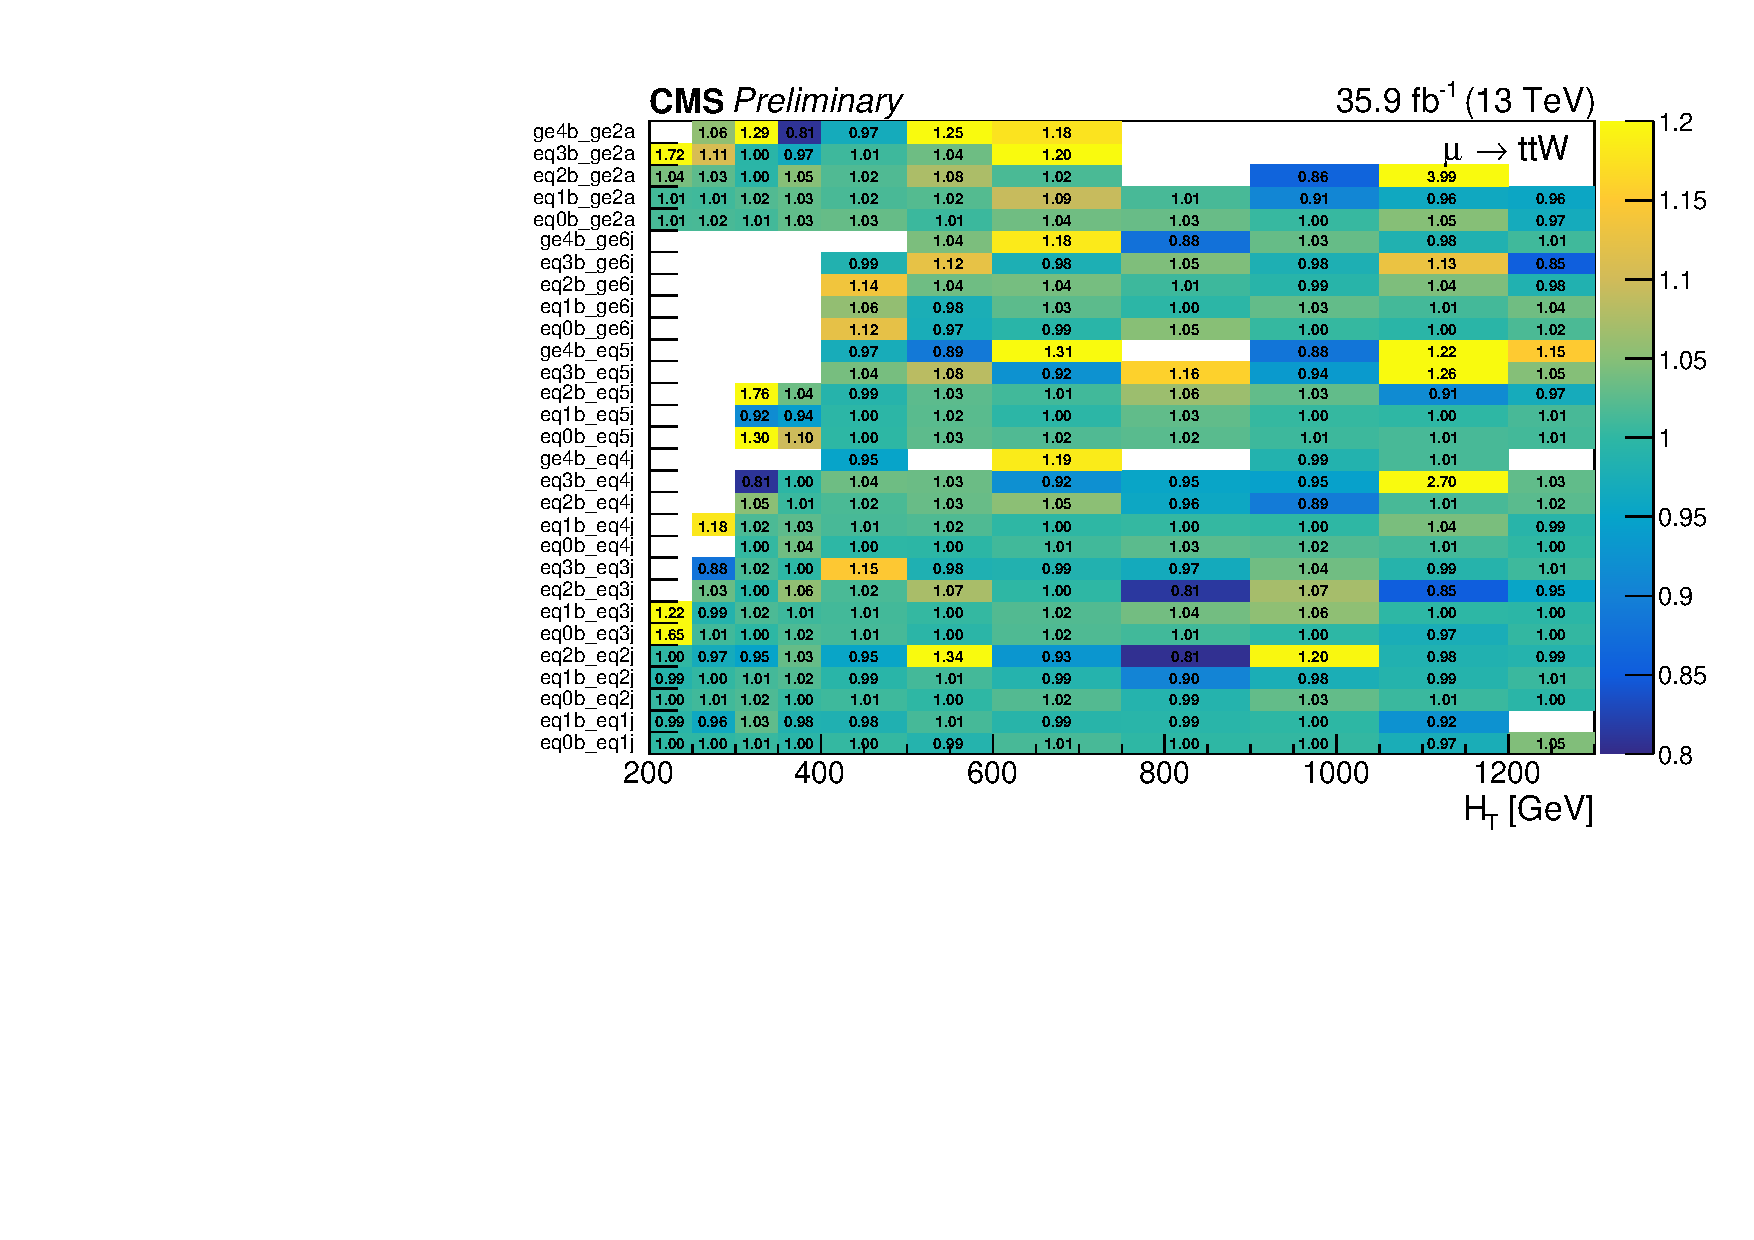
\includegraphics[width=0.5\textwidth]{figs/analysis/transferfactors/tfratio_mu_Ttw_2d_jecUp}}~
	\subfloat{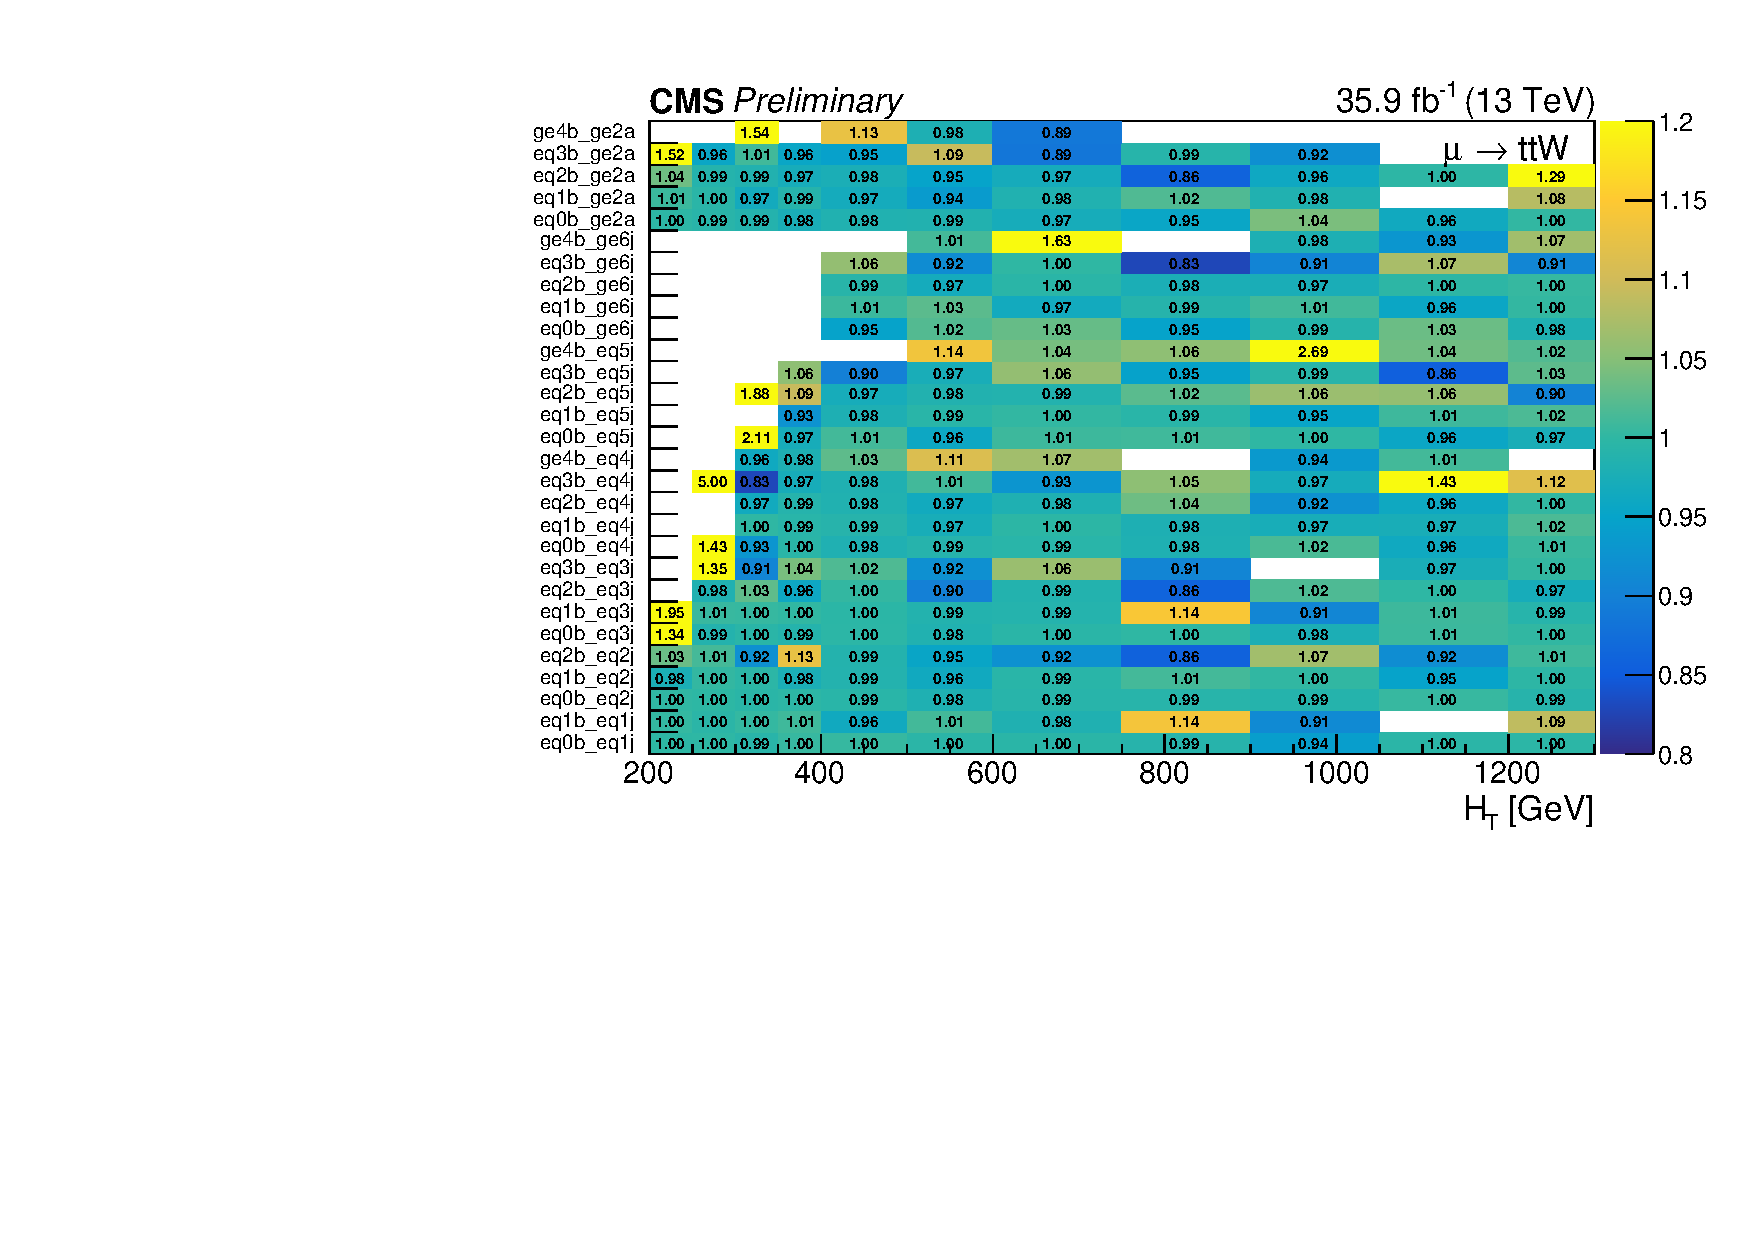
\includegraphics[width=0.5\textwidth]{figs/analysis/transferfactors/tfratio_mu_Ttw_2d_jecDown}}\\
	\subfloat{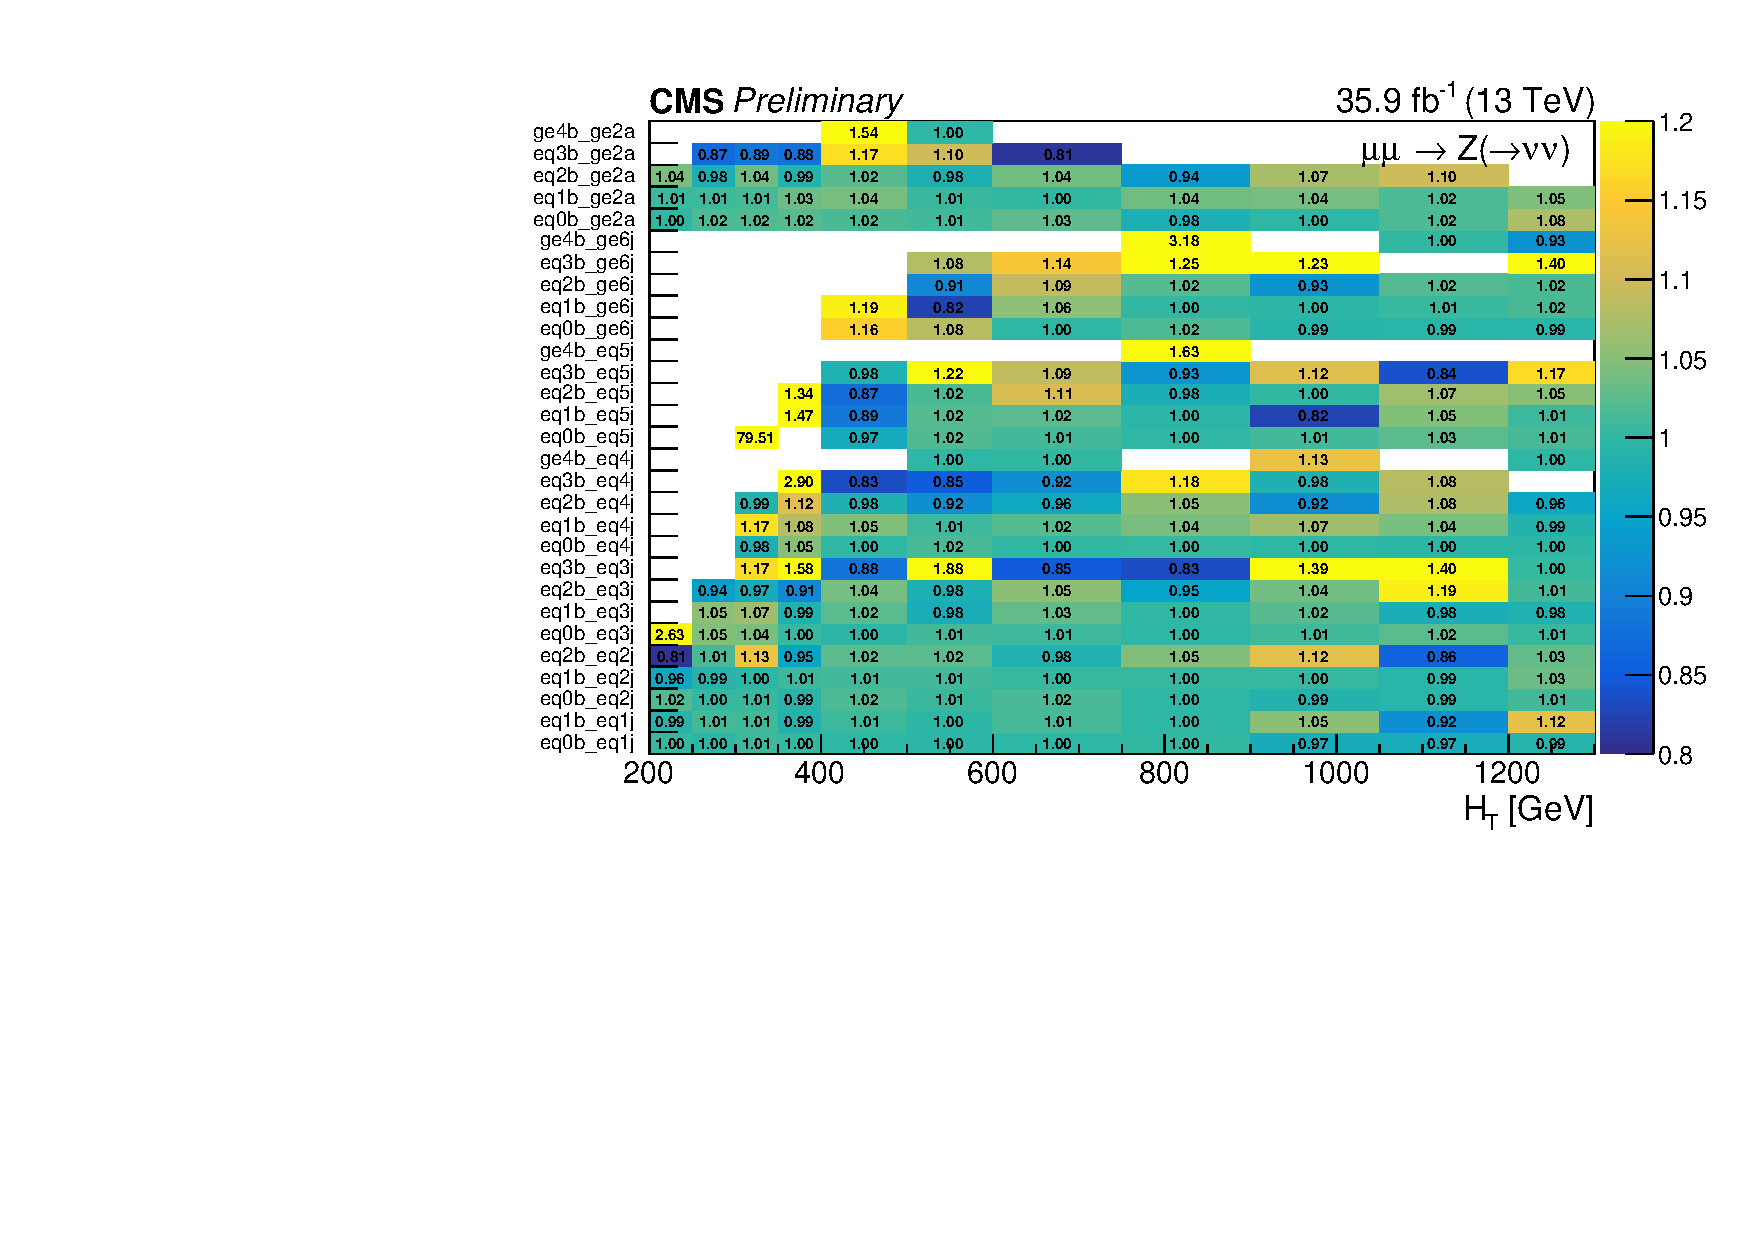
\includegraphics[width=0.5\textwidth]{figs/analysis/transferfactors/tfratio_mumu_Zinv_2d_jecUp}}~
	\subfloat{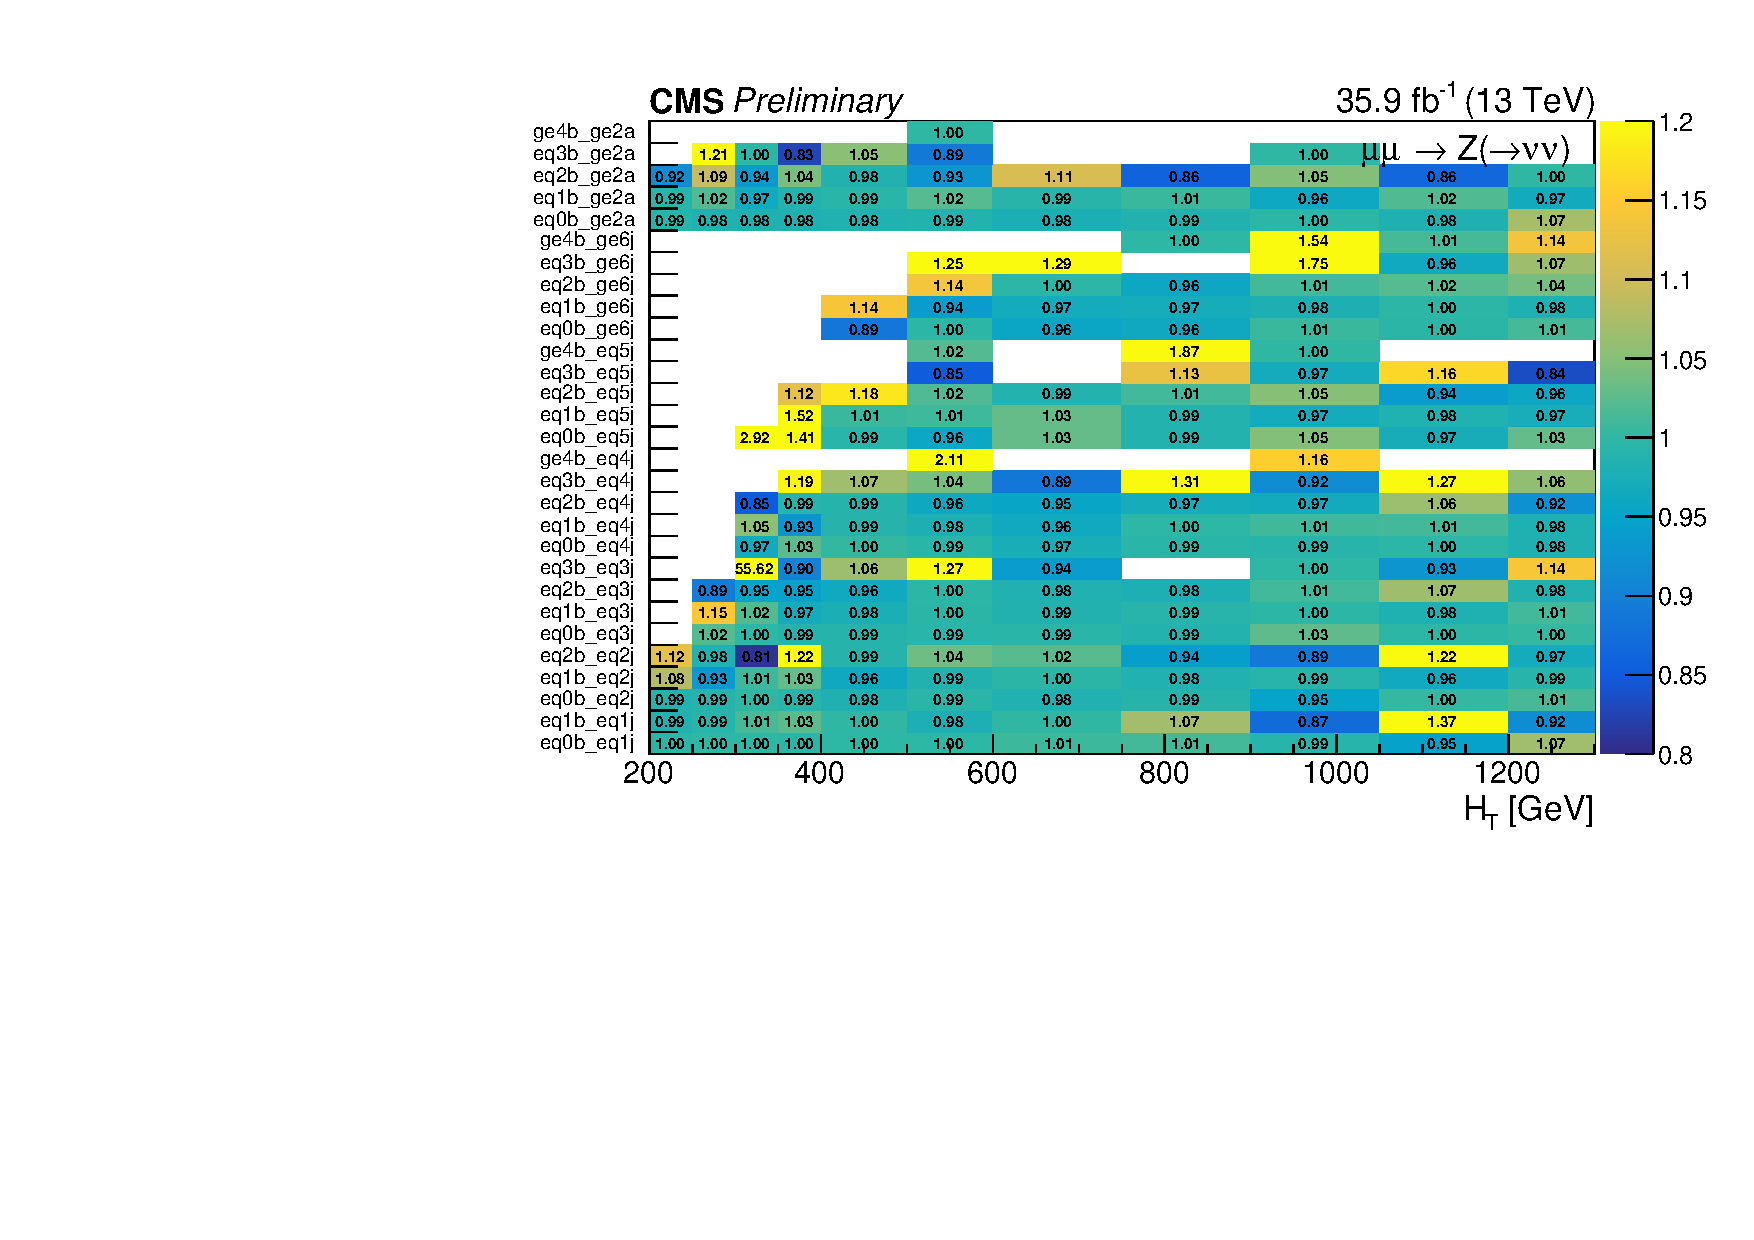
\includegraphics[width=0.5\textwidth]{figs/analysis/transferfactors/tfratio_mumu_Zinv_2d_jecDown}}\\
	\caption{The ratio of the \Tmutottw (top) and \Tmumutoz (bottom) transfer 
		factors in each \njnbht bin when varying the jet energy correction 
		factors by $+1\sigma$ (left) and $-1\sigma$ (right) with respect to 
		their nominal values.}
	\label{fig:tfvariations-jec}
\end{figure}

\begin{figure}[h!]
	\subfloat{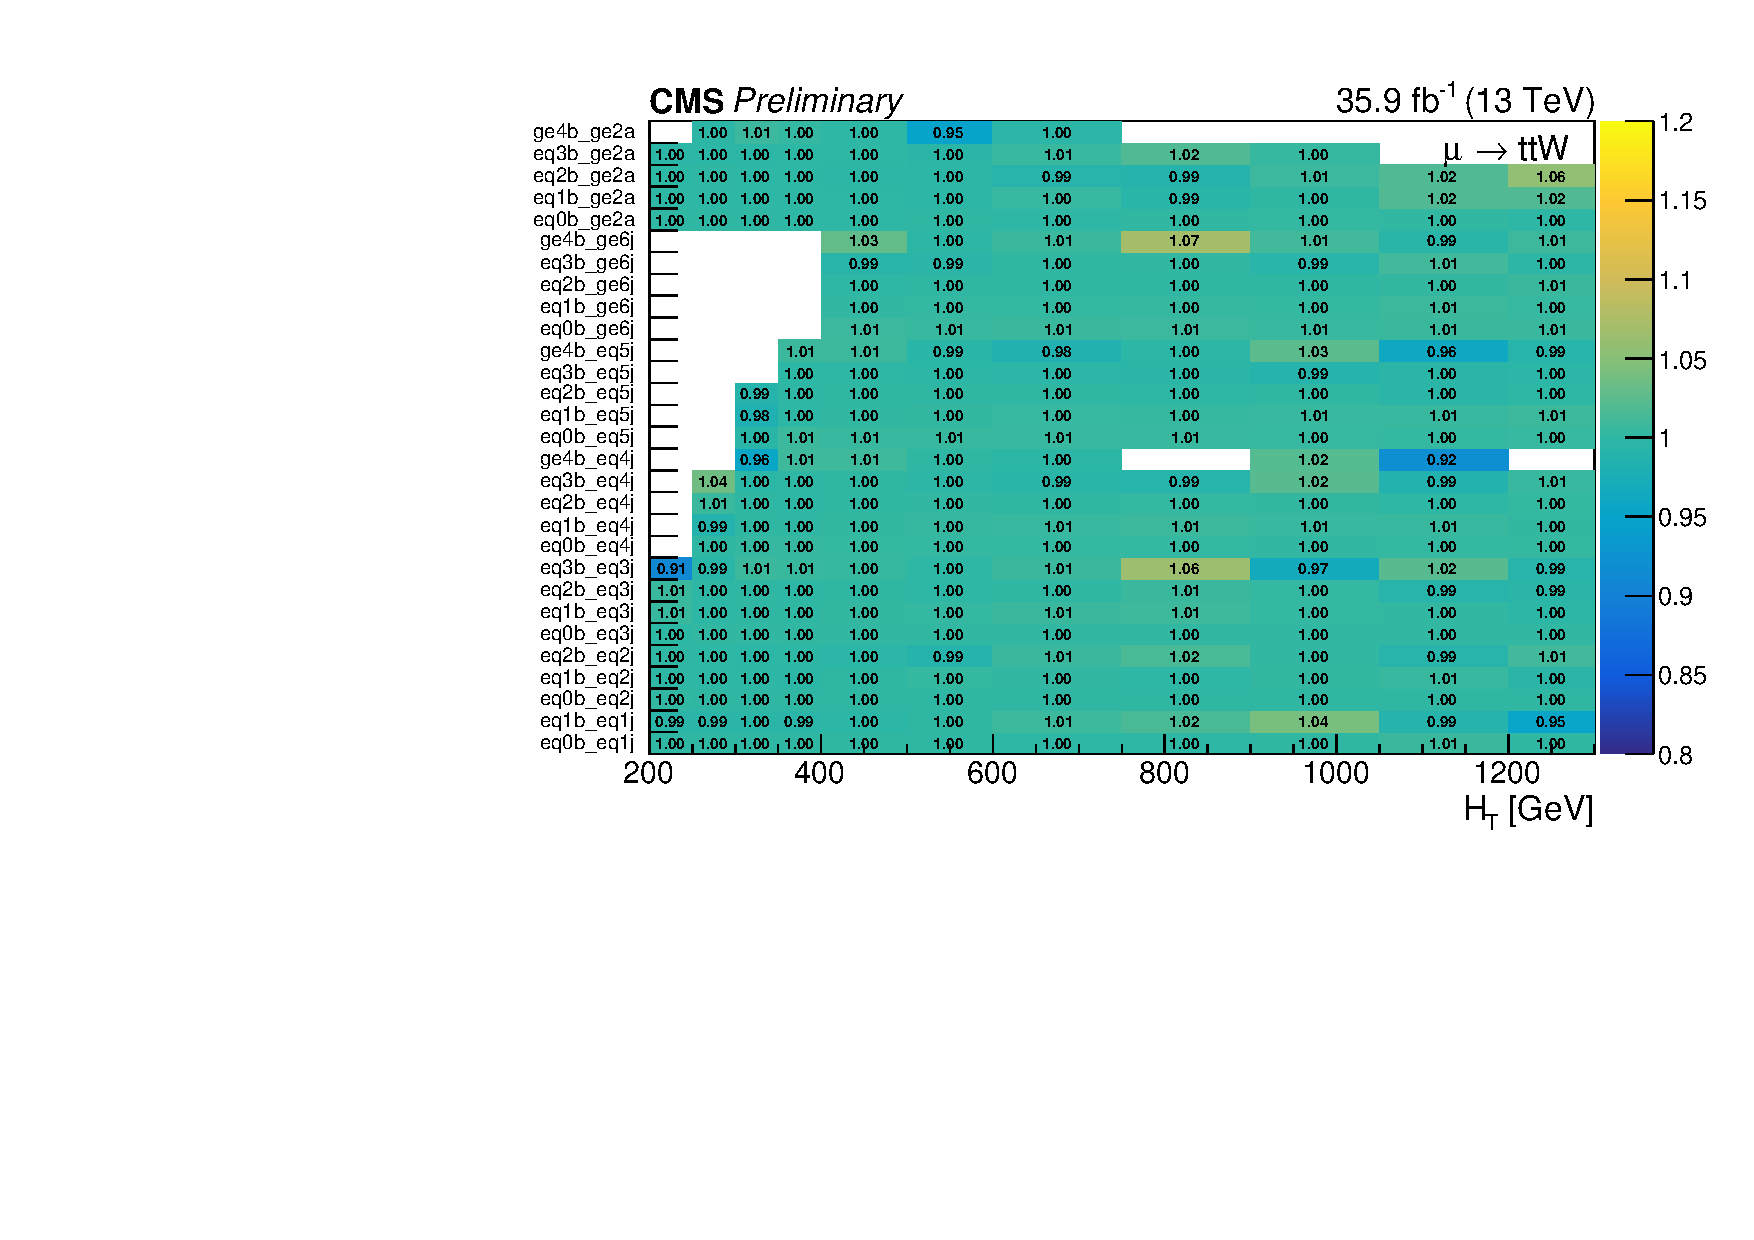
\includegraphics[width=0.5\textwidth]{figs/analysis/transferfactors/tfratio_mu_Ttw_2d_bsfWeightUp}}~
	\subfloat{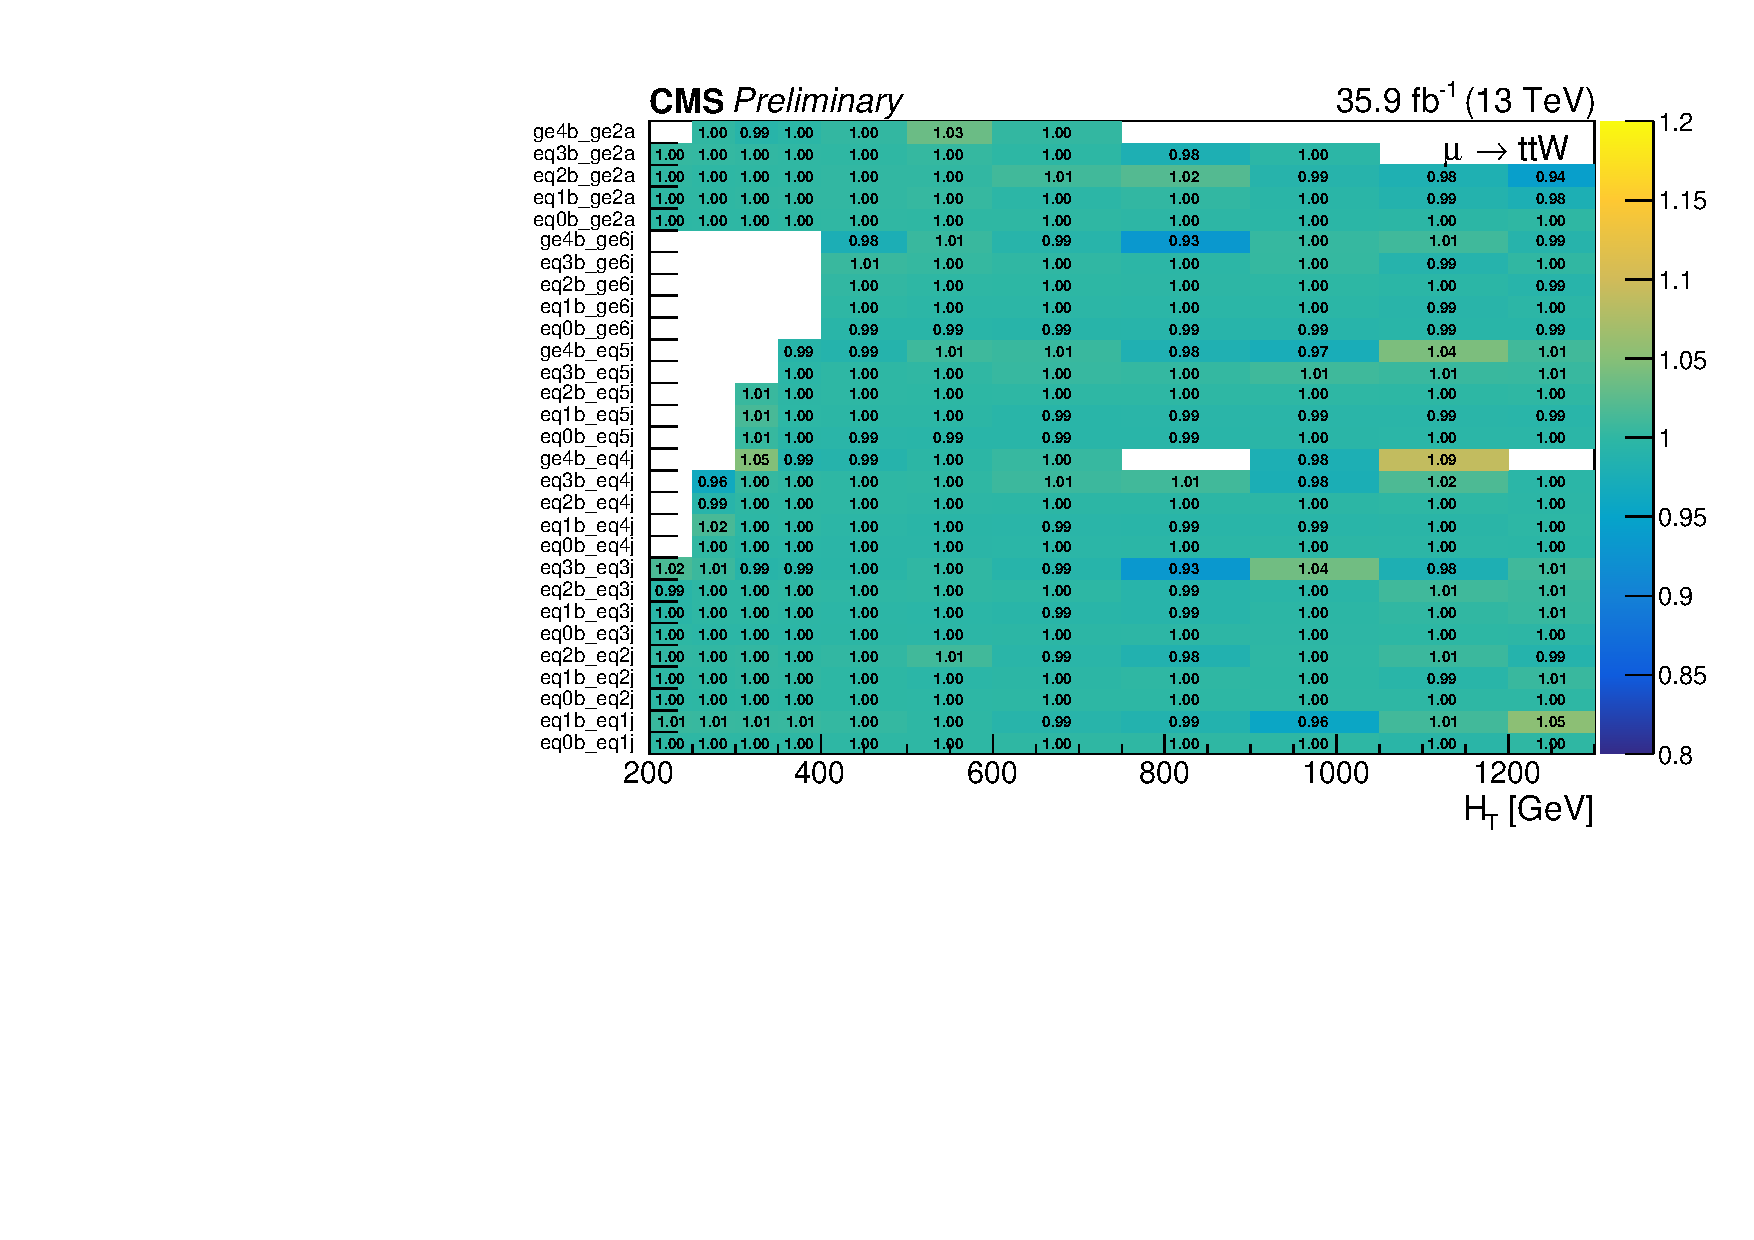
\includegraphics[width=0.5\textwidth]{figs/analysis/transferfactors/tfratio_mu_Ttw_2d_bsfWeightDown}}\\
	\subfloat{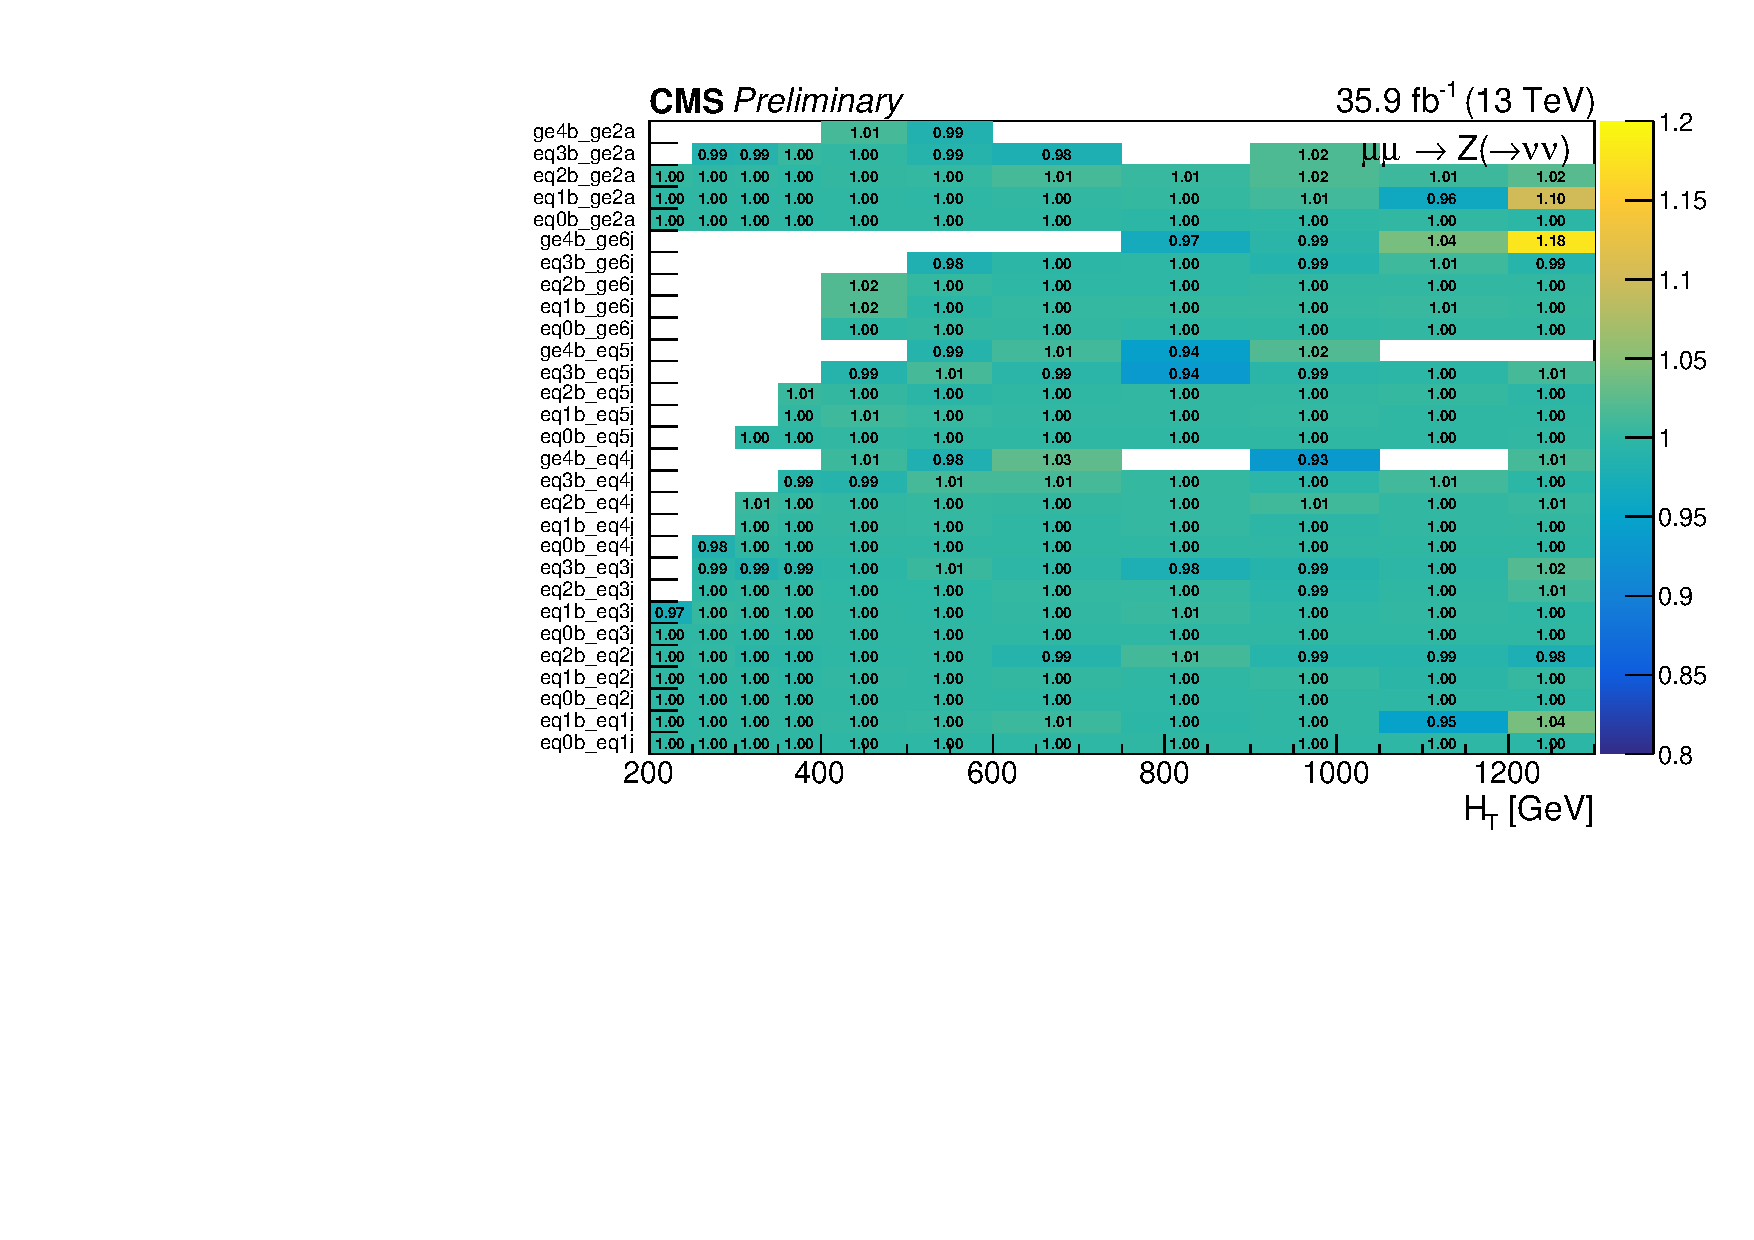
\includegraphics[width=0.5\textwidth]{figs/analysis/transferfactors/tfratio_mumu_Zinv_2d_bsfWeightUp}}~
	\subfloat{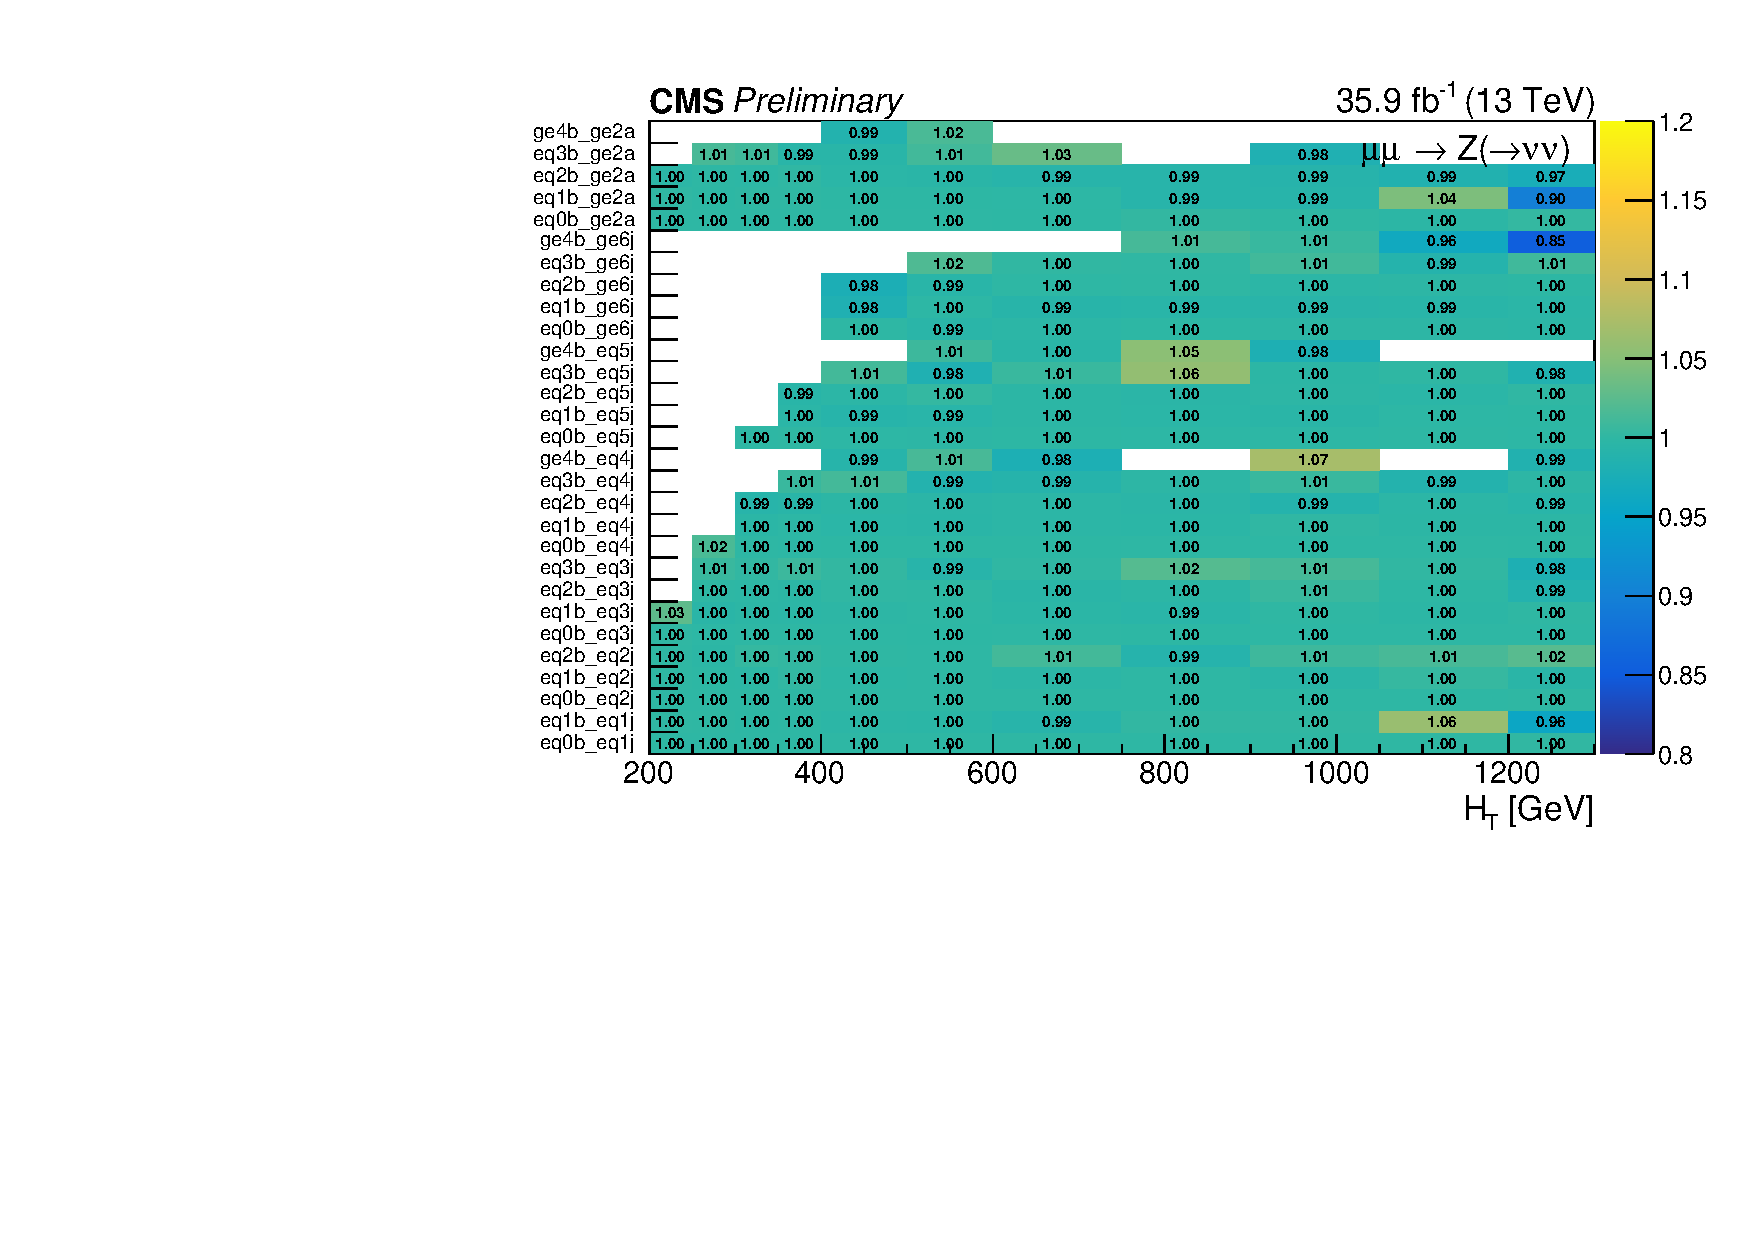
\includegraphics[width=0.5\textwidth]{figs/analysis/transferfactors/tfratio_mumu_Zinv_2d_bsfWeightDown}}\\
	\caption{The ratio of the \Tmutottw (top) and \Tmumutoz (bottom) transfer 
		factors in each \njnbht bin when varying the b-tagging correction 
		factors for bottom and charm quarks by $+1\sigma$ (left) and $-1\sigma$ 
		(right) with respect to 
		their nominal values.}
	\label{fig:tfvariations-btagging-heavy}
\end{figure}

\begin{figure}[h!]
	\subfloat{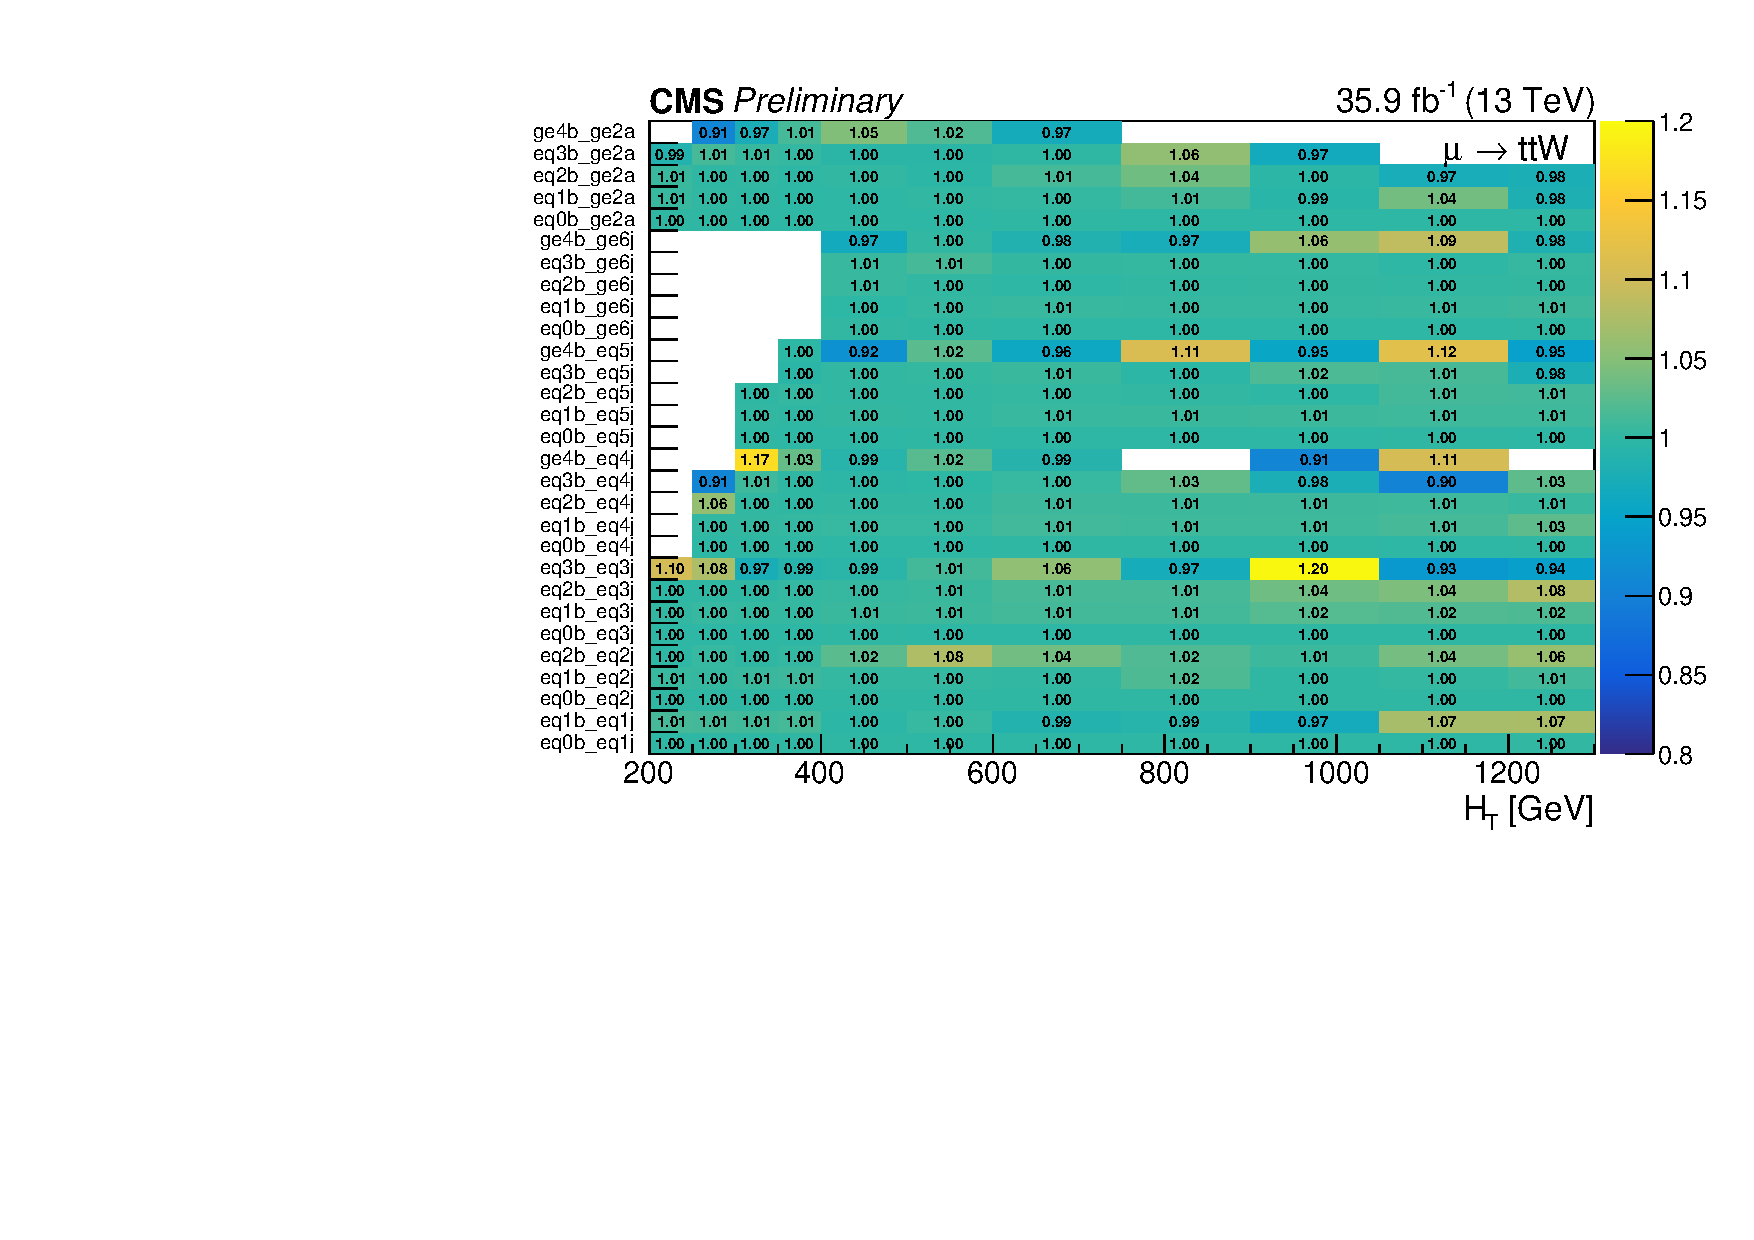
\includegraphics[width=0.5\textwidth]{figs/analysis/transferfactors/tfratio_mu_Ttw_2d_bsfLightWeightUp}}~
	\subfloat{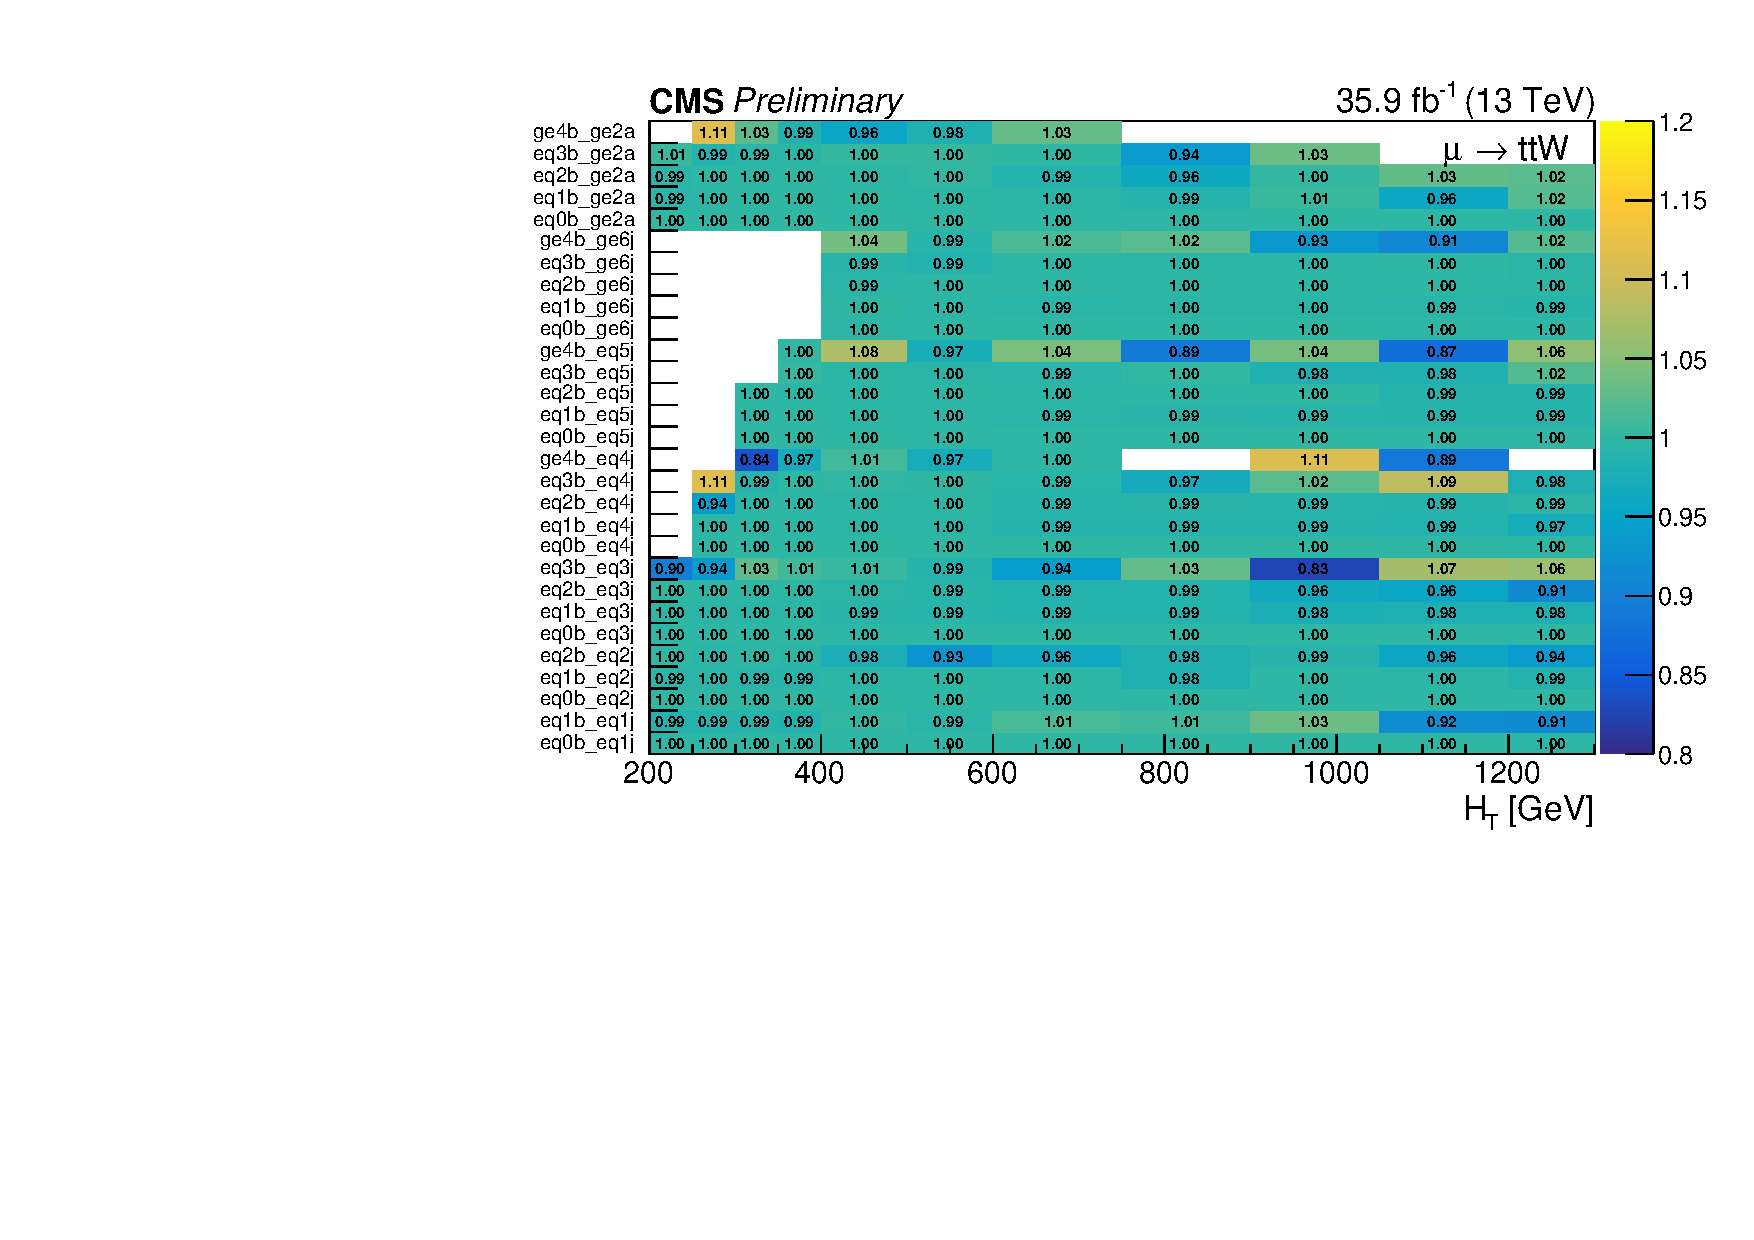
\includegraphics[width=0.5\textwidth]{figs/analysis/transferfactors/tfratio_mu_Ttw_2d_bsfLightWeightDown}}\\
	\subfloat{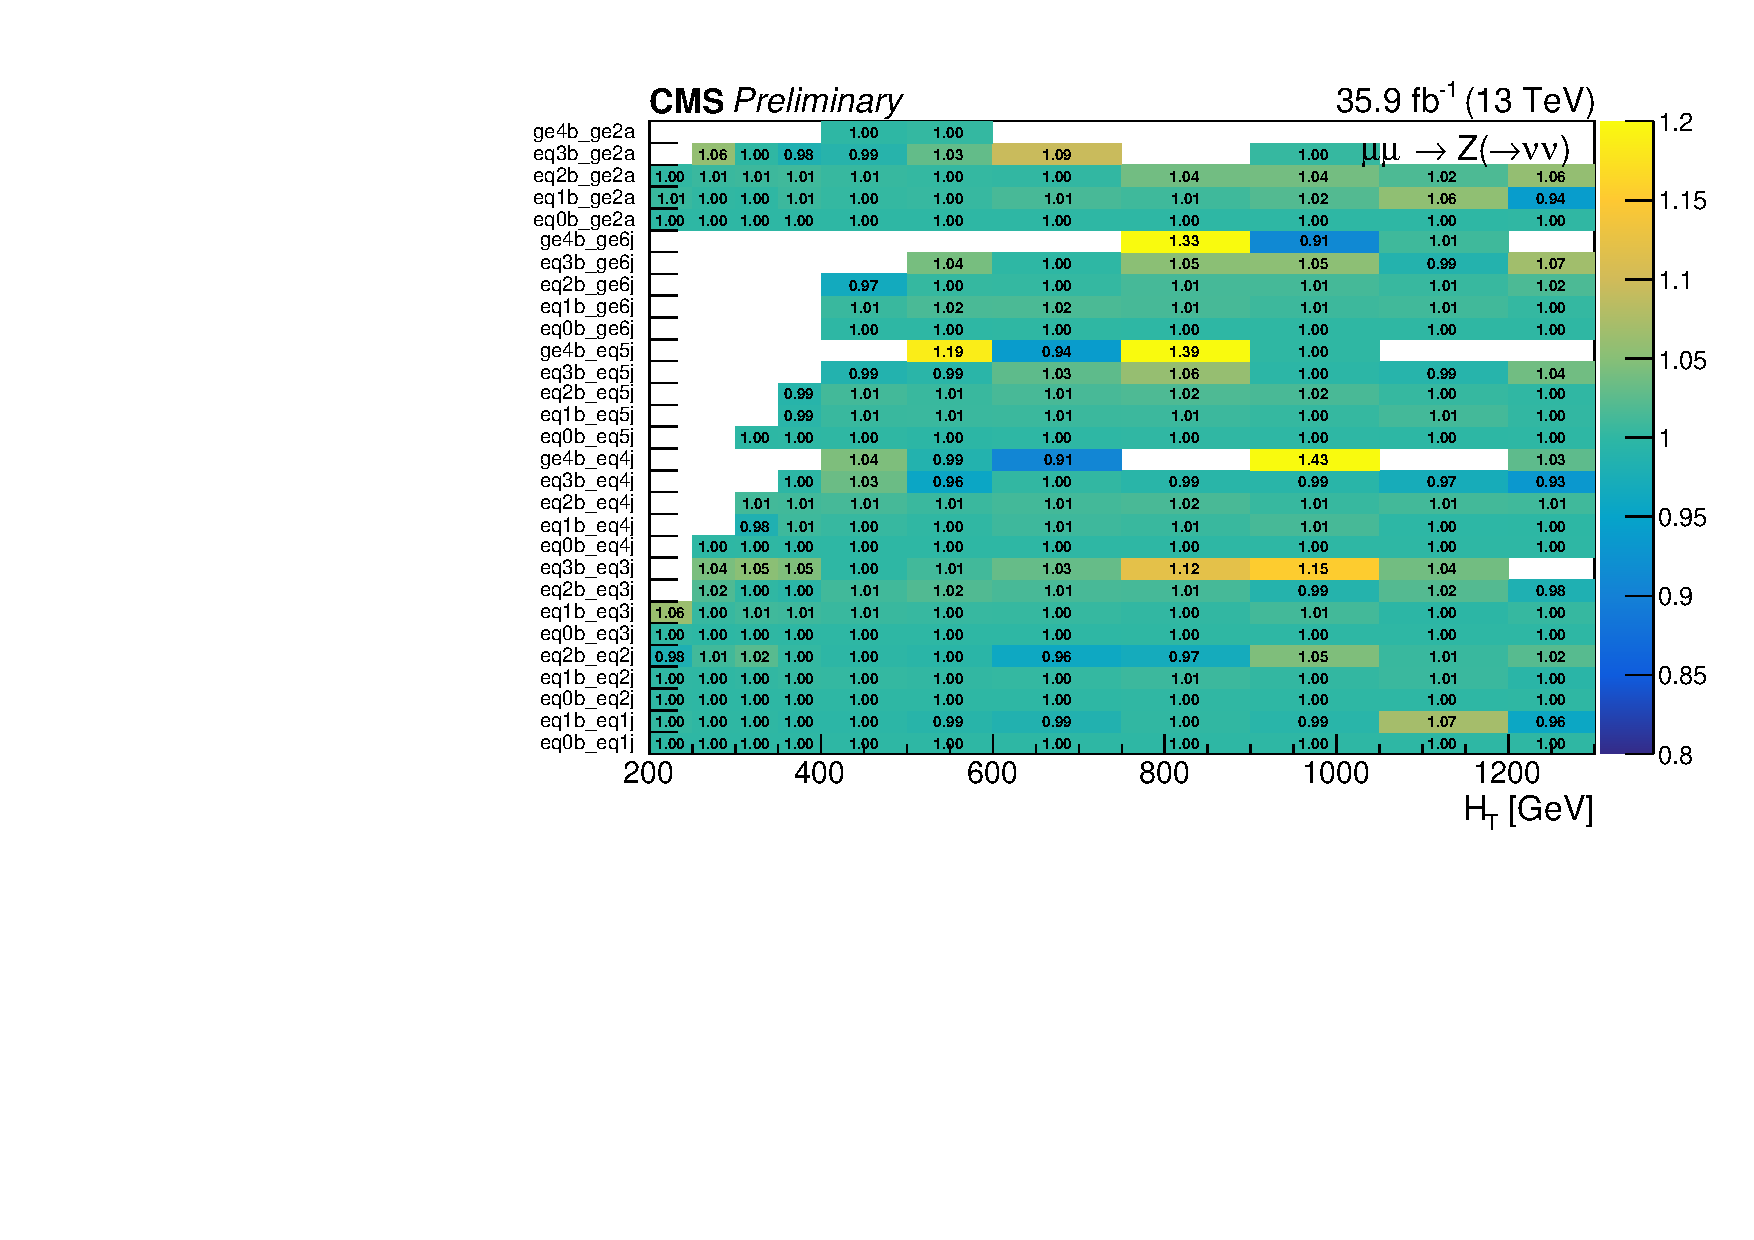
\includegraphics[width=0.5\textwidth]{figs/analysis/transferfactors/tfratio_mumu_Zinv_2d_bsfLightWeightUp}}~
	\subfloat{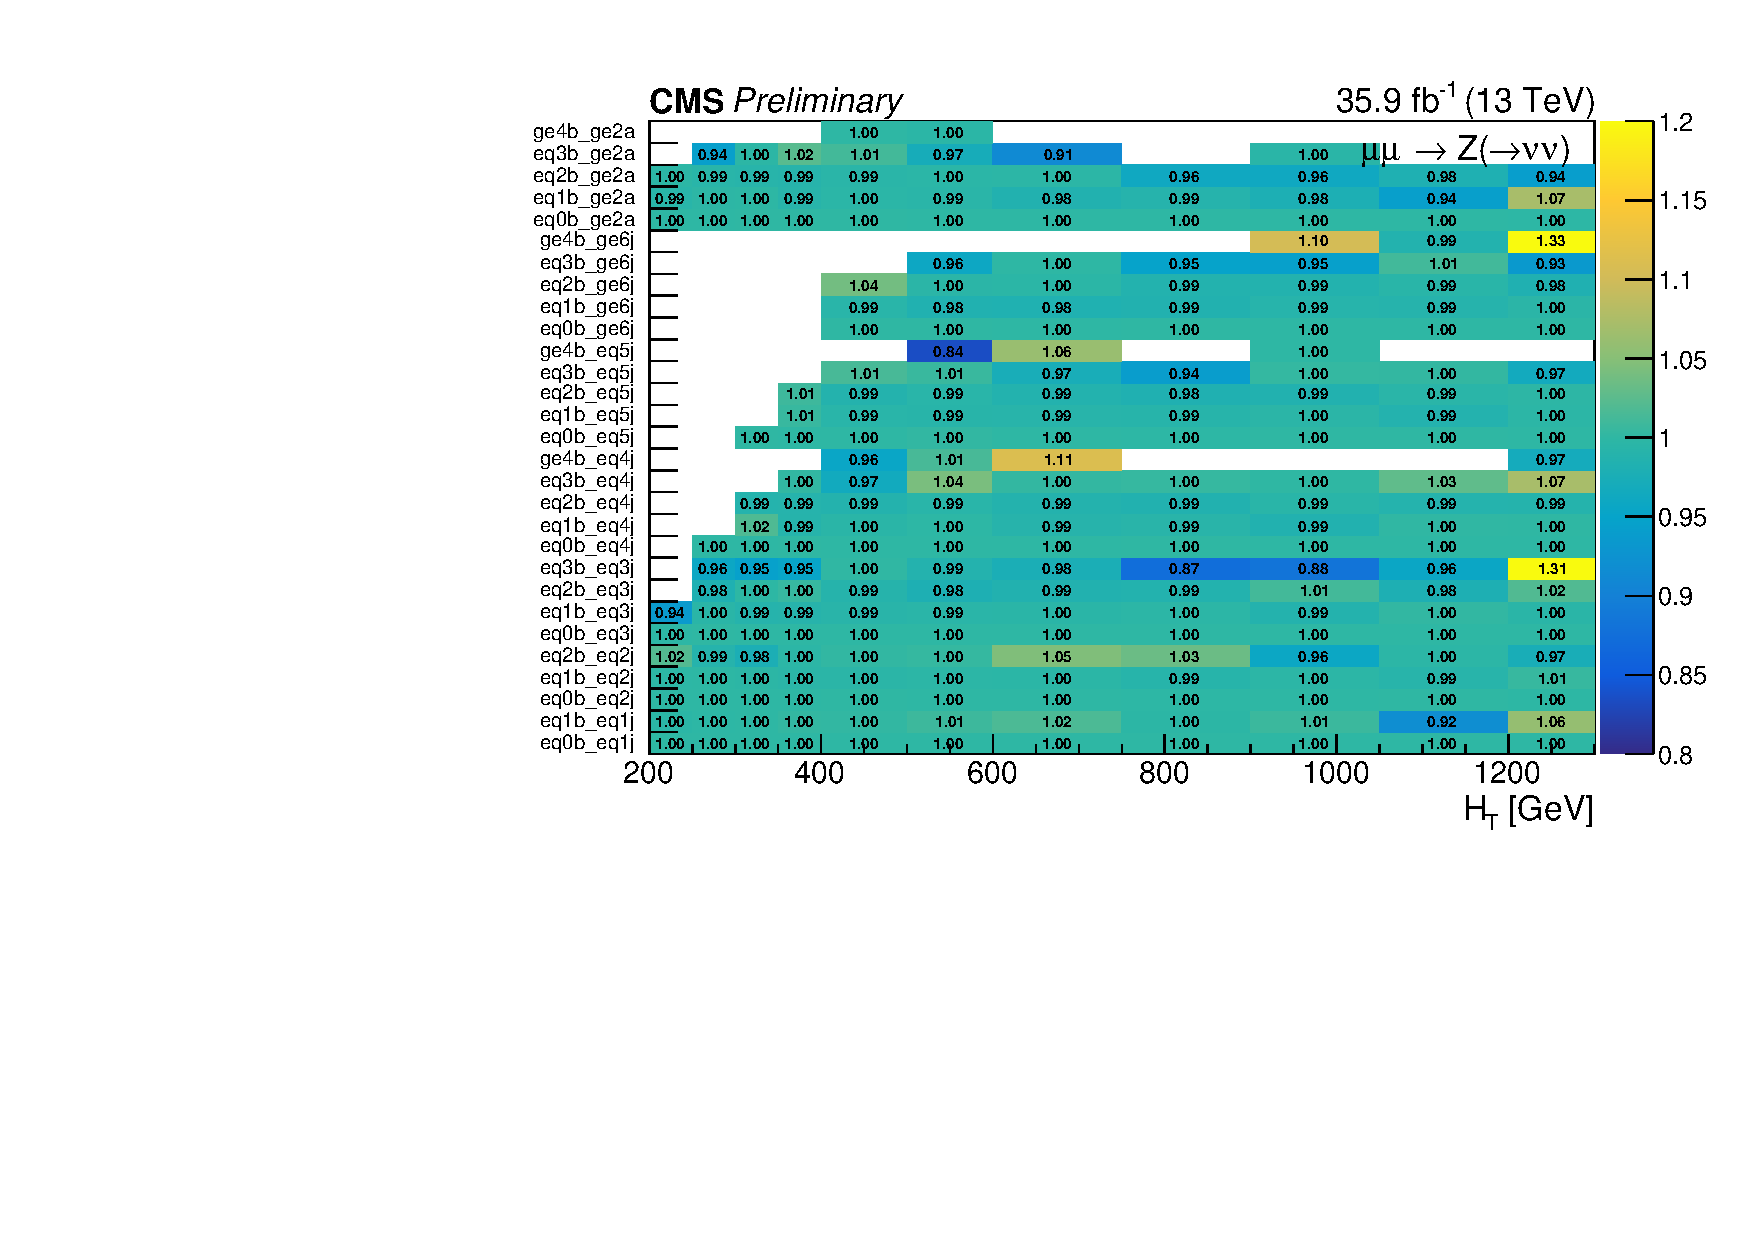
\includegraphics[width=0.5\textwidth]{figs/analysis/transferfactors/tfratio_mumu_Zinv_2d_bsfLightWeightDown}}\\
	\caption{The ratio of the \Tmutottw (top) and \Tmumutoz (bottom) transfer 
		factors in each \njnbht bin when varying the b-tagging correction 
		factors for light partons (u, d, s, gluon) by $+1\sigma$ (left) and 
		$-1\sigma$ (right) with respect to 
		their nominal values.}
	\label{fig:tfvariations-btagging-light}
\end{figure}

\begin{figure}[h!]
	\subfloat{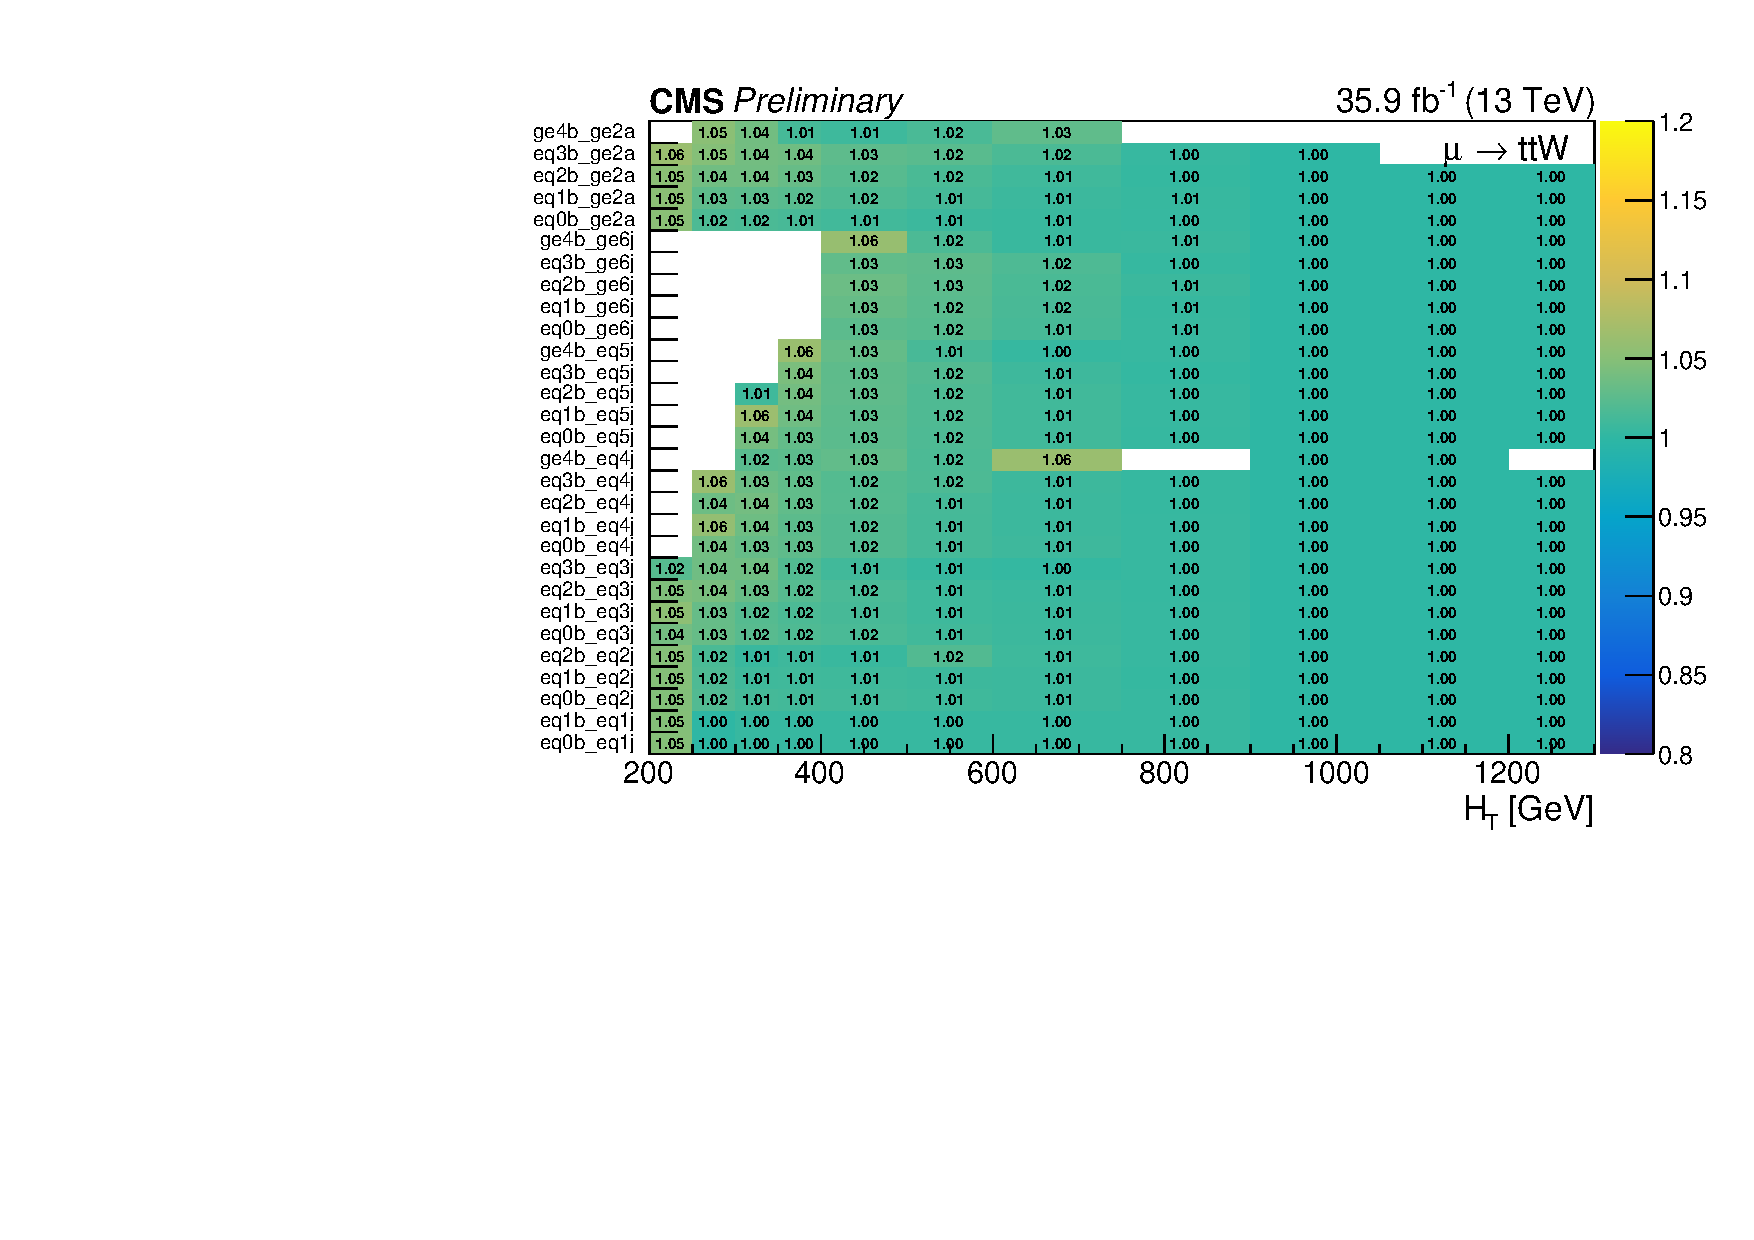
\includegraphics[width=0.5\textwidth]{figs/analysis/transferfactors/tfratio_mu_Ttw_2d_triggerWeightUp}}~
	\subfloat{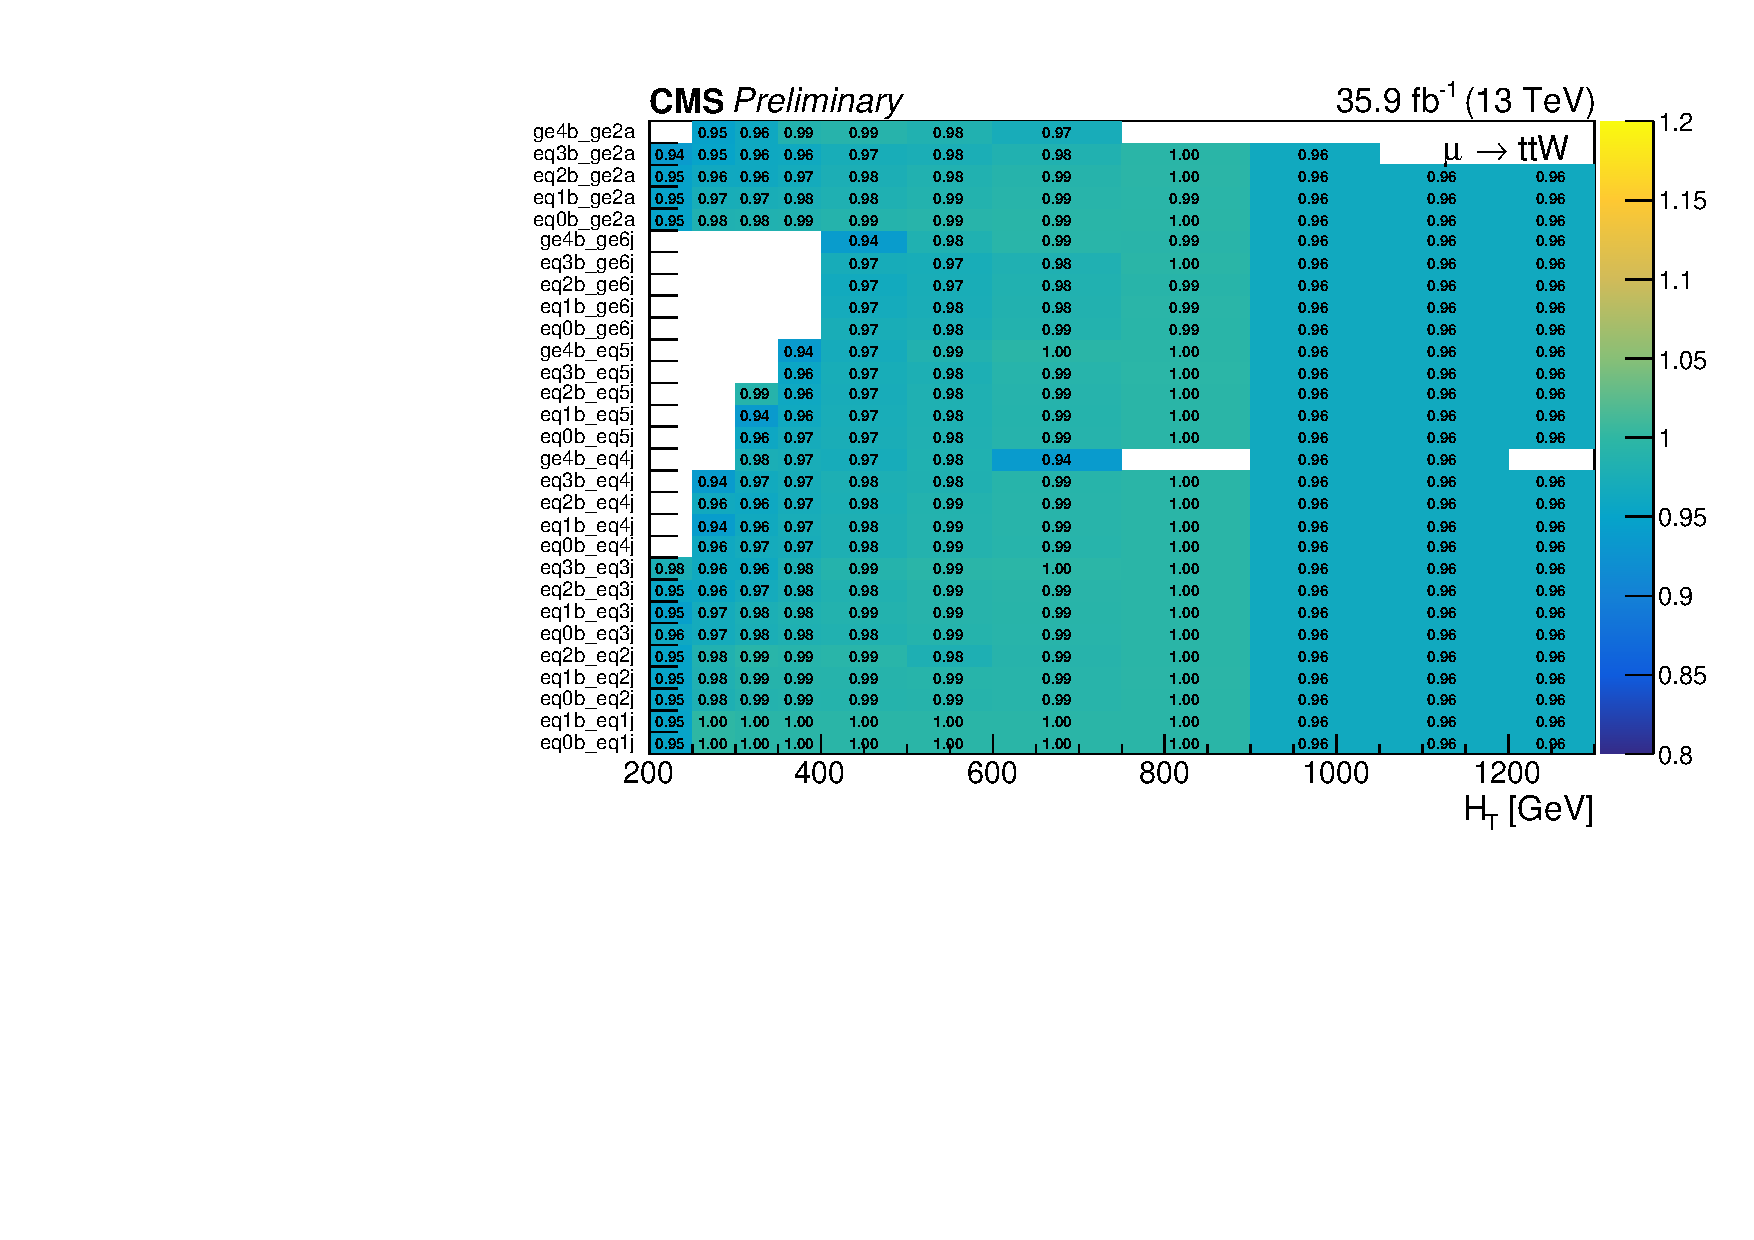
\includegraphics[width=0.5\textwidth]{figs/analysis/transferfactors/tfratio_mu_Ttw_2d_triggerWeightDown}}\\
	\subfloat{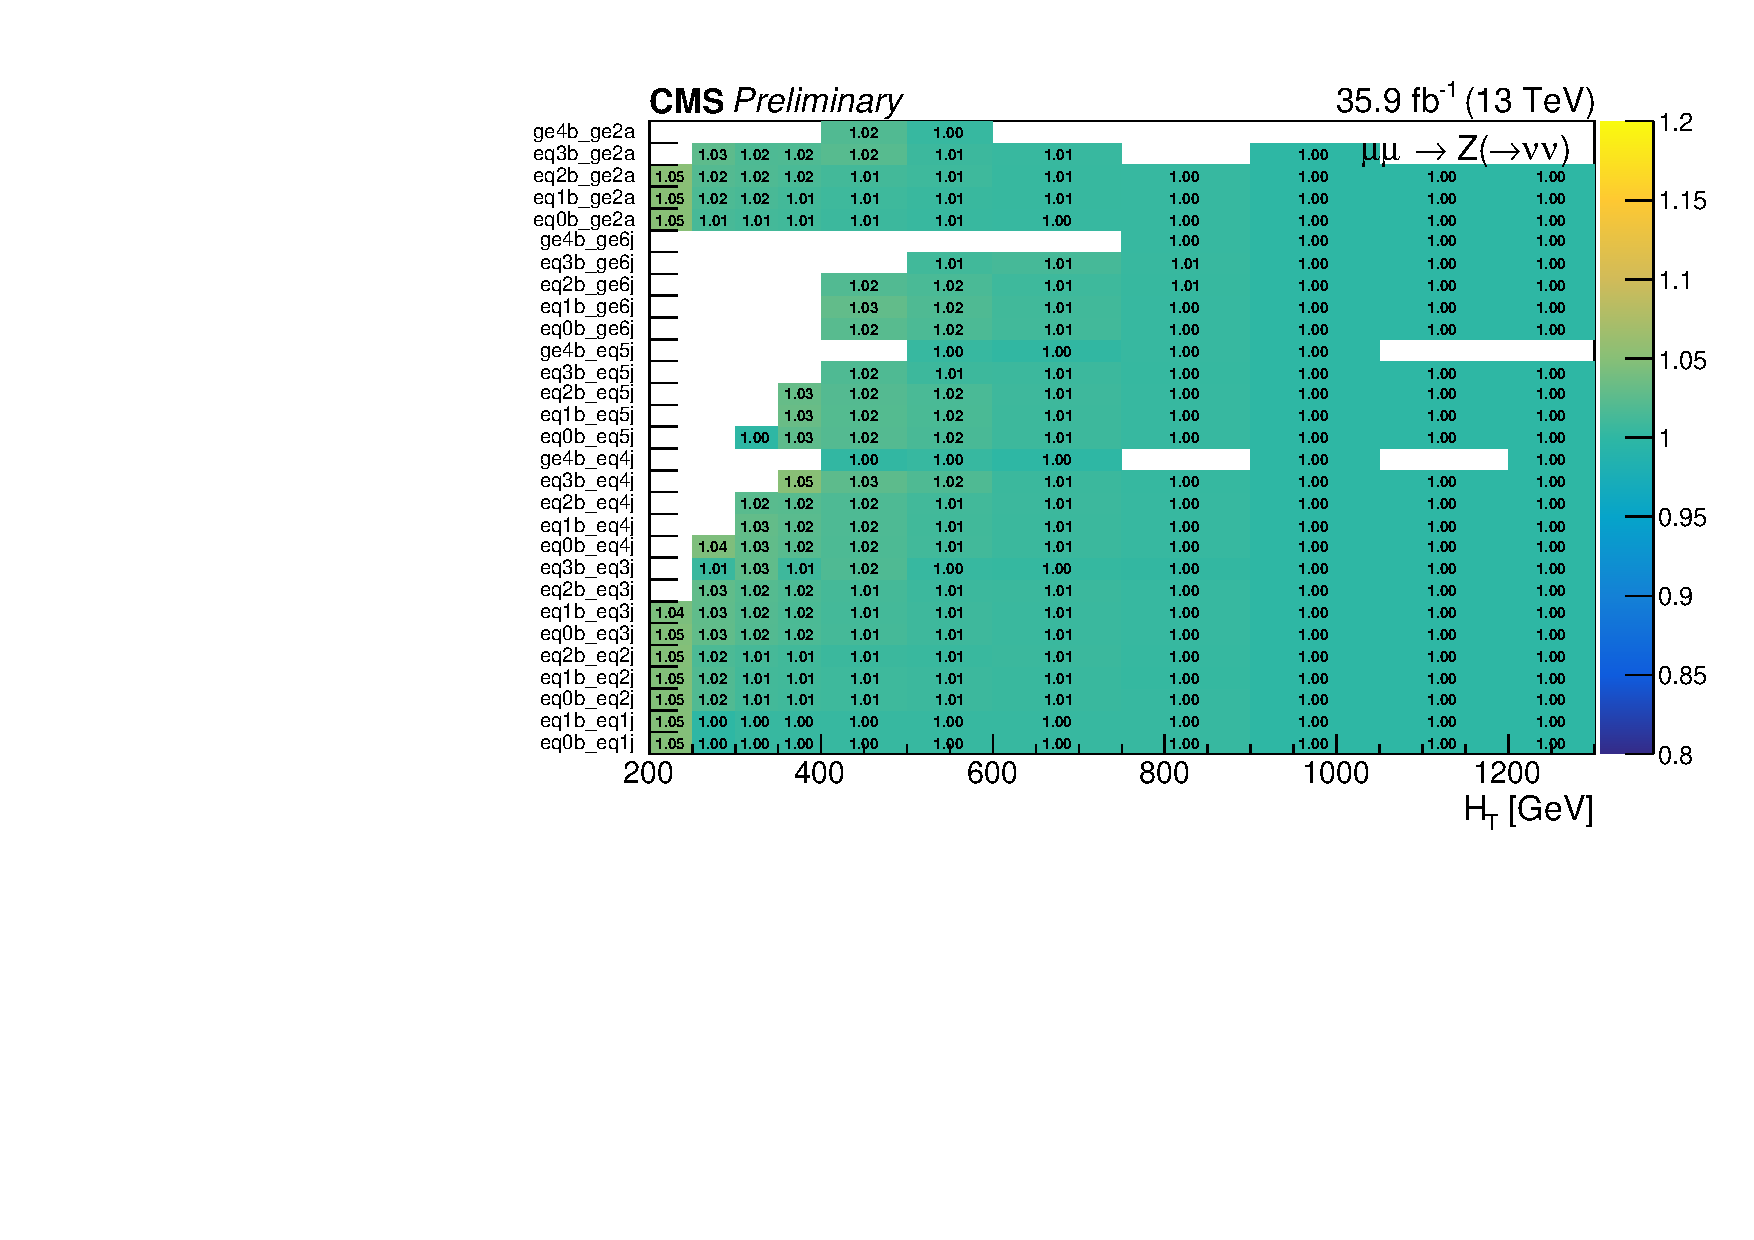
\includegraphics[width=0.5\textwidth]{figs/analysis/transferfactors/tfratio_mumu_Zinv_2d_triggerWeightUp}}~
	\subfloat{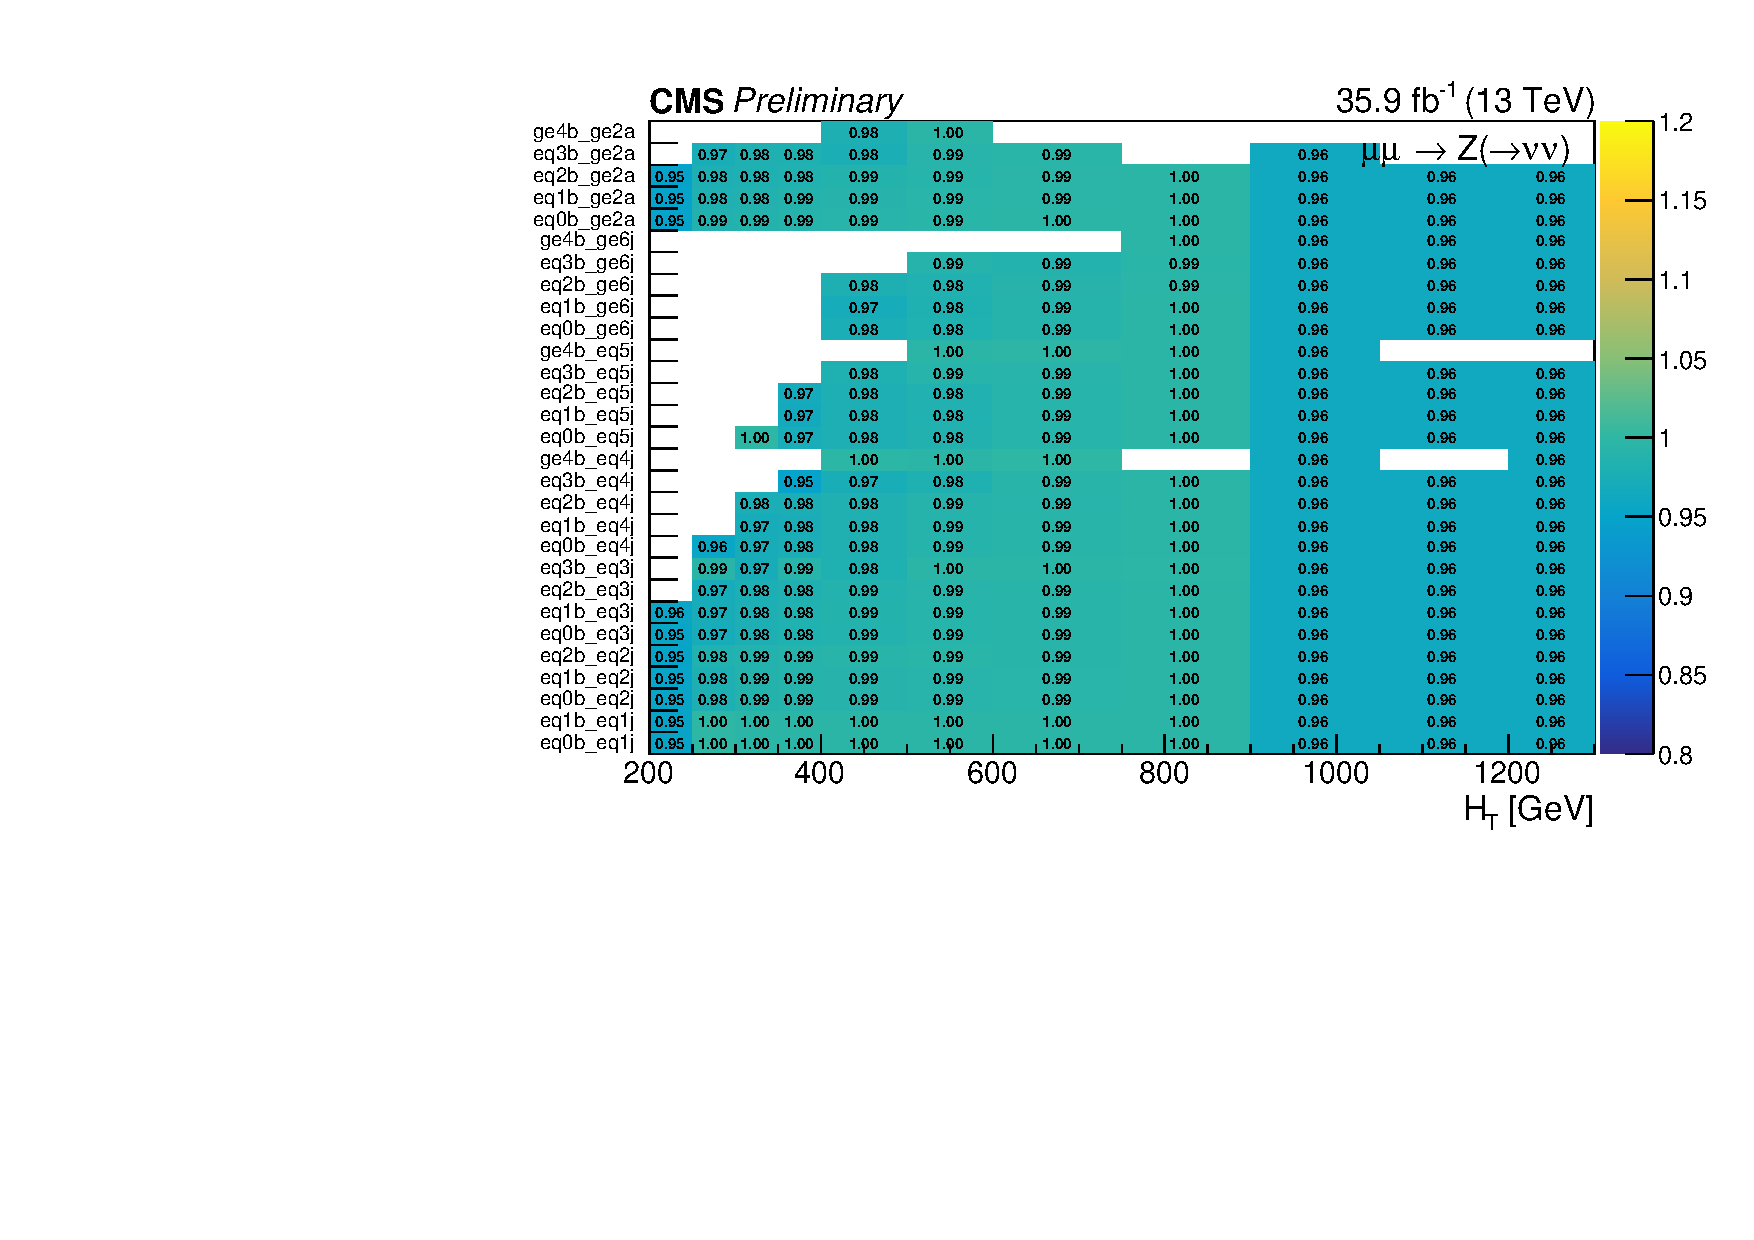
\includegraphics[width=0.5\textwidth]{figs/analysis/transferfactors/tfratio_mumu_Zinv_2d_triggerWeightDown}}\\
	\caption{The ratio of the \Tmutottw (top) and \Tmumutoz (bottom) transfer 
		factors in each \njnbht bin when varying the trigger correction factors 
		by $+1\sigma$ (left) and $-1\sigma$ (right) with respect to 
		their nominal values.}
	\label{fig:tfvariations-trigger}
\end{figure}

\begin{figure}[h!]
	\subfloat{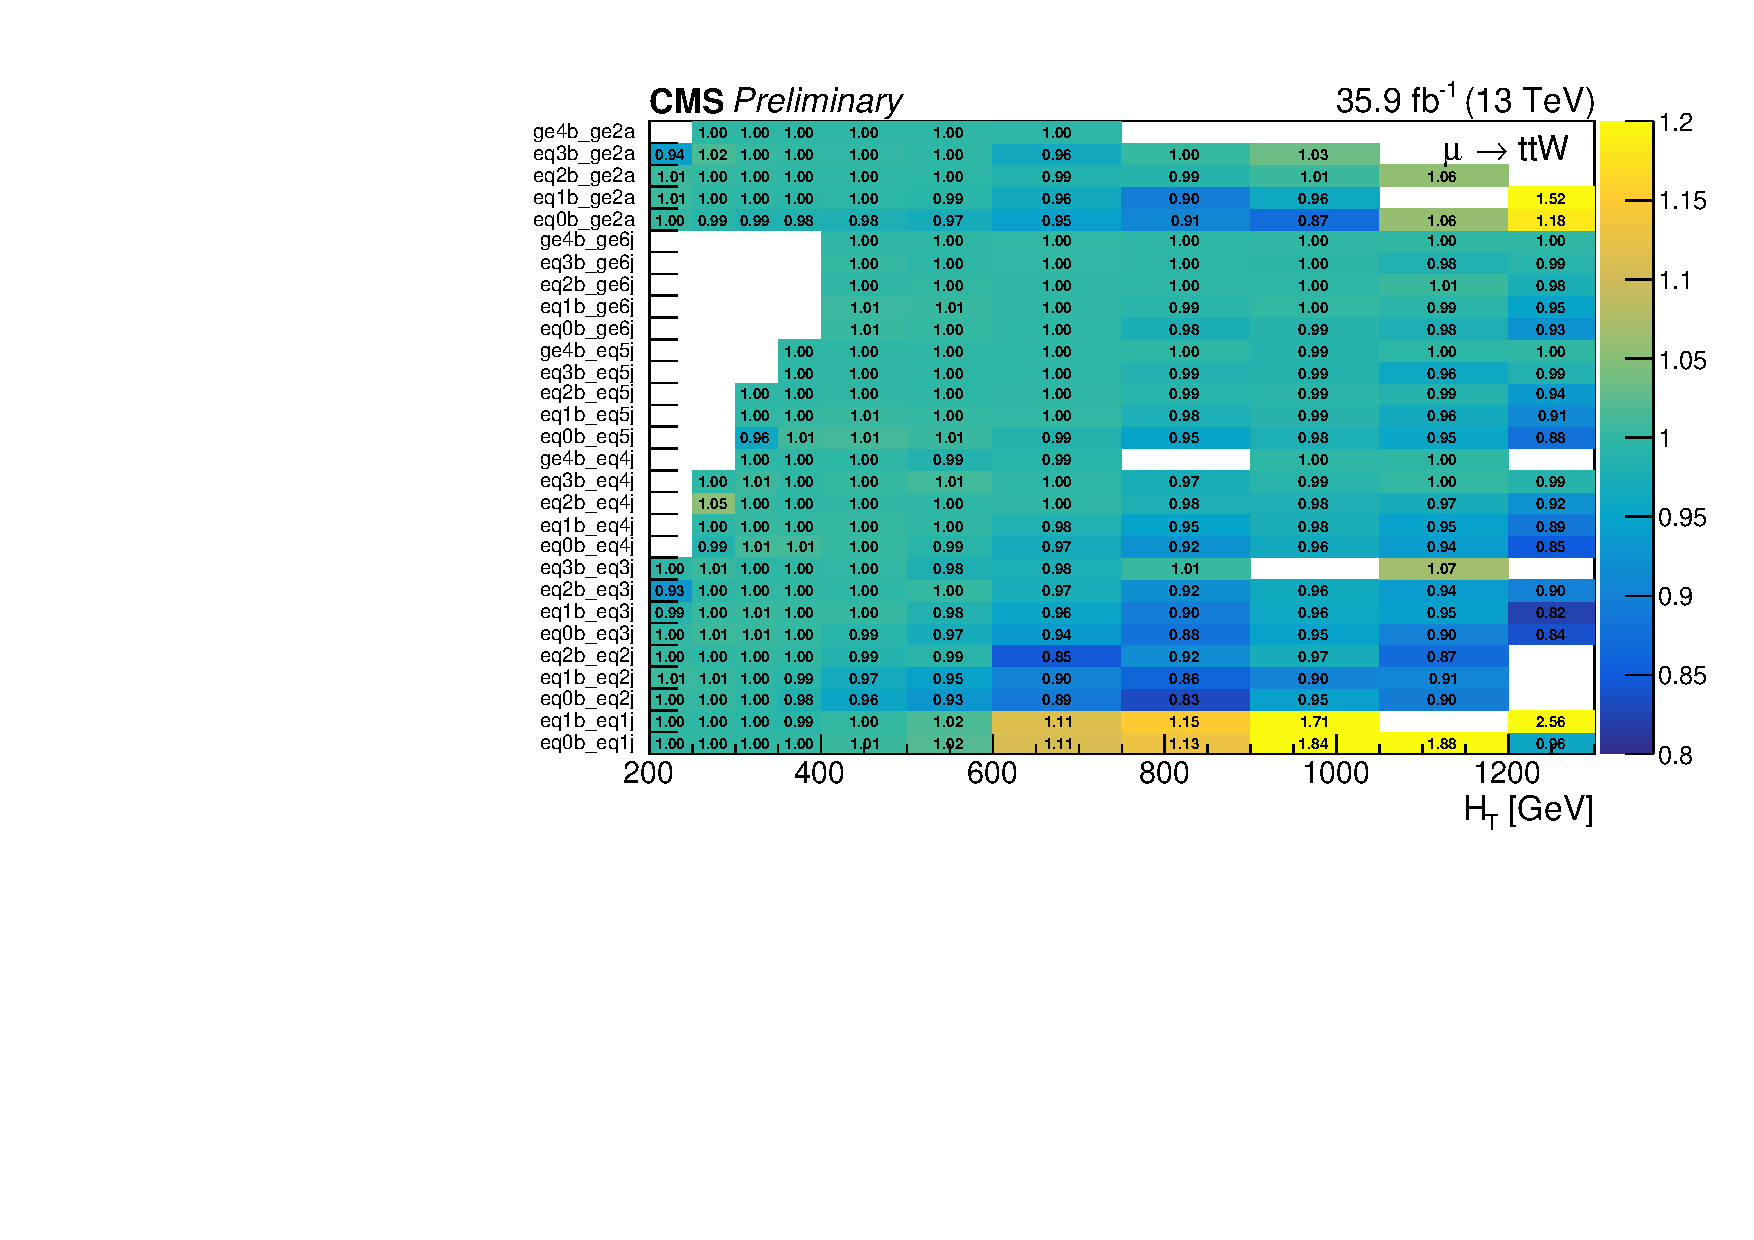
\includegraphics[width=0.5\textwidth]{figs/analysis/transferfactors/tfratio_mu_Ttw_2d_bosonPtWeightUp}}~
	\subfloat{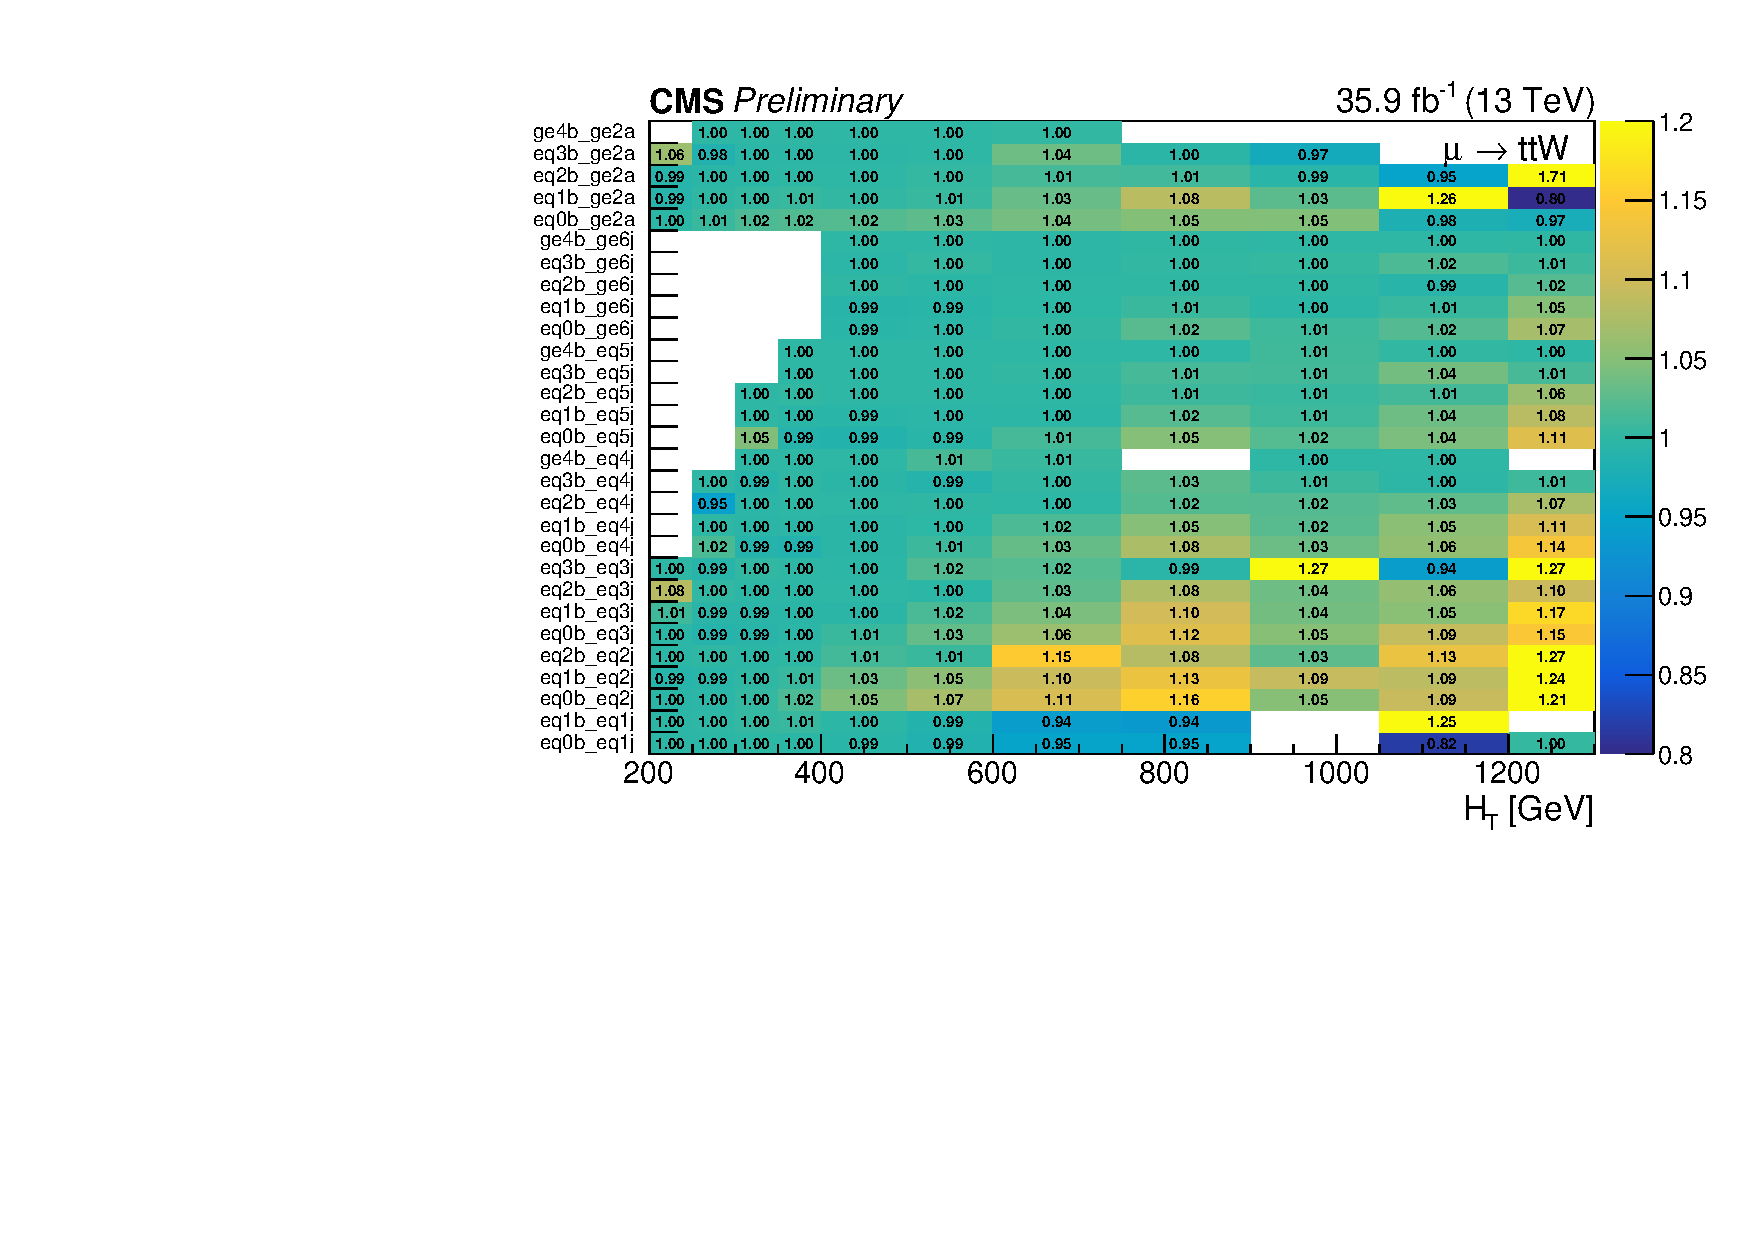
\includegraphics[width=0.5\textwidth]{figs/analysis/transferfactors/tfratio_mu_Ttw_2d_bosonPtWeightDown}}\\
	\subfloat{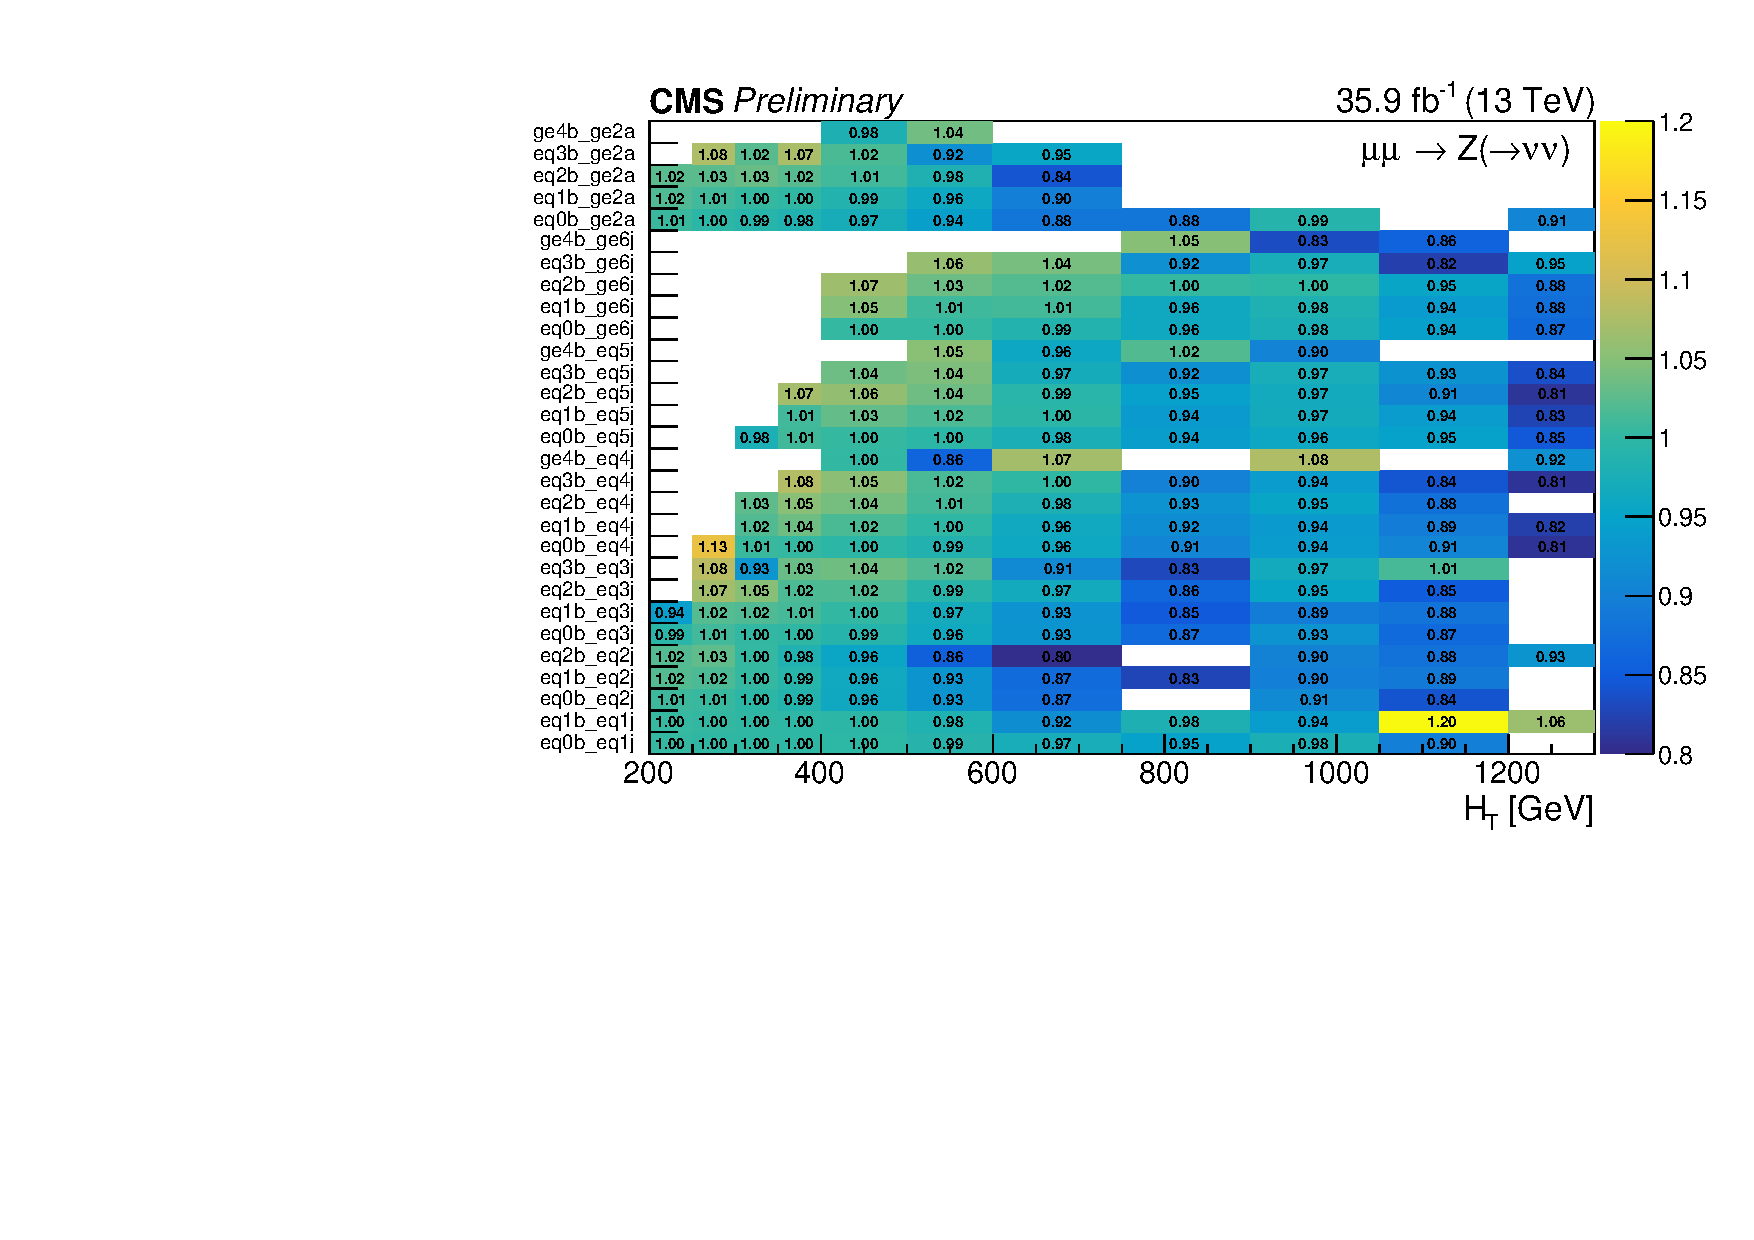
\includegraphics[width=0.5\textwidth]{figs/analysis/transferfactors/tfratio_mumu_Zinv_2d_bosonPtWeightUp}}~
	\subfloat{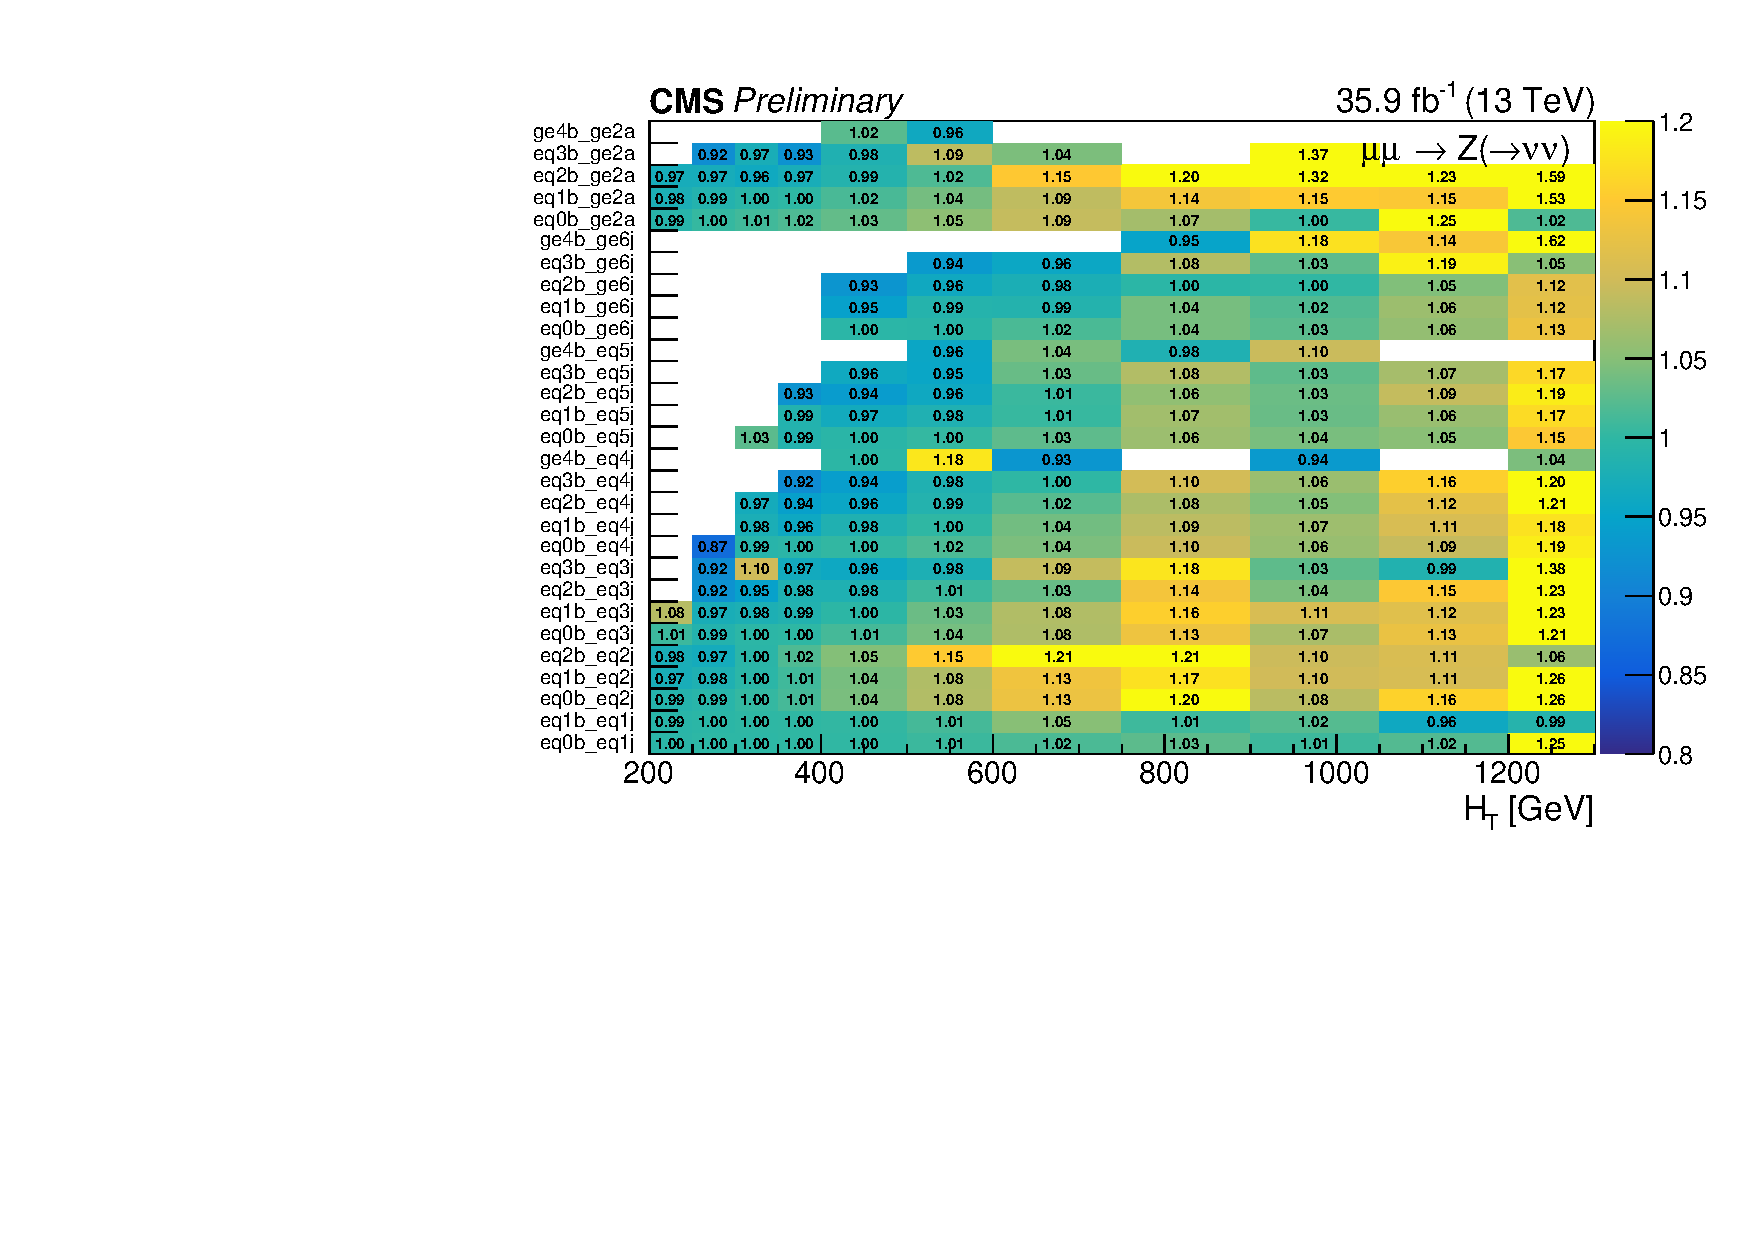
\includegraphics[width=0.5\textwidth]{figs/analysis/transferfactors/tfratio_mumu_Zinv_2d_bosonPtWeightDown}}\\
	\caption{The ratio of the \Tmutottw (top) and \Tmumutoz (bottom) transfer 
		factors in each \njnbht bin when varying the boson \pt dependent NLO 
		correction factors by $+1\sigma$ (left) and $-1\sigma$ (right) with 
		respect to 
		their nominal values.}
	\label{fig:tfvariations-nlo}
\end{figure}

\begin{figure}[h!]
	\subfloat{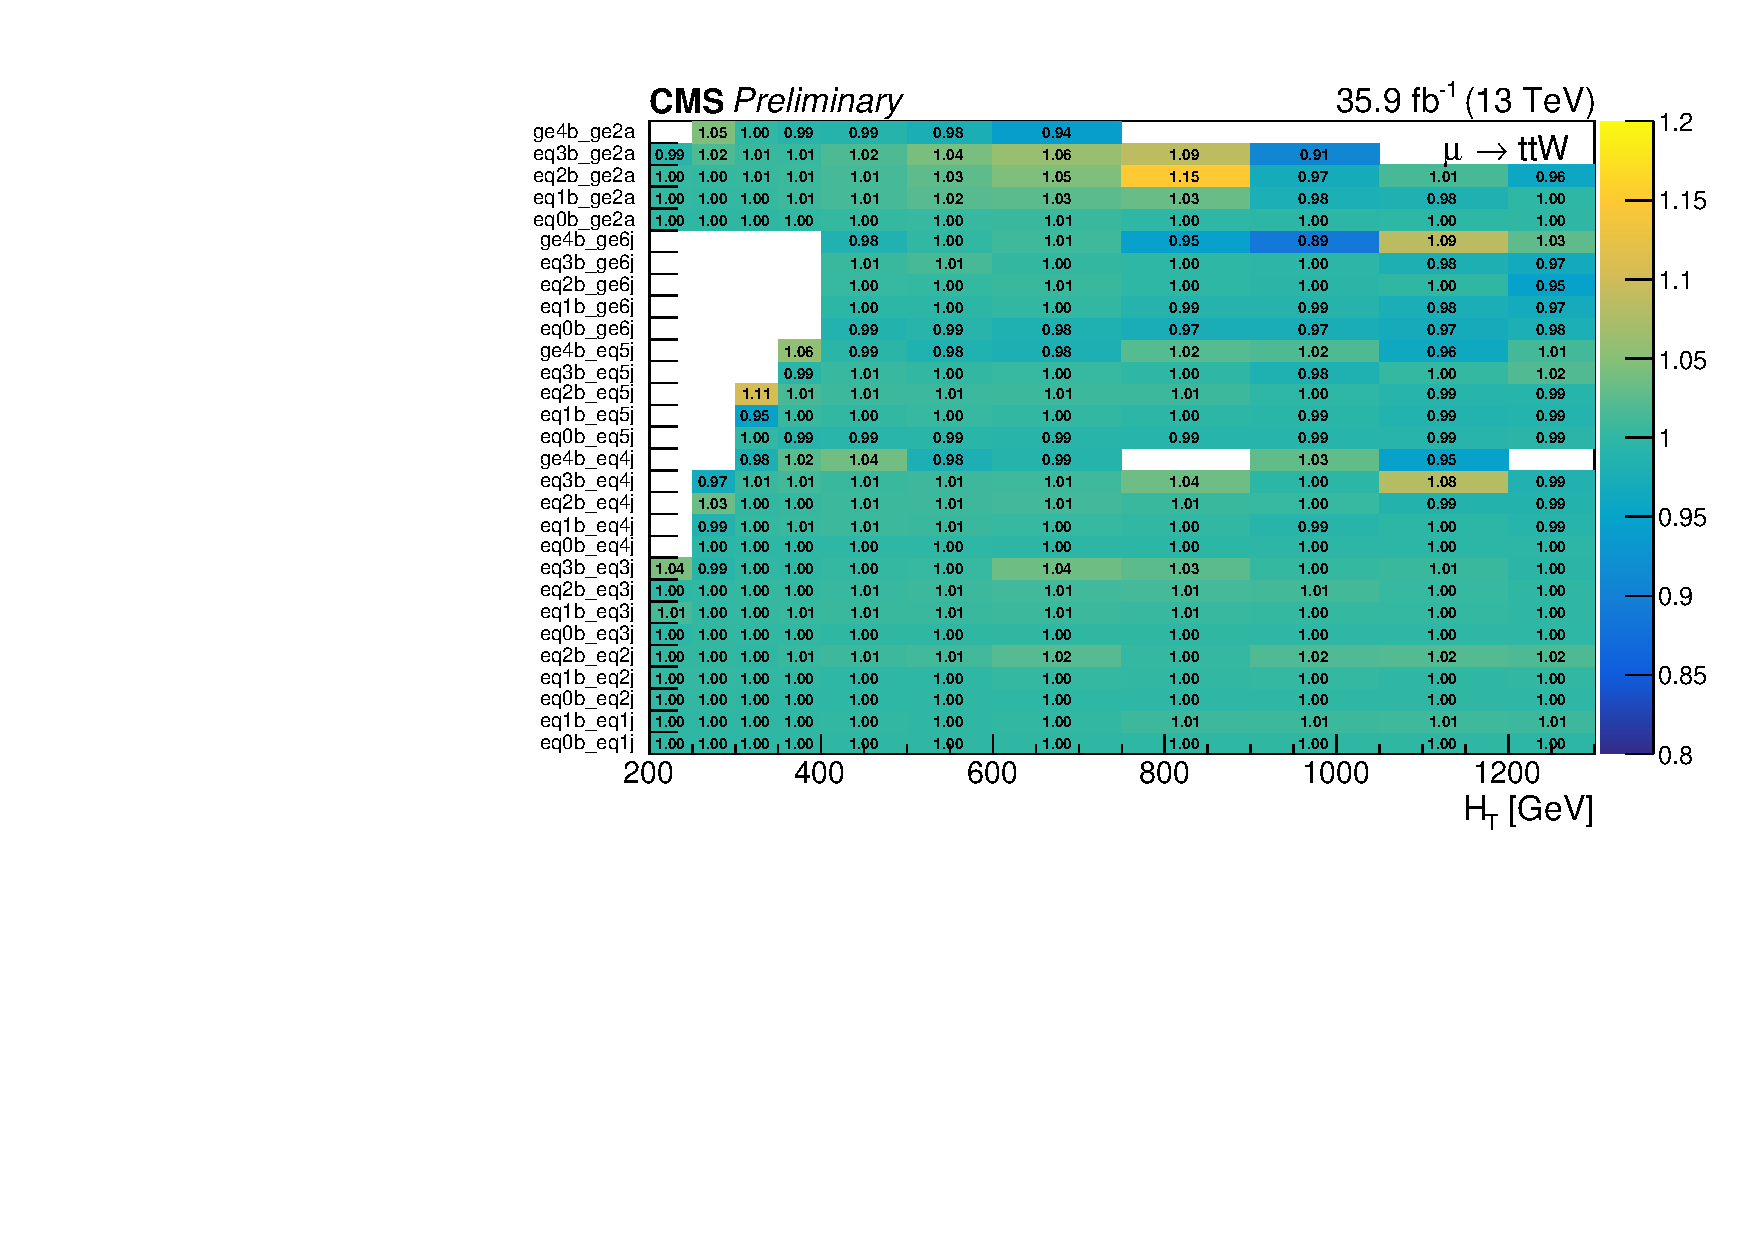
\includegraphics[width=0.5\textwidth]{figs/analysis/transferfactors/tfratio_mu_Ttw_2d_nIsrWeightUp}}~
	\subfloat{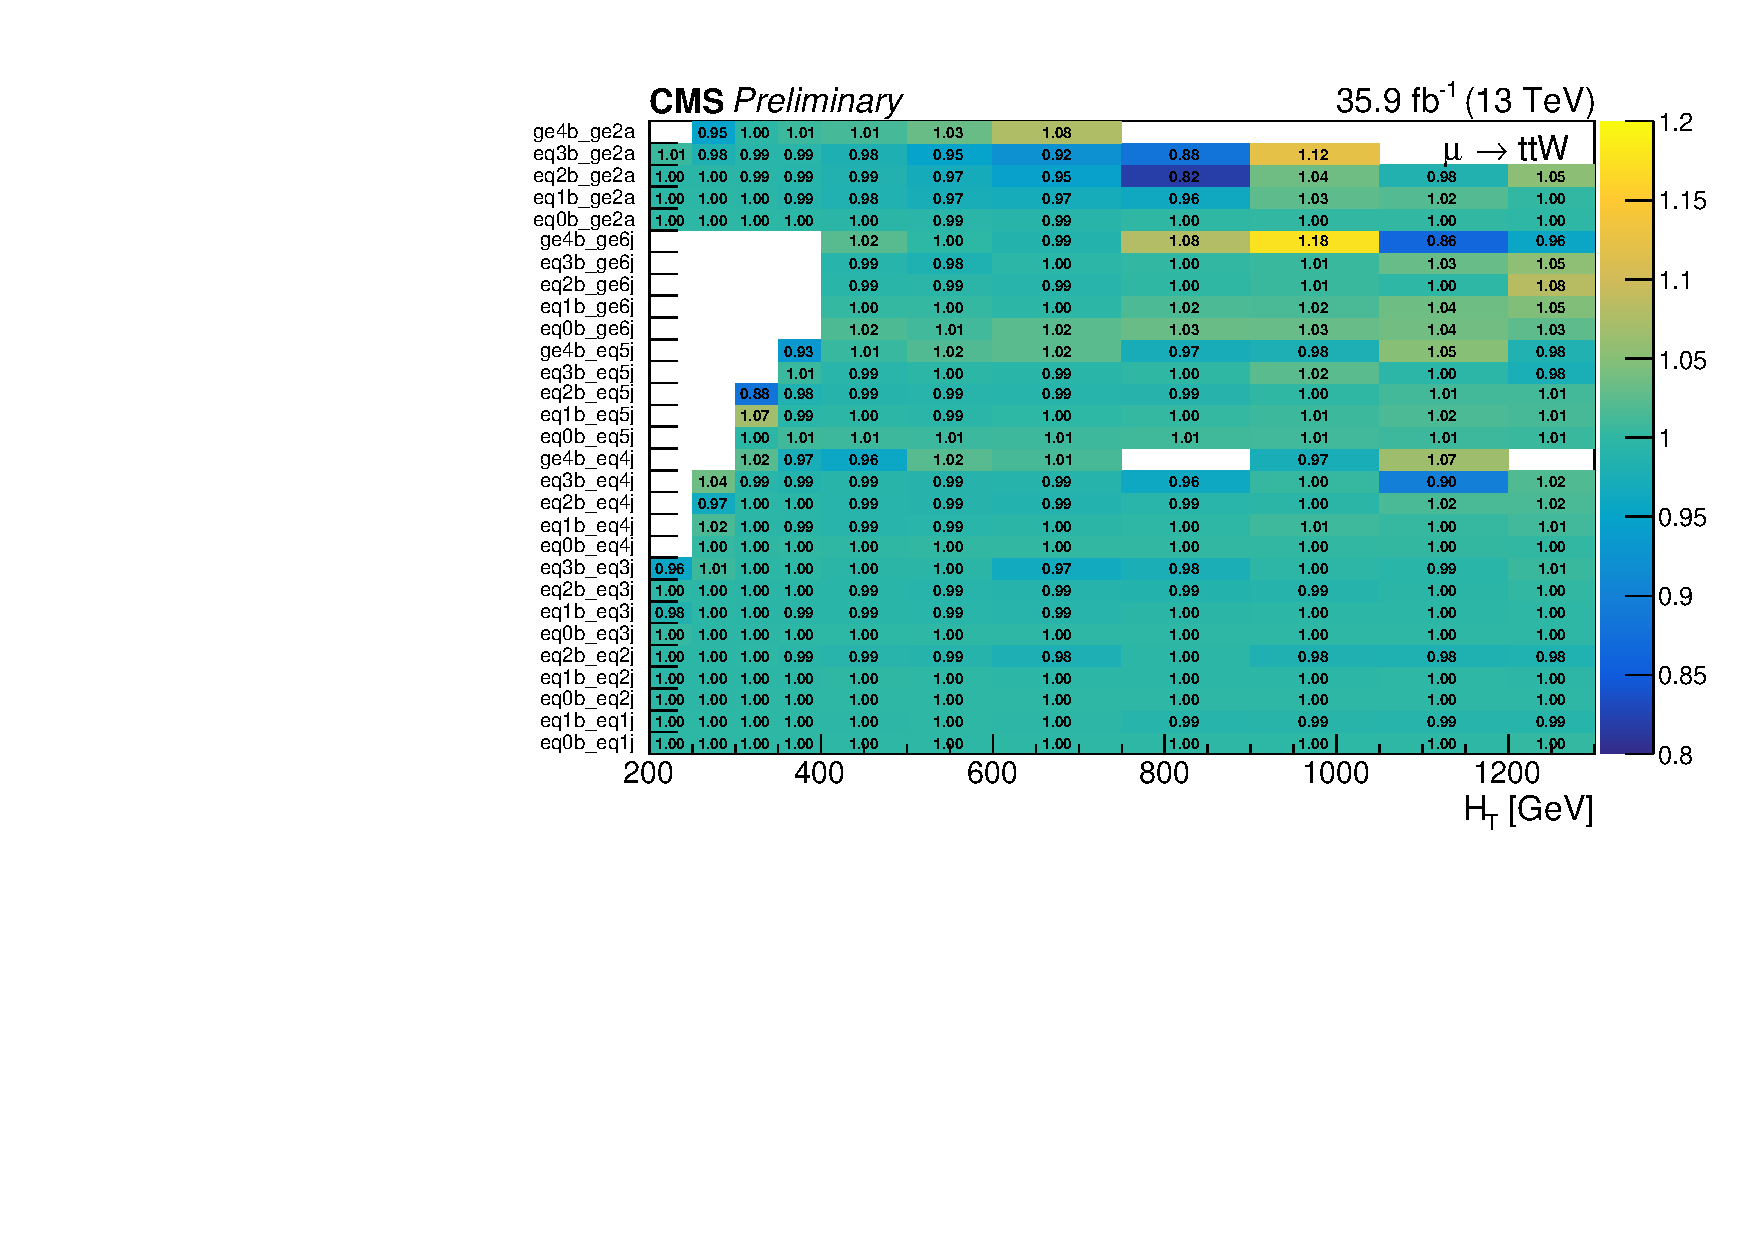
\includegraphics[width=0.5\textwidth]{figs/analysis/transferfactors/tfratio_mu_Ttw_2d_nIsrWeightDown}}\\
	\subfloat{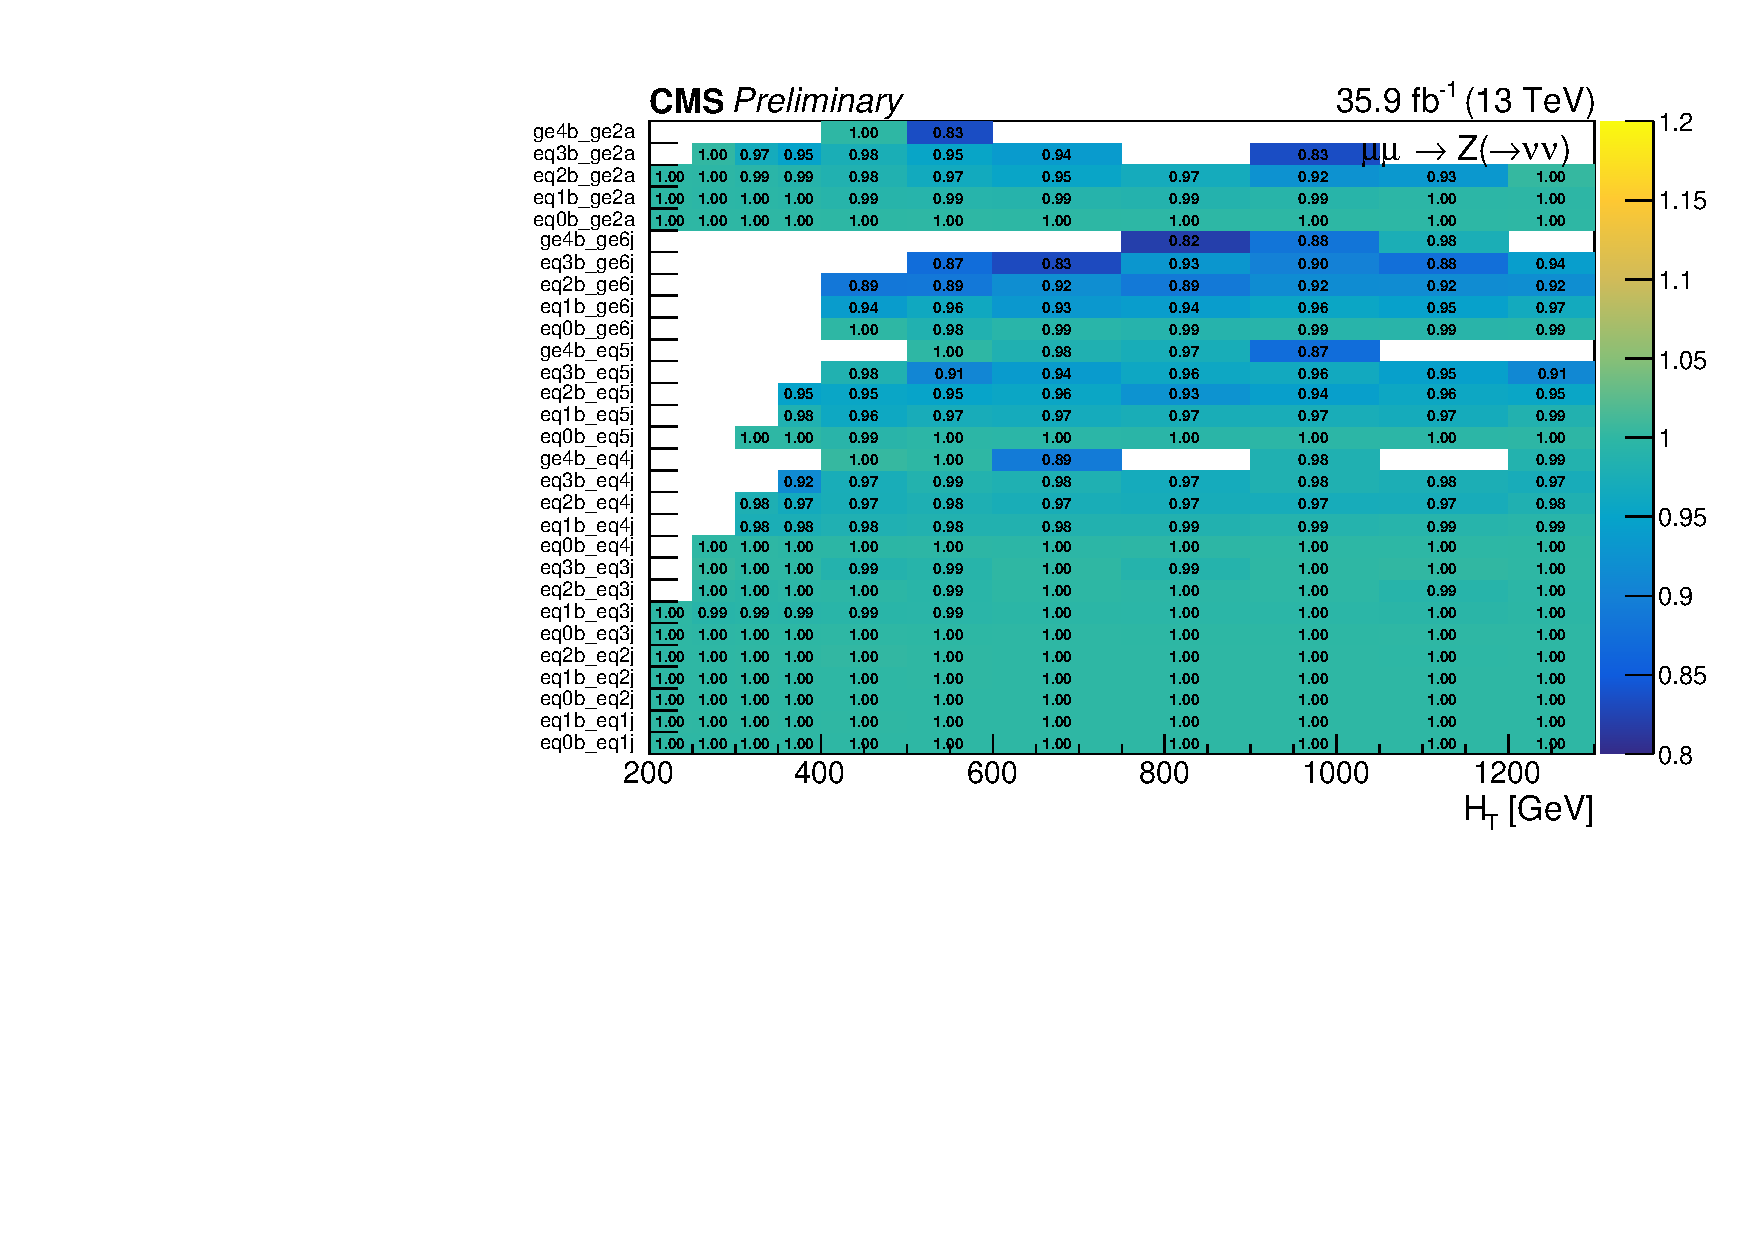
\includegraphics[width=0.5\textwidth]{figs/analysis/transferfactors/tfratio_mumu_Zinv_2d_nIsrWeightUp}}~
	\subfloat{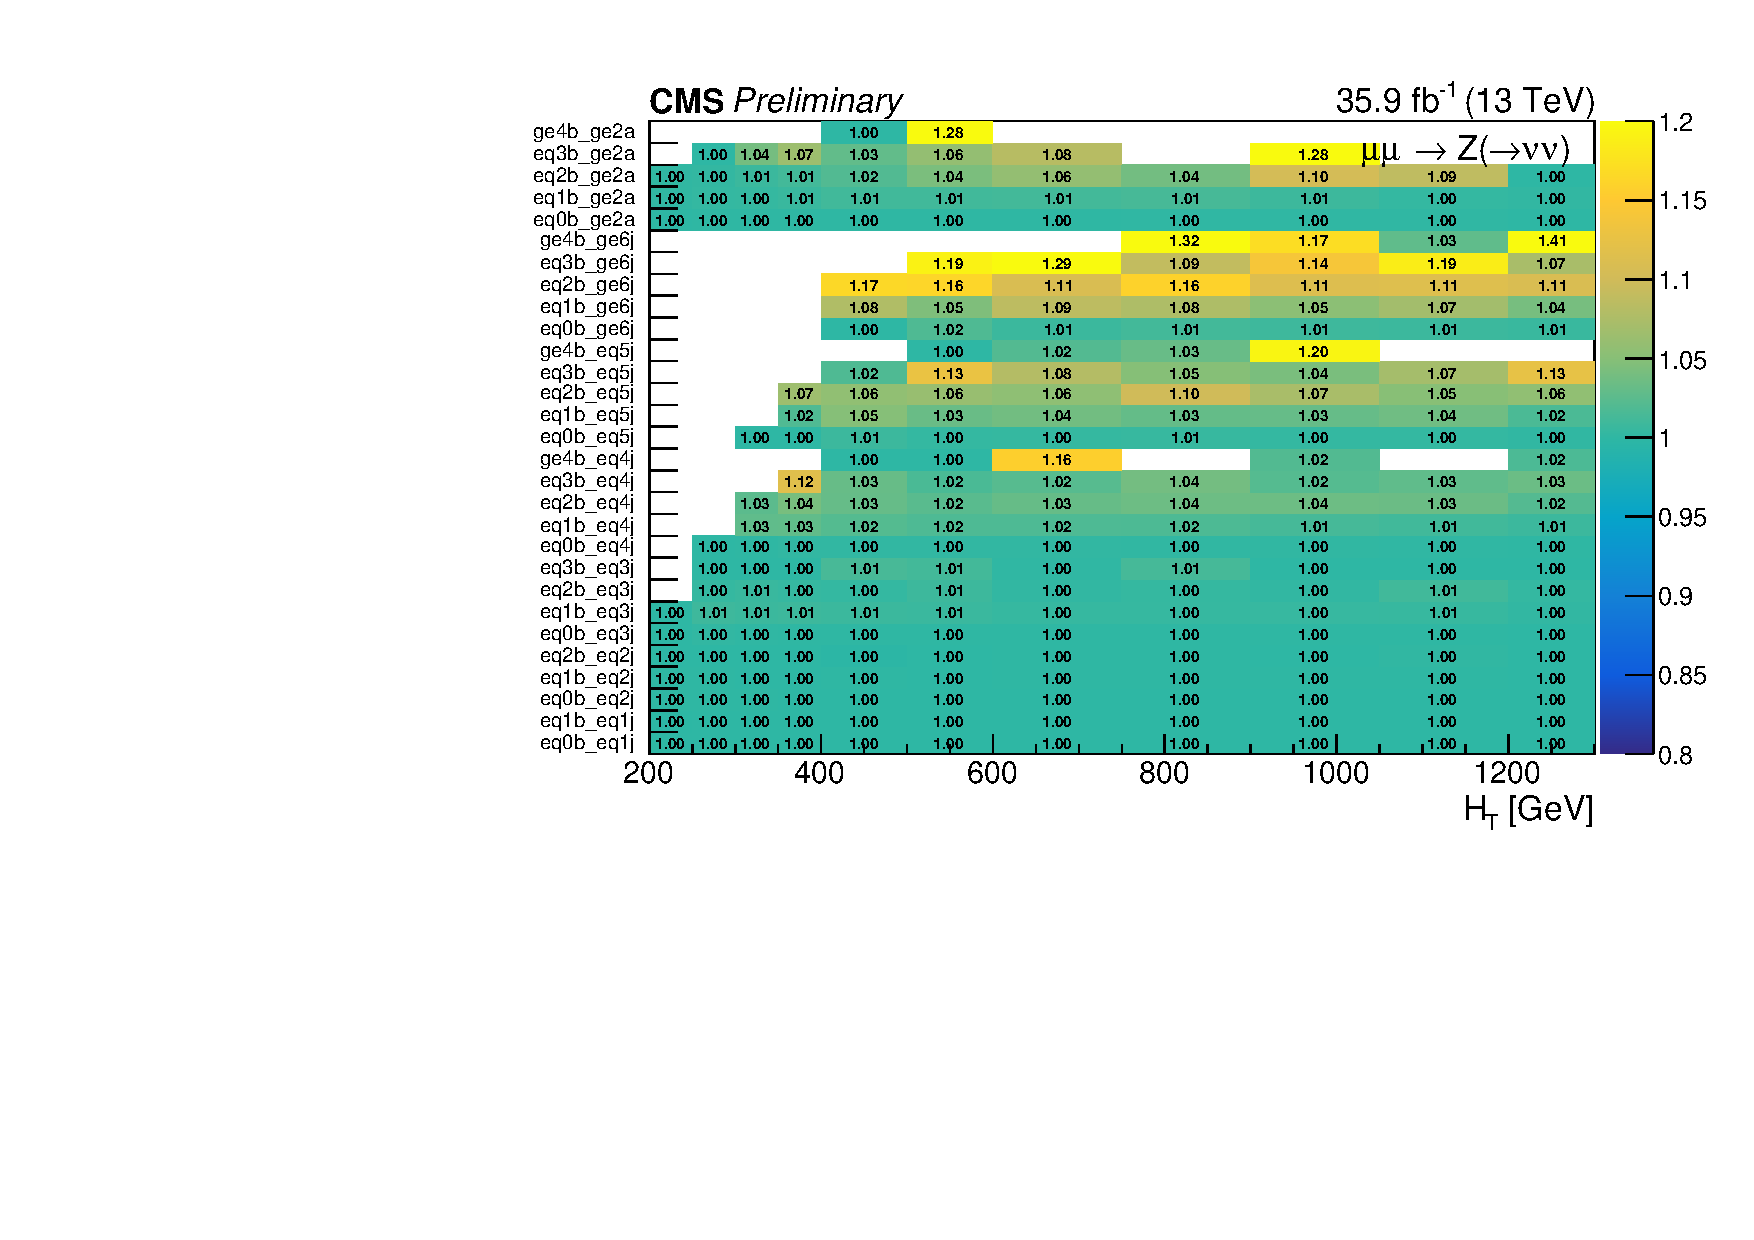
\includegraphics[width=0.5\textwidth]{figs/analysis/transferfactors/tfratio_mumu_Zinv_2d_nIsrWeightDown}}\\
	\caption{The ratio of the \Tmutottw (top) and \Tmumutoz (bottom) transfer 
		factors in each \njnbht bin when varying the \ttbar ISR correction 
		factors by $+1\sigma$ (left) and $-1\sigma$ (right) with respect to 
		their nominal values.}
	\label{fig:tfvariations-nisr}
\end{figure}

\begin{figure}[h!]
	\subfloat{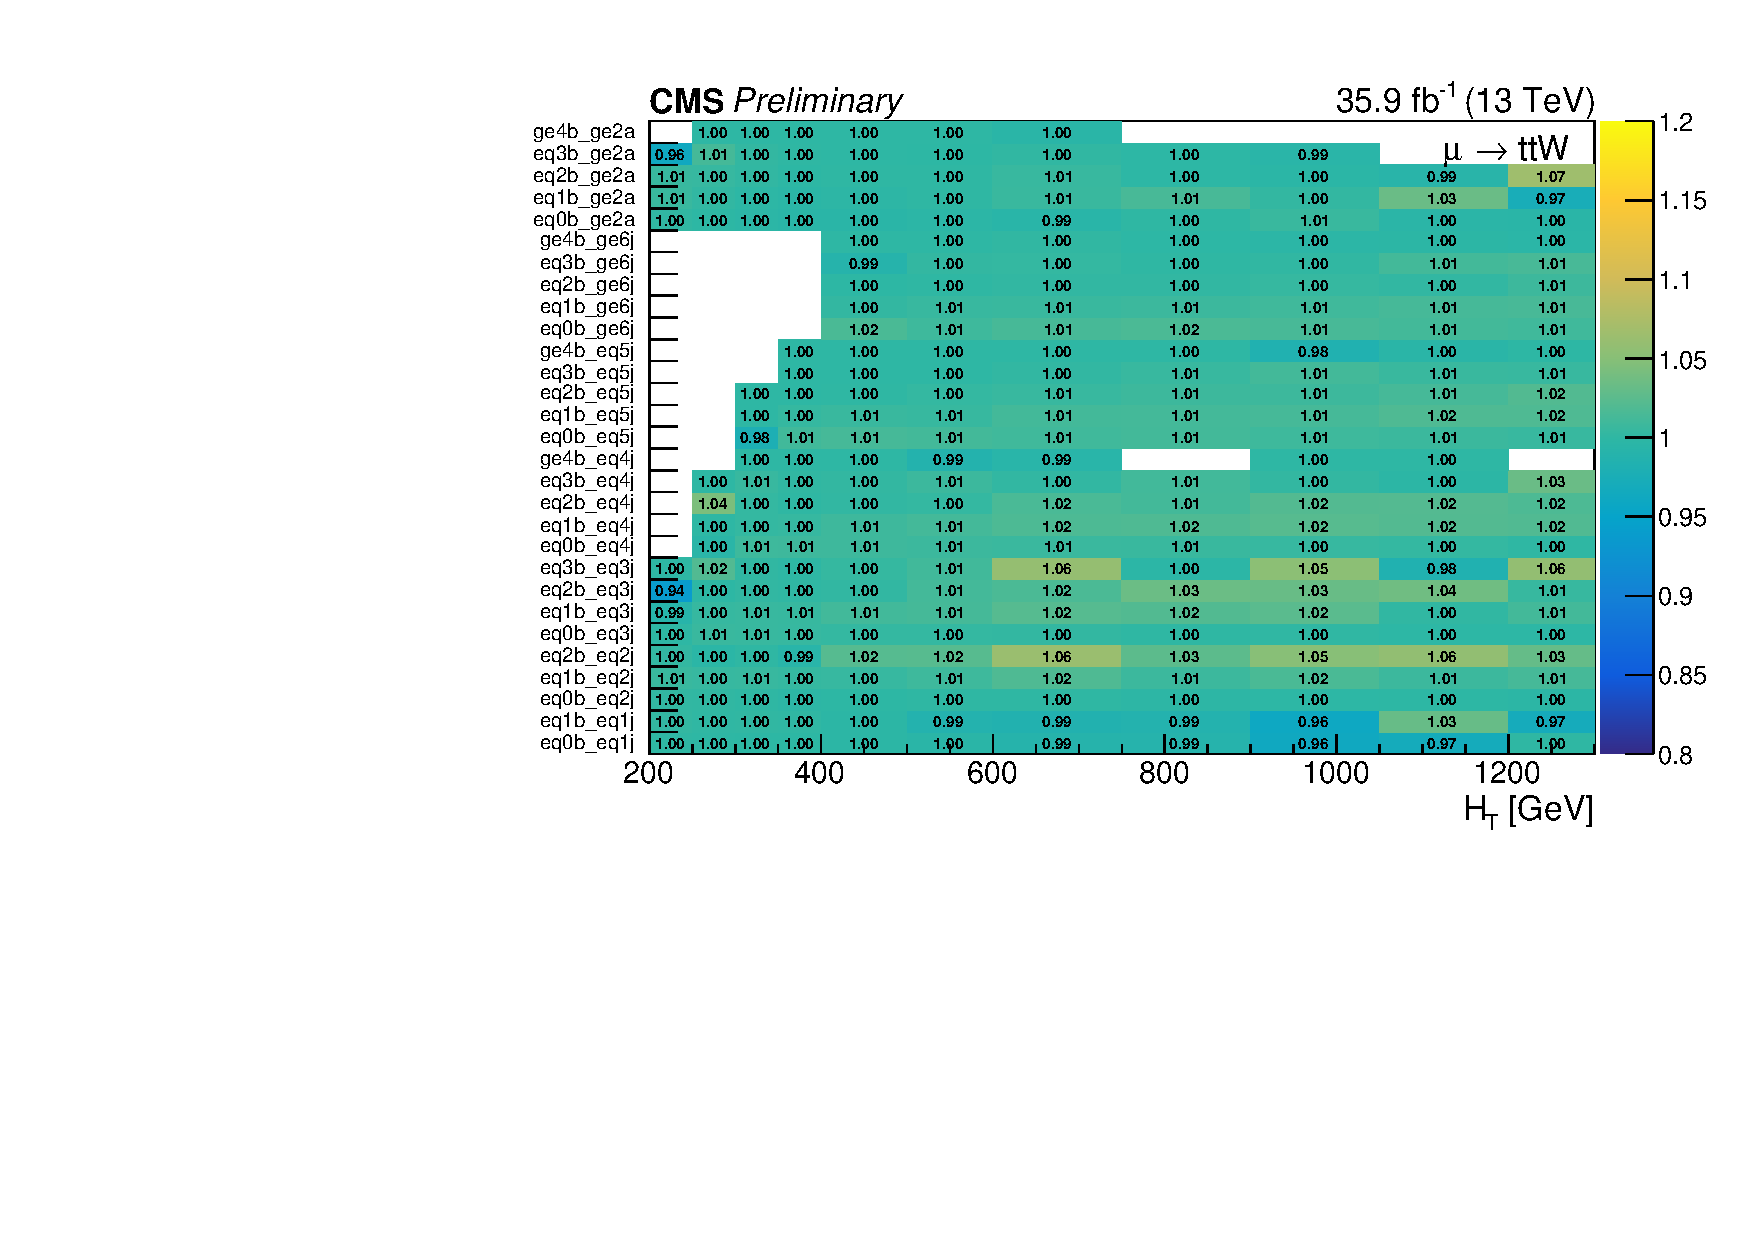
\includegraphics[width=0.5\textwidth]{figs/analysis/transferfactors/tfratio_mu_Ttw_2d_xsWeightWUp}}~
	\subfloat{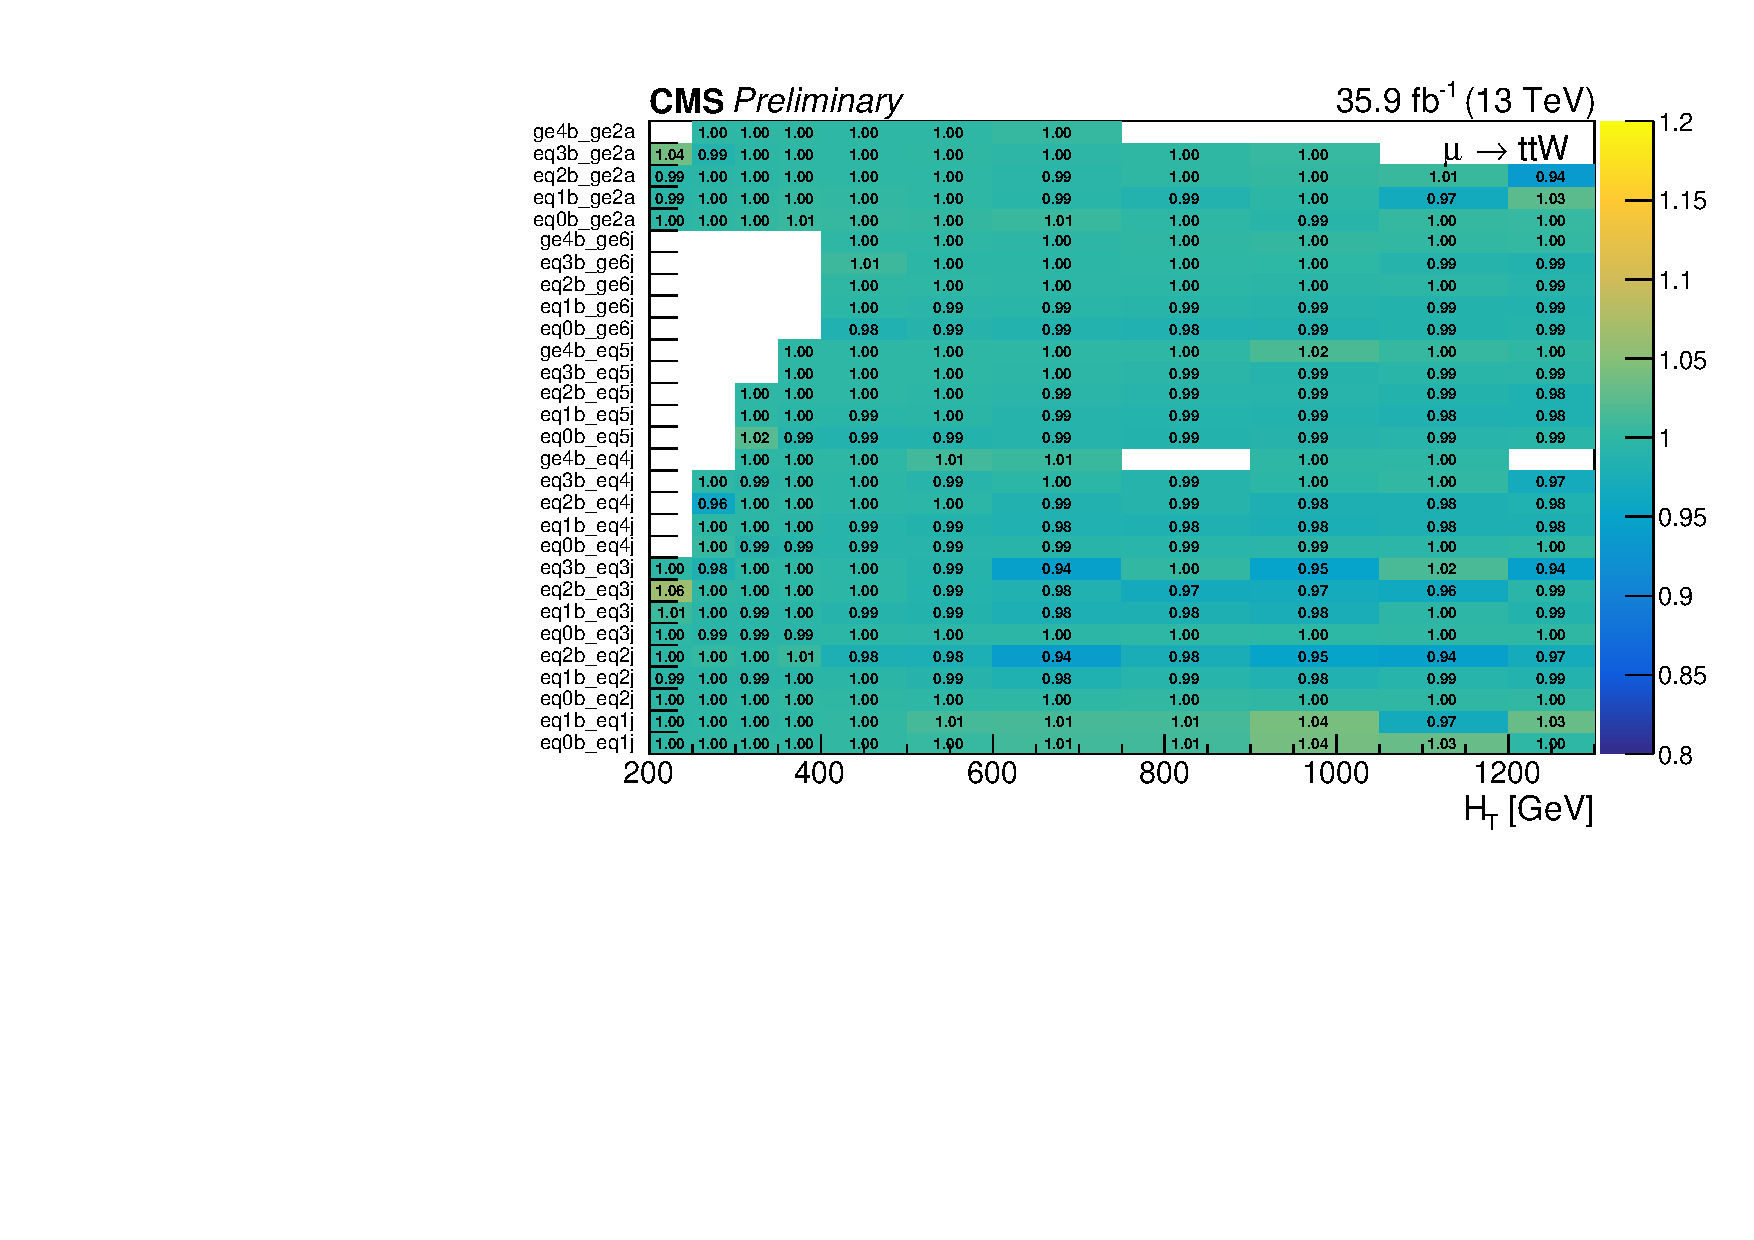
\includegraphics[width=0.5\textwidth]{figs/analysis/transferfactors/tfratio_mu_Ttw_2d_xsWeightWDown}}\\
	\subfloat{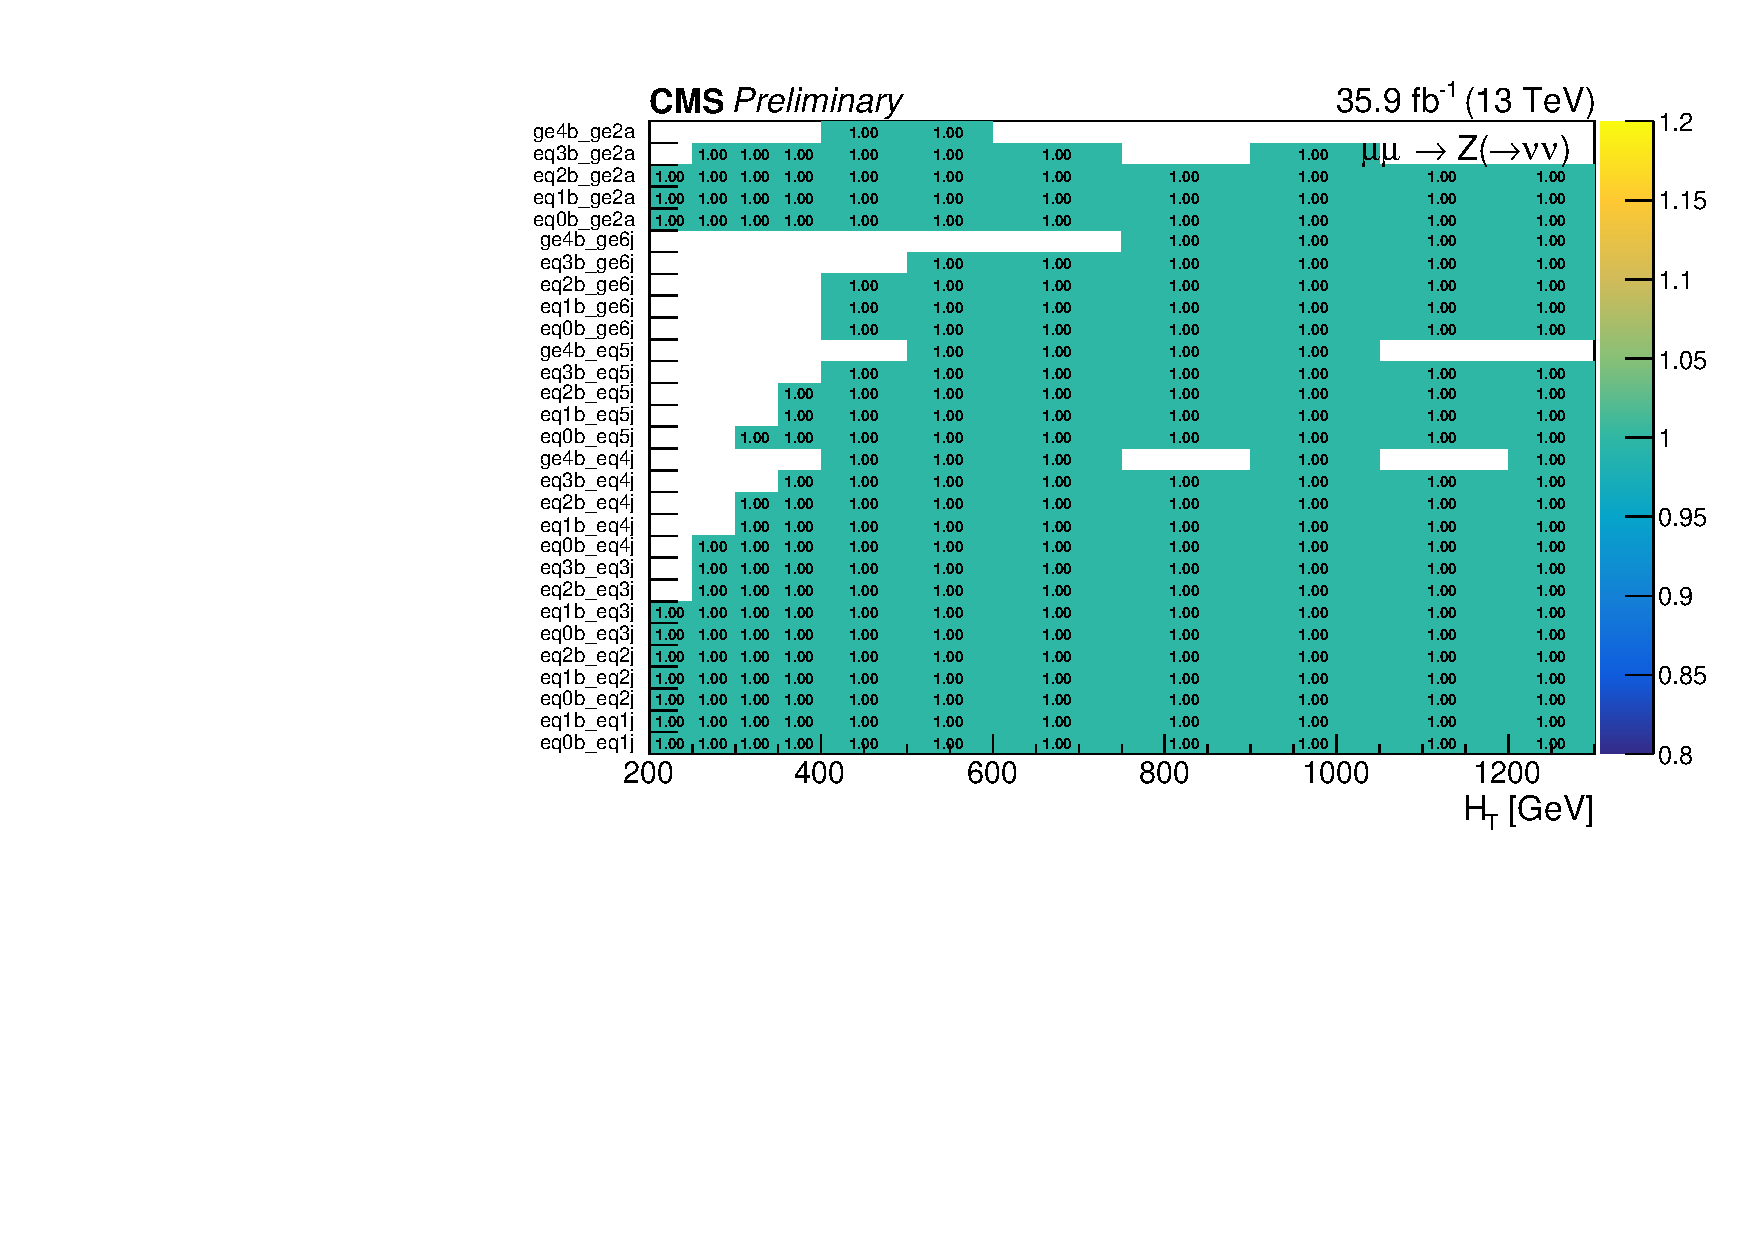
\includegraphics[width=0.5\textwidth]{figs/analysis/transferfactors/tfratio_mumu_Zinv_2d_xsWeightWUp}}~
	\subfloat{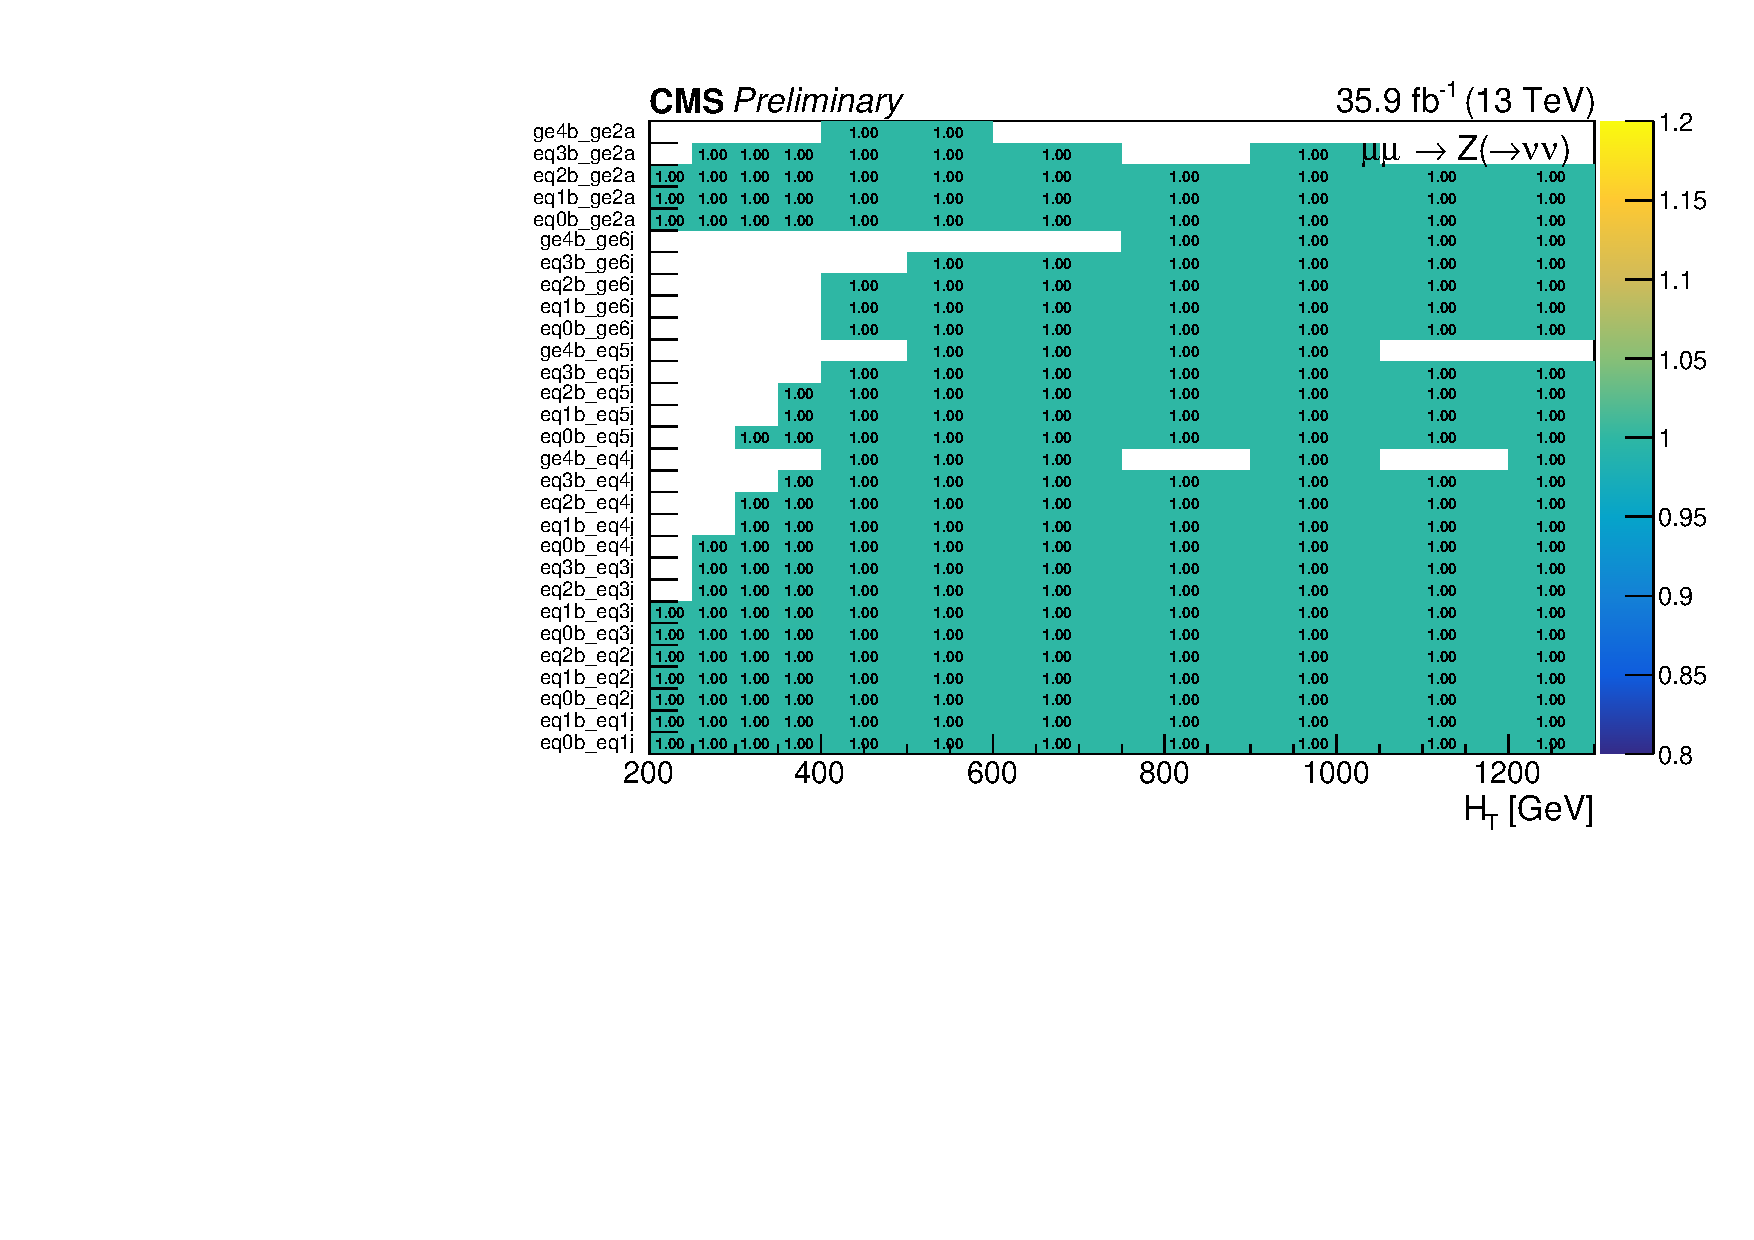
\includegraphics[width=0.5\textwidth]{figs/analysis/transferfactors/tfratio_mumu_Zinv_2d_xsWeightWDown}}\\
	\caption{The ratio of the \Tmutottw (top) and \Tmumutoz (bottom) transfer 
		factors in each \njnbht bin when varying the W cross section correction 
		factors by $+1\sigma$ (left) and $-1\sigma$ (right) with respect to 
		their nominal values.}
	\label{fig:tfvariations-xsw}
\end{figure}

\begin{figure}[h!]
	\subfloat{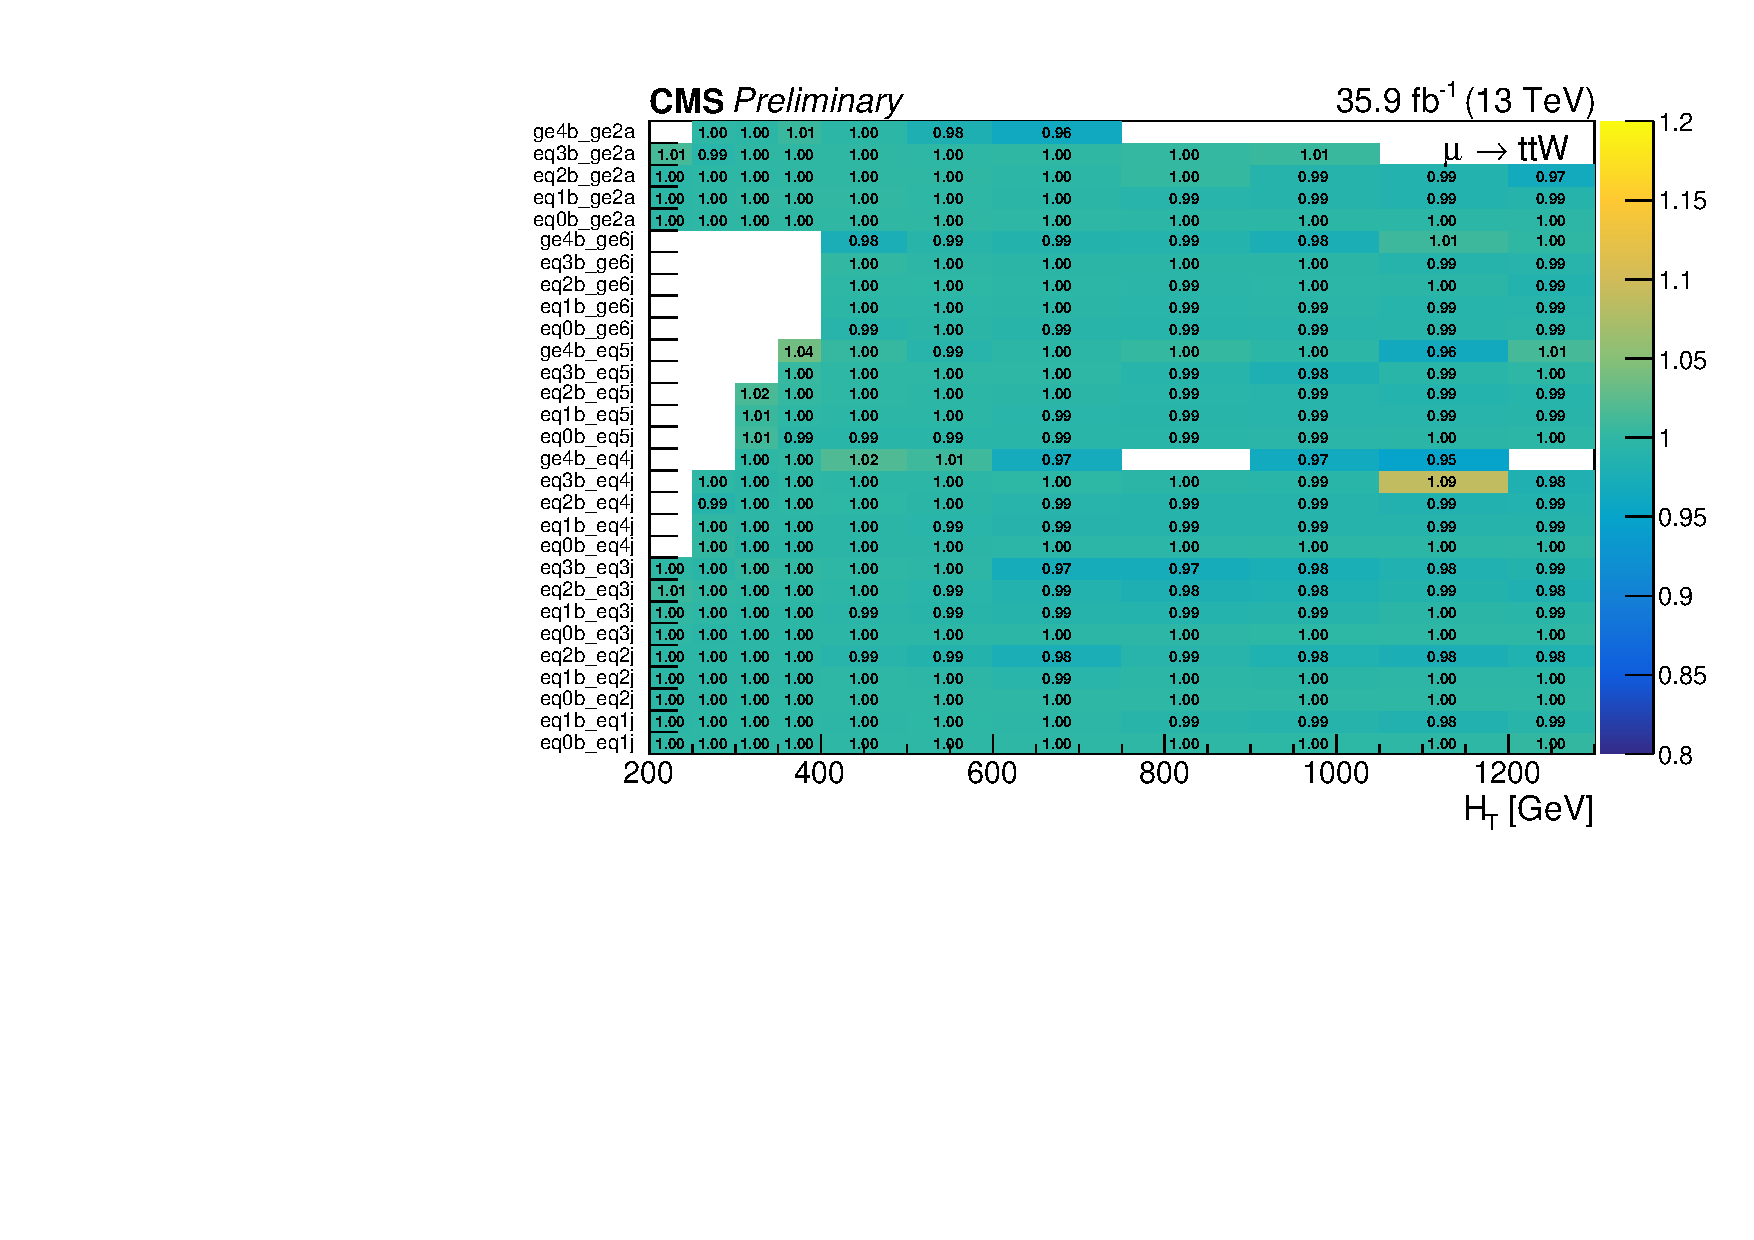
\includegraphics[width=0.5\textwidth]{figs/analysis/transferfactors/tfratio_mu_Ttw_2d_xsWeightTtUp}}~
	\subfloat{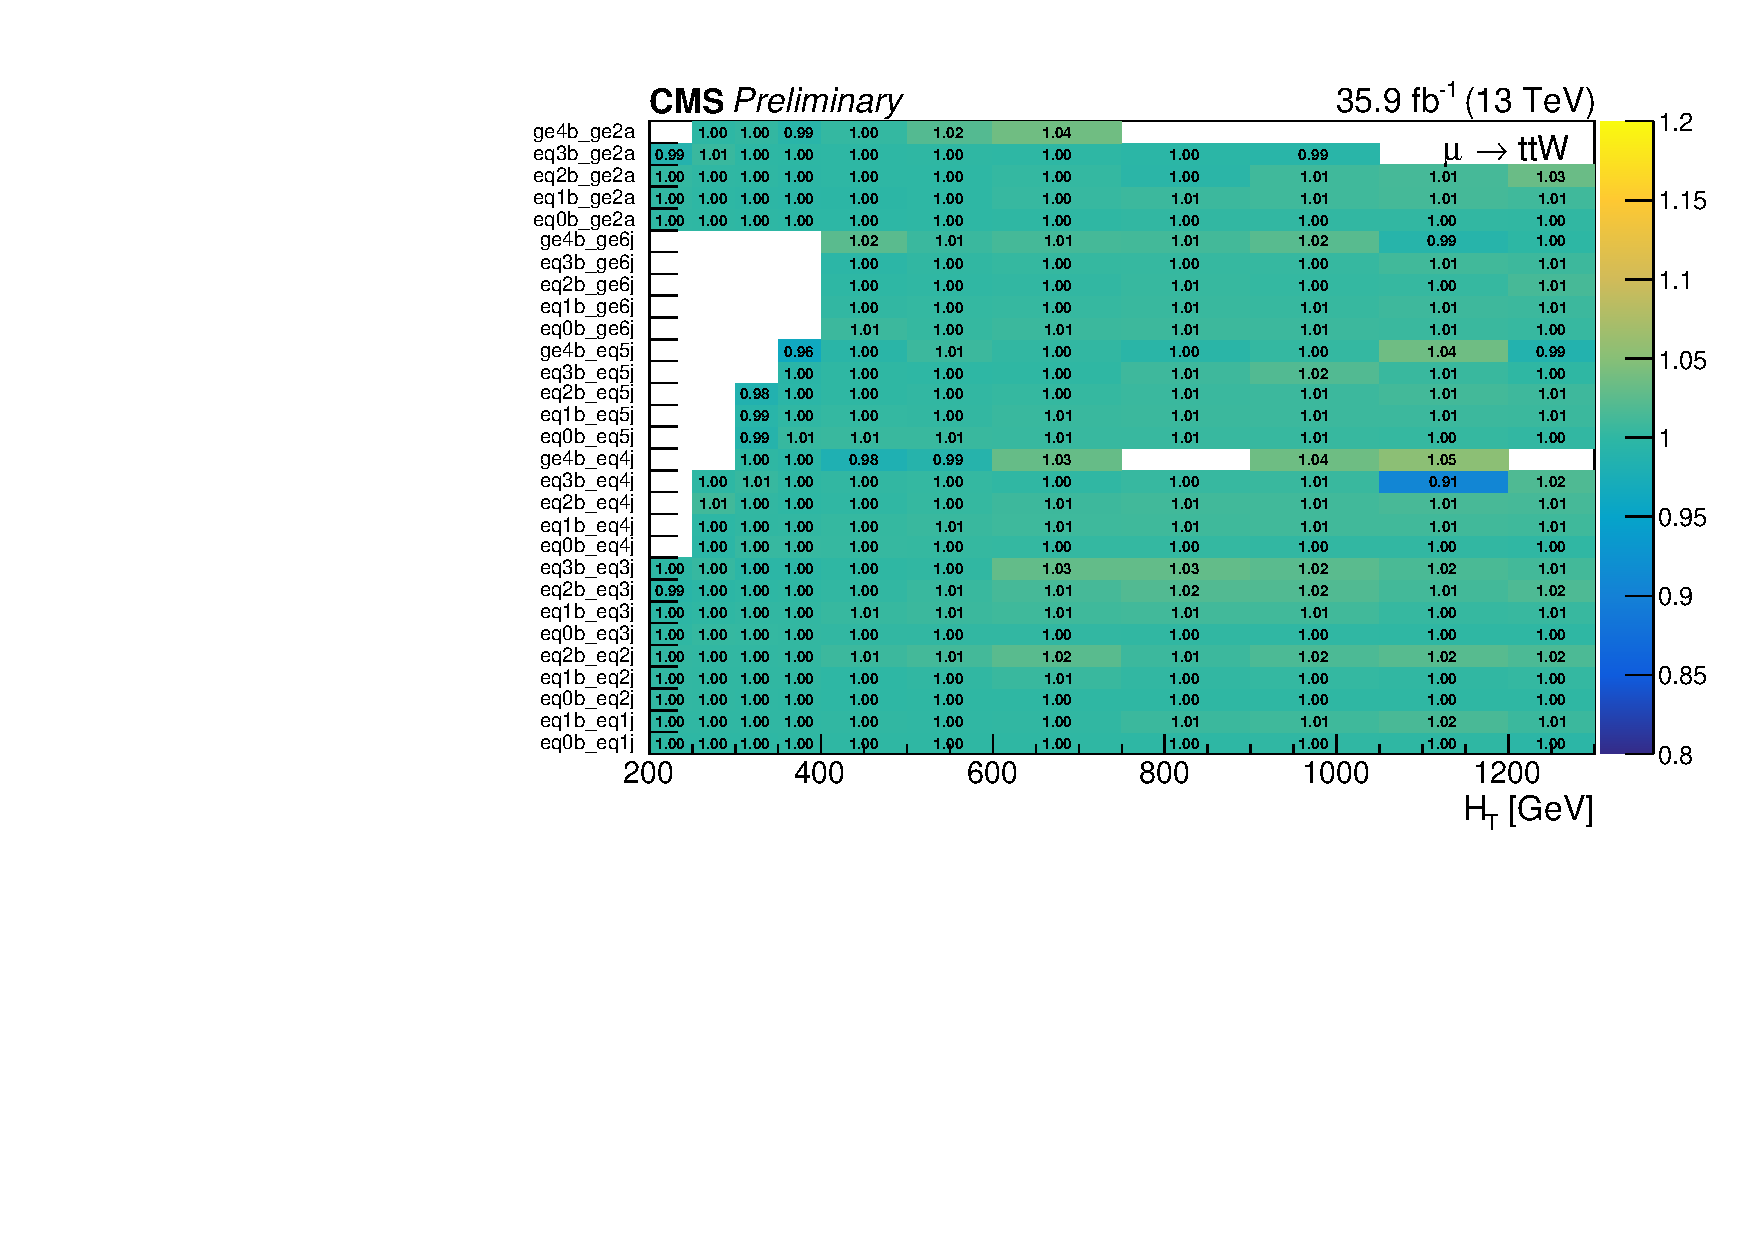
\includegraphics[width=0.5\textwidth]{figs/analysis/transferfactors/tfratio_mu_Ttw_2d_xsWeightTtDown}}\\
	\subfloat{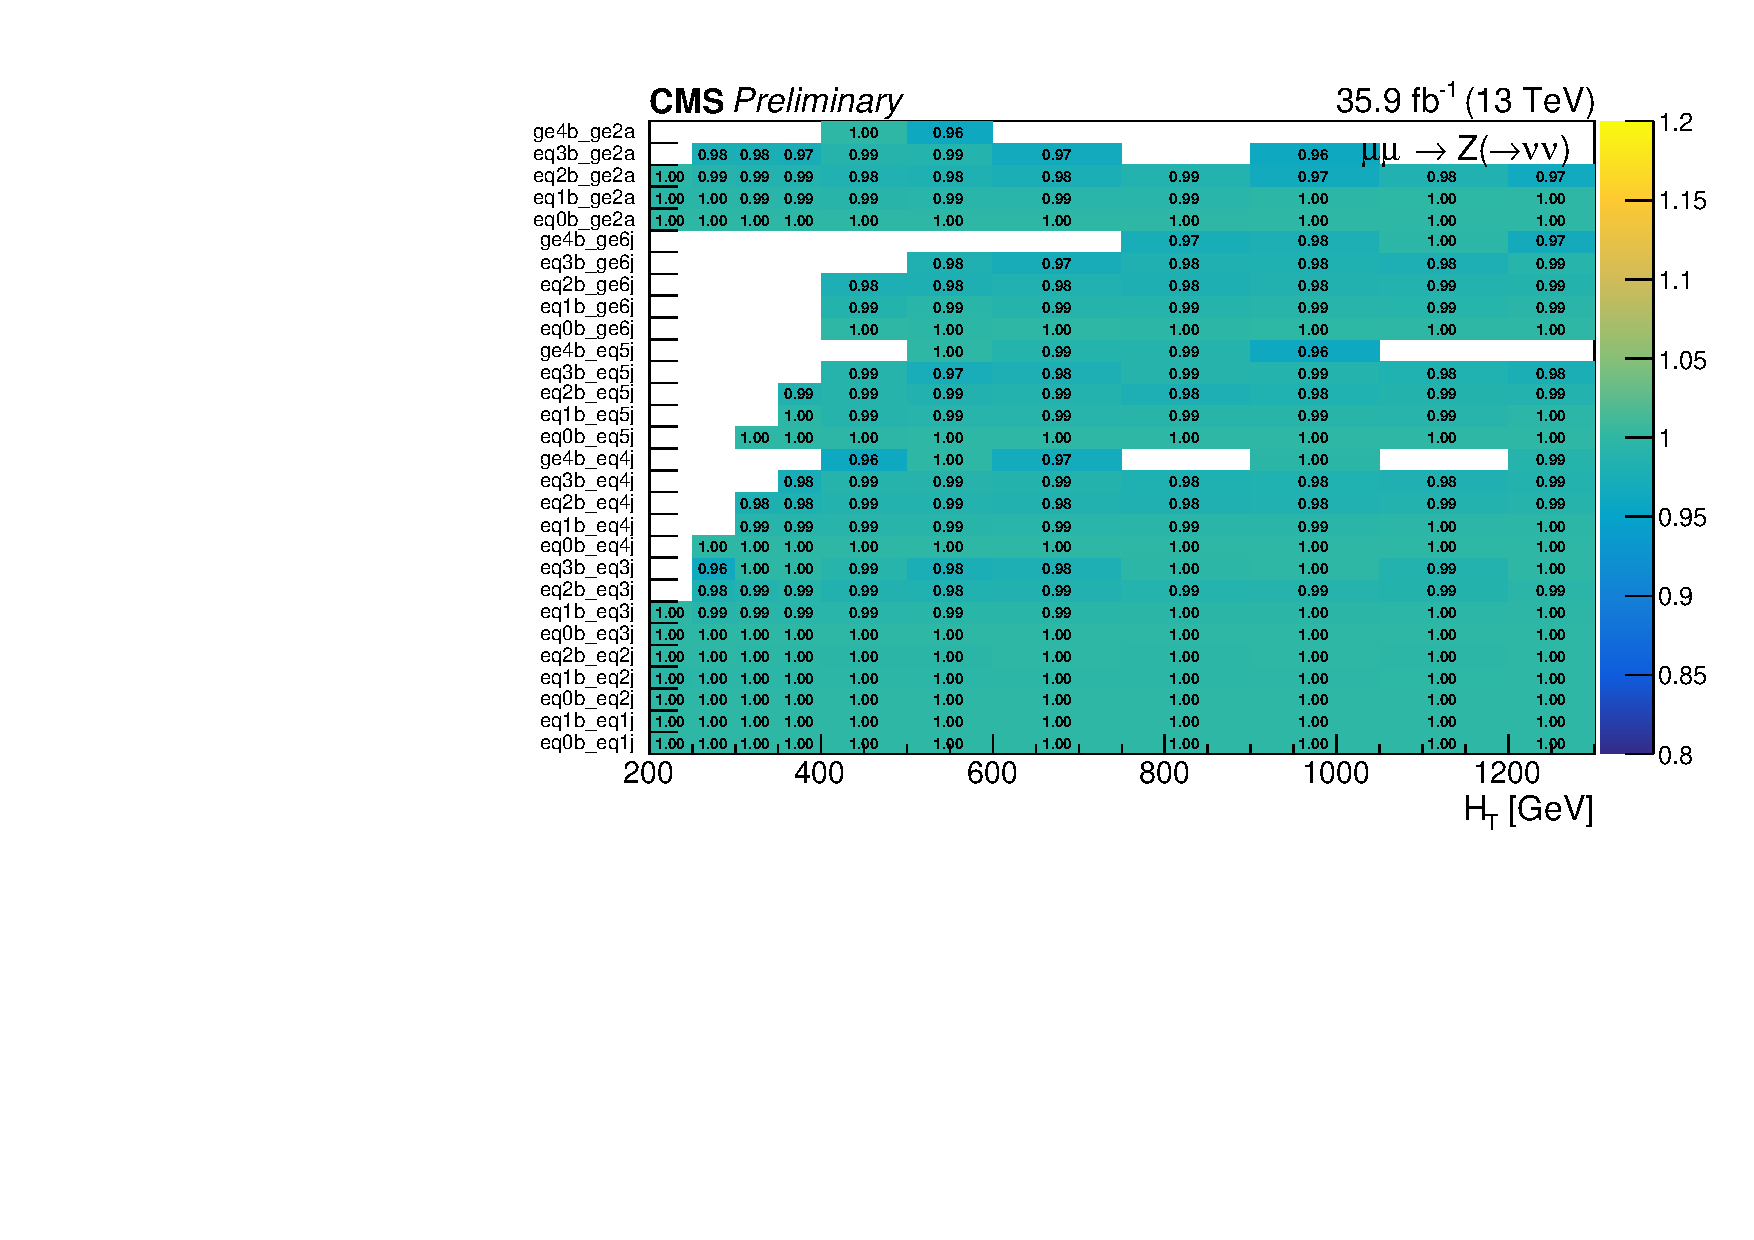
\includegraphics[width=0.5\textwidth]{figs/analysis/transferfactors/tfratio_mumu_Zinv_2d_xsWeightTtUp}}~
	\subfloat{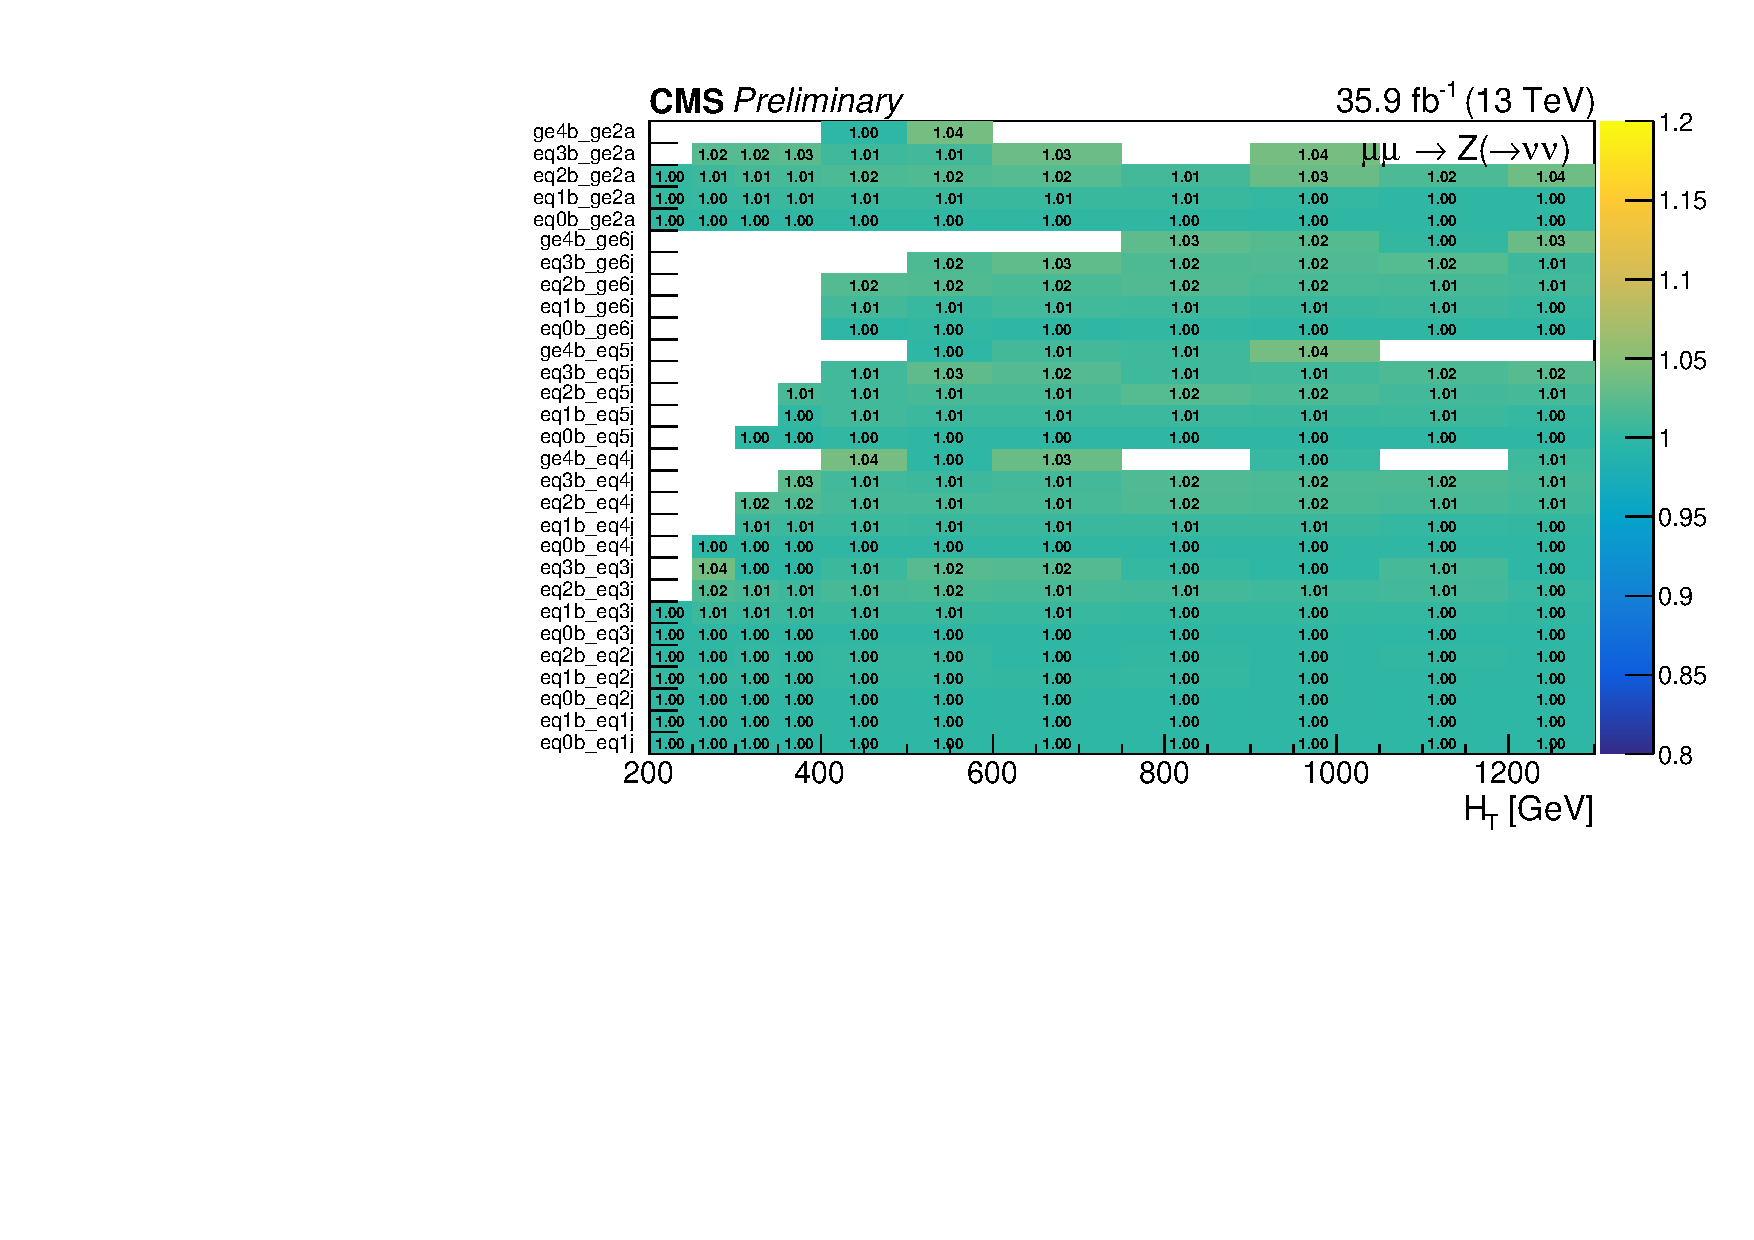
\includegraphics[width=0.5\textwidth]{figs/analysis/transferfactors/tfratio_mumu_Zinv_2d_xsWeightTtDown}}\\
	\caption{The ratio of the \Tmutottw (top) and \Tmumutoz (bottom) transfer 
		factors in each \njnbht bin when varying the \ttbar cross section 
		correction factors by $+1\sigma$ (left) and $-1\sigma$ (right) with 
		respect to 
		their nominal values.}
	\label{fig:tfvariations-xsttw}
\end{figure}



%\chapter{Systematics}
%\label{app:systs}
%Hi.